\documentclass{report}
\usepackage[utf8]{inputenc}
\usepackage[romanian]{babel}
\usepackage{graphicx}
\usepackage{hyperref}
\usepackage{amsmath}
\usepackage{amsfonts}
\usepackage{amssymb}
\usepackage{listings}
\usepackage{float}
\usepackage{caption}
\usepackage{fancyhdr}
\usepackage{fontspec}
\usepackage{polyglossia}
\usepackage{url}
\usepackage{color}
\usepackage{xcolor}
\usepackage{setspace}
\usepackage{titlesec}
\usepackage{media9}
\usepackage{hyperref}
\usepackage{listings}
\lstset{
    basicstyle=\ttfamily,
    frame=single,
    breaklines=true
}

\definecolor{codebg}{rgb}{0.95,0.95,0.95}
\definecolor{codeframe}{rgb}{0.75,0.75,0.75}
\definecolor{myblue}{rgb}{0.0, 0.0, 1.0} % Defineste o nuanta de albastru

\setmainlanguage{romanian}

\setmainfont{UTSans-Regular.ttf}[
    BoldFont = UTSans-Bold.ttf,
    ItalicFont = UTSans-Regular.ttf,
    BoldItalicFont = UTSans-Bold.ttf
]
\newfontfamily\headingfont{UTSans-Medium.ttf}

% Configurarea antetului
\fancypagestyle{plain}{
    \fancyhf{} % Curatam anteturile si subsolurile existente
    \fancyhead[L]{\hspace*{-5cm}\vspace*{-1cm}
\includegraphics[width=7cm]{logo.jpg}} 
    
    \renewcommand{\headrulewidth}{0pt} % Linie sub antet
    \fancyfoot[R]{\begin{picture}(0,0)\put(-42,-13){\textbf{\large □}}\end{picture}\thepage} % Pătrat în colțul din dreapta sus
}

\pagestyle{plain} %Se aplica stilul pentru toate paginile
\pagenumbering{gobble}

% Setează culoarea titlurilor
\titleformat{\chapter}[display]
  {\normalfont\Huge\bfseries\color{myblue}} % Titluri de capitol
  {\chaptername\ \thechapter}{20pt}{\Huge}
  
\titleformat{\section}
  {\normalfont\Large\bfseries\color{myblue}} % Titluri de sectiune
  {\thesection}{1em}{}
  
\titleformat{\subsection}
  {\normalfont\large\bfseries\color{myblue}} % Titluri de subsectiune
  {\thesubsection}{1em}{}

\begin{document}

\begin{center}
\vspace*{3cm}
{\headingfont\huge Sistem de acces cu recunoaștere facială folosind Arduino\par}
{\headingfont\small Coordonator : Dinu Alexandru \par}
\vspace{3cm}
{\Large LUCRARE DE LABORATOR\par}
\vspace{2cm}
{\small BRAȘOV, 2024\par}
\vfill
\end{center}

\pagenumbering{arabic}
\vspace*{3cm}

\tableofcontents
\thispagestyle{empty} % Elimină antetul doar pe această pagină


\chapter{Obiectivele lucrării}
Scopul acestui proiect este de a implementa un sistem de acces controlat prin recunoașterea facială, utilizând o placă Arduino Uno și perifericele sale. Proiectul își propune să demonstreze utilizarea registrelor și a programării la nivel hardware pentru controlul unor periferice cum ar fi un motor servo și să ofere o soluție practică pentru securitatea fizică. 
De asemenea, se urmărește învățarea și aplicarea conceptelor de recunoaștere facială și control automatizat al accesului, precum și utilizarea componentelor de feedback vizual, cum ar fi LCD-ul și LED-urile, cât și reglarea intensițății acestora cu ajutorul unui potențiometru.
În acelși timp oferă oportunitatea de a lucra cu limbajul de programare python, deoarece proiectul conține un mic script folosit ca suport pentru recunoașterea facială, care preia imaginile captate de ESP, de la url-ul generat prin Espressif, iar apoi în funcție de verificare transmite mesajele corespunzătoare dispozitivelor de ieșire. 
Astfel proiectul oferă studeților mai multe posibilițăți de dezvoltare și aprofundare. Pe de o parte este cea hardware, în care studeții vor învața modul în care interacționeaza componentele între ele și legăturile dintre acestea, datorită Arduino, iar pe de altă parte intrervine partea de software prin programarea în limbajul python. De asemenea apare și programarea la nivel de regiștrii, proiectul reprezentând astfel o posiblitate prin care studenții să își dea seama despre ramura care îi atrage mai mult, experimentand aici câte puțin din toate.   
\chapter{Aspecte teoretice}

\section{Arduino - Introducere și Caracteristici}
Arduino este o platformă open-source folosită pentru prototiparea electronică. Aceasta combină hardware-ul (placa Arduino) și software-ul (Arduino IDE) pentru a permite dezvoltatorilor să creeze proiecte interactive. Principalele caracteristici includ:

\begin{itemize}
    \item \textbf{Microcontroler:} Plăcile Arduino sunt echipate cu microcontrolere precum ATmega328, care gestionează toate operațiunile.
    \item \textbf{Pini I/O:} Plăcile au pini digitali și analogici pentru interacțiunea cu senzori și actuatori.
    \item \textbf{Alimentare:} Pot fi alimentate prin USB sau printr-o sursă externă (5V-12V).
    \item \textbf{Programare:} Codul este scris într-un limbaj similar cu C/C++ și încărcat pe placă prin intermediul unui bootloader.
    \item \textbf{Biblioteci:} Arduino oferă numeroase biblioteci pentru simplificarea interacțiunii cu senzori, motoare sau alte componente.
\end{itemize}

\section{Python - Limbaj de Programare}
Python este un limbaj de programare de nivel înalt, cunoscut pentru ușurința în utilizare și comunitatea sa activă. Este frecvent utilizat pentru procesarea datelor, inteligență artificială și control hardware. 

\begin{itemize}
    \item \textbf{Ușor de învățat:} Sintaxa simplă permite utilizatorilor să dezvolte rapid aplicații complexe.
    \item \textbf{Portabilitate:} Este multi-platformă, funcționând pe Windows, MacOS și Linux.
    \newpage
    \vspace*{1cm}
    \item \textbf{Biblioteci puternice:} Există librării precum `OpenCV` pentru procesarea imaginilor și `Serial` pentru comunicarea cu hardware.
\end{itemize}

\section{Programarea pe Regiștri}
Programarea pe regiștrii implică controlul direct al hardware-ului prin scrierea și citirea regiștrilor microcontrolerului. Aceasta este o metodă avansată, dar esențială pentru înțelegerea detaliată a funcționării interne a plăcilor Arduino, pe baza informațiilor din datasheets.

\begin{itemize}
    \item \textbf{Registre de Configurare:} Determină funcția unui pin (input/output) și setările acestuia.
    \item \textbf{Întreruperi:} Se utilizează pentru a răspunde la evenimente externe sau interne, fără a bloca execuția programului principal.
    \item \textbf{Timeri și Contoare:} Gestionarea temporizării exacte și a frecvențelor PWM pentru controlul motoarelor.
    \item \textbf{UART:} Comunicare serială între dispozitive (ESP32 și Arduino în cazul nostru).
\end{itemize}

\section{Integrarea Arduino-Python}
Integrarea dintre Arduino și Python permite utilizatorilor să combine avantajele ambelor platforme. În acest proiect:
\begin{itemize}
    \item Arduino controlează perifericele hardware.
    \item Python rulează pe un PC pentru procesarea imaginilor și comunică cu Arduino prin protocolul serial.
\end{itemize}

\textbf{Obiective principale}:
\begin{enumerate}
    \item Implementarea unui sistem de recunoaștere facială pentru autorizarea accesului, care poate învăța și valida fețele utilizatorilor.
    \item Utilizarea registrelor interne pentru controlul motorului servo prin PWM (Pulse Width Modulation), asigurând o acționare precisă a mecanismului de deschidere.
    \item Integrarea camerei ESP32-CAM pentru capturarea și procesarea imaginilor, utilizând resursele disponibile ale microcontrolerului.
    \newpage
    \vspace*{1cm}
    \item Testarea și validarea funcționalității sistemului, asigurându-se că acesta funcționează corect și îndeplinește cerințele specificate.
\end{enumerate}

Din această lucrare, studenții vor învăța:
\begin{itemize}
    \item Cum să interacționeze cu perifericile direct prin programarea registrelor ATmega328.
    \item Cum să configureze un sistem bazat pe recunoaștere facială utilizând un modul extern, gestionând fluxul de date între diferite componente.
    \item Cum să controleze un motor servo folosind semnale PWM generate de Arduino, aplicând conceptele de bază ale controlului motorului în proiecte reale.
\end{itemize}

\begin{figure}[H]
    \centering
    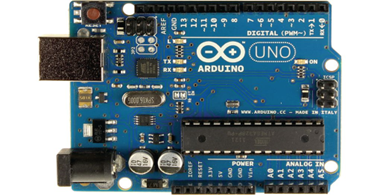
\includegraphics[width=0.6\textwidth]{arduino.png}
    \caption{Placa Arduino Uno}
    \label{fig:arduino}
\end{figure}

\begin{figure}[H]
    \centering
    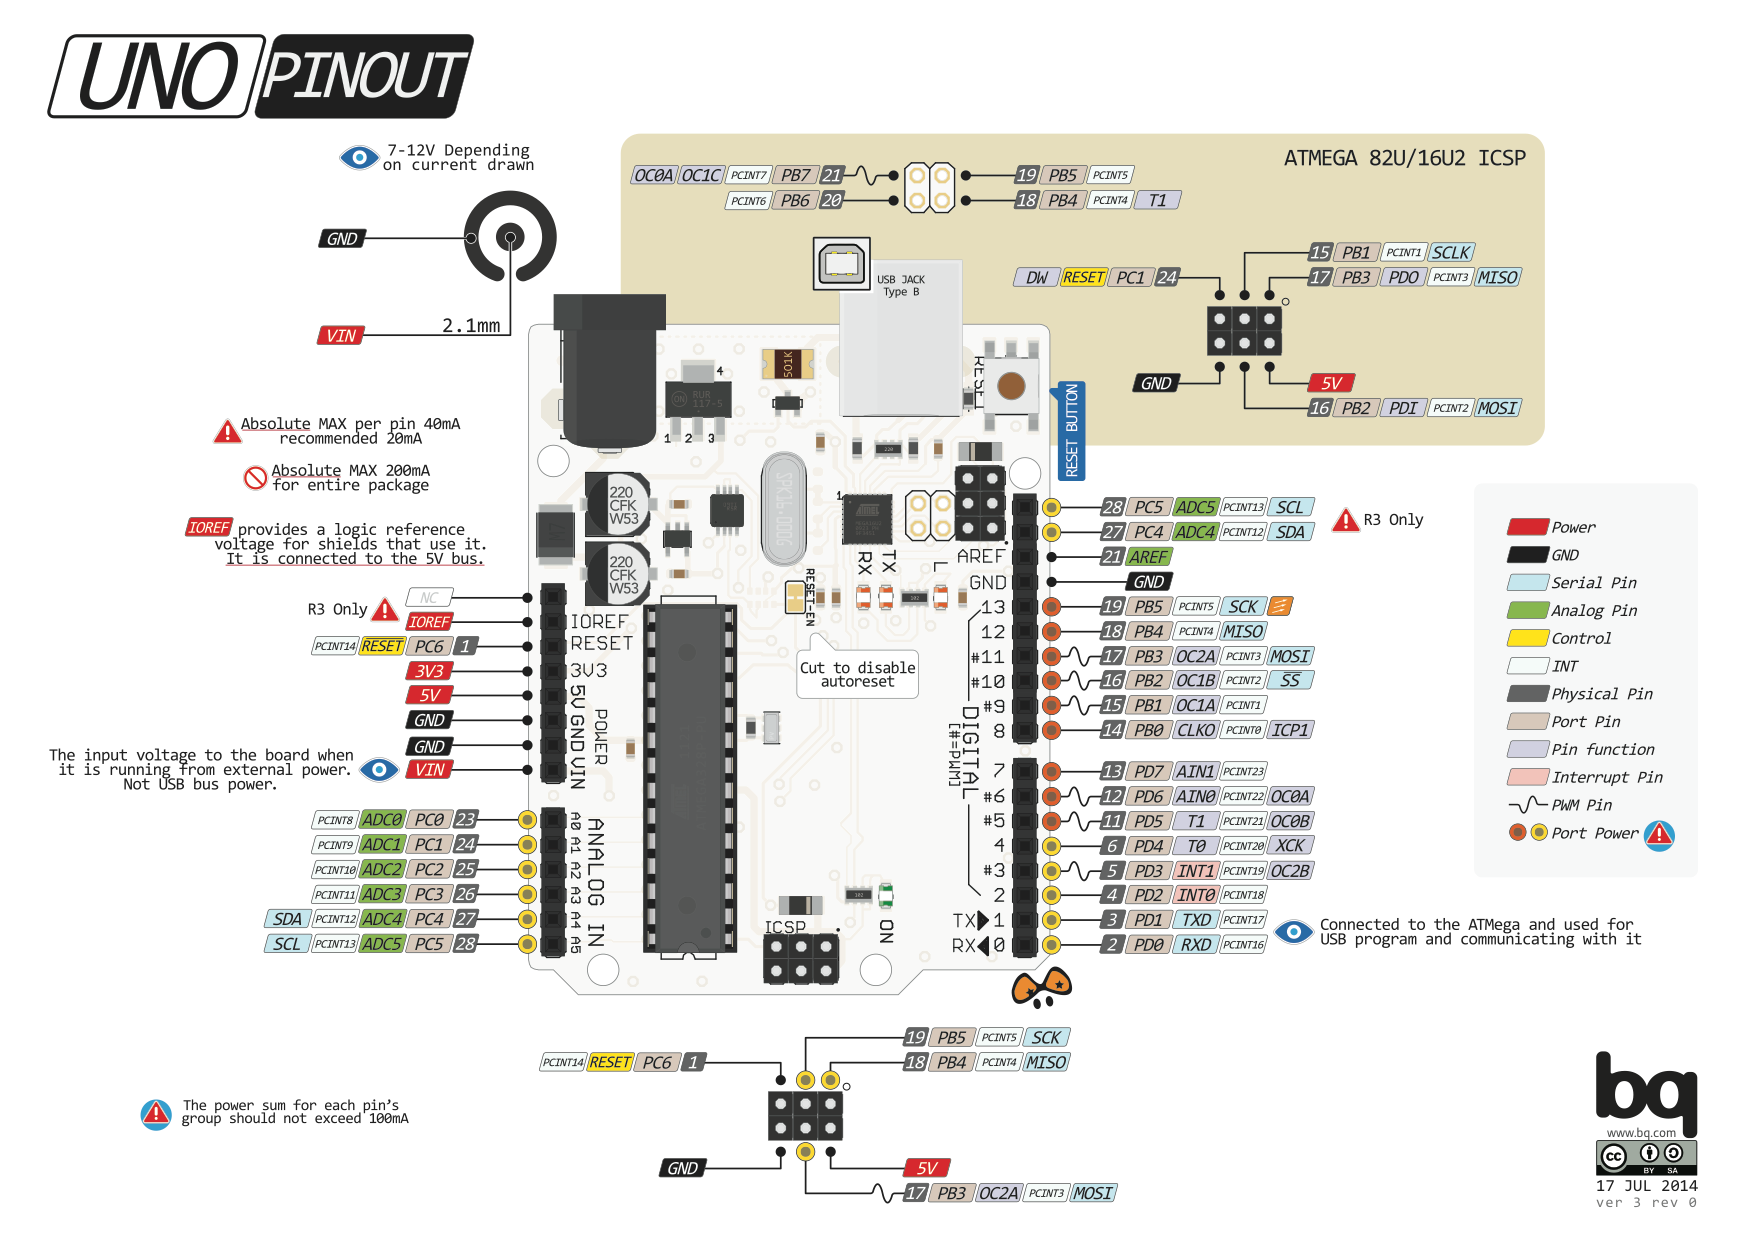
\includegraphics[width=0.6\textwidth]{Arduino-uno-pinout.png}
    \caption{Schema pinilor plăcii Arduino Uno}
    \label{fig:arduino_pinout}
\end{figure}


\newapge
\vspace*{1cm}
Porturile de pe placa Arduino Uno sunt împărțite în trei grupe principale:

\begin{itemize}
    \item \textbf{Portul B:} corespunde pinilor digitali de la 8 la 13.
    \item \textbf{Portul C:} corespunde pinilor analogici de intrare.
    \item \textbf{Portul D:} corespunde pinilor digitali de la 0 la 7.
\end{itemize}

Fiecare port este controlat prin intermediul a trei registre:
\begin{itemize}
    \item \textbf{Registrul DDR (Data Direction Register):} determină direcția pinului (intrare sau ieșire). Acesta este echivalentul funcției \texttt{pinMode()} din limbajul Arduino.
    \item \textbf{Registrul PORT:} controlează starea pinului (HIGH sau LOW) pentru ieșiri și activează rezistențele de pull-up pentru intrări.
    \item \textbf{Registrul PIN:} permite citirea stării unui pin setat ca intrare.
\end{itemize}

Caracteristicile registrelor:
\begin{itemize}
    \item Atât \textbf{DDR} cât și \textbf{PORT} pot fi scrise și citite.
    \item Registrul \textbf{PIN} este read-only și oferă starea curentă a pinului (HIGH sau LOW).
    \item Fiecare bit din aceste registre corespunde unui pin specific din portul respectiv.
\end{itemize}

Cele trei porturi utilizate în placa Arduino Uno sunt:
\begin{itemize}
    \item \textbf{PORTD (DDRD, PORTD, PIND):} gestionează pinii digitali de la 0 la 7.
    \item \textbf{PORTB (DDRB, PORTB, PINB):} gestionează pinii digitali de la 8 la 13.
    \item \textbf{PORTC (DDRC, PORTC, PINC):} gestionează pinii analogici de intrare.
\end{itemize}

\begin{figure}[H]
    \centering
    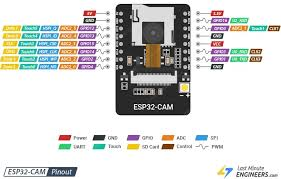
\includegraphics[width=0.7\textwidth]{imageEsp.jpeg}
    \caption{Schema pinilor plăcii ESP32-CAM}
    \label{fig:esp32_cam_pinout}
\end{figure}

\newpage
\vspace*{1cm}
Placa ESP32-CAM este un modul compact cu o cameră integrată, utilizat frecvent pentru proiecte IoT și de recunoaștere a imaginilor. Conectorii săi principali includ:

\begin{itemize}
    \item \textbf{GPIO (General Purpose Input/Output):} pini digitali configurabili pentru intrare sau ieșire.
    \item \textbf{UART (Universal Asynchronous Receiver-Transmitter):} pini dedicați pentru comunicații seriale.
    \item \textbf{SPI (Serial Peripheral Interface):} pini pentru comunicații rapide cu periferice, cum ar fi carduri SD.
    \item \textbf{Touch:} pini sensibili la atingere, care pot detecta variații capacitive.
    \item \textbf{Power (5V/3.3V):} pini pentru alimentare, atât pentru modulele interne cât și pentru perifericele externe.
    \item \textbf{GND (Ground):} pini pentru referința la masă.
    \item \textbf{SD Card Interface:} pini pentru comunicarea cu un card SD, precum \texttt{HSPI\_CLK}, \texttt{HSPI\_CMD}, și \texttt{HSPI\_Q}.
    \item \textbf{PWM (Pulse Width Modulation):} pini folosiți pentru generarea semnalelor PWM pentru controlul dispozitivelor precum LED-uri sau servomotoare.
\end{itemize}

Acest pinout este esențial pentru interfațarea ESP32-CAM cu senzori, module de memorie (SD card) și alte dispozitive externe, oferind flexibilitate în utilizare pentru proiecte avansate.




\chapter{Descrierea componentelor}

\section{Componente hardware:}
\begin{itemize}
    \item \textbf{Arduino Uno}: Microcontrolerul principal utilizat pentru gestionarea perifericelor și controlul logicii.
    \begin{itemize}
        \item Microcontroler: ATmega328P.
        \item Pini I/O digitali: 14 (dintre care 6 suportă PWM).
        \item Pini analogici: 6.
        \item Tensiune de operare: 5V.
        \item Memorie Flash: 32 KB.
        \item Frecvență de lucru: 16 MHz.
    \end{itemize}
    \begin{figure}[H]
    \centering
    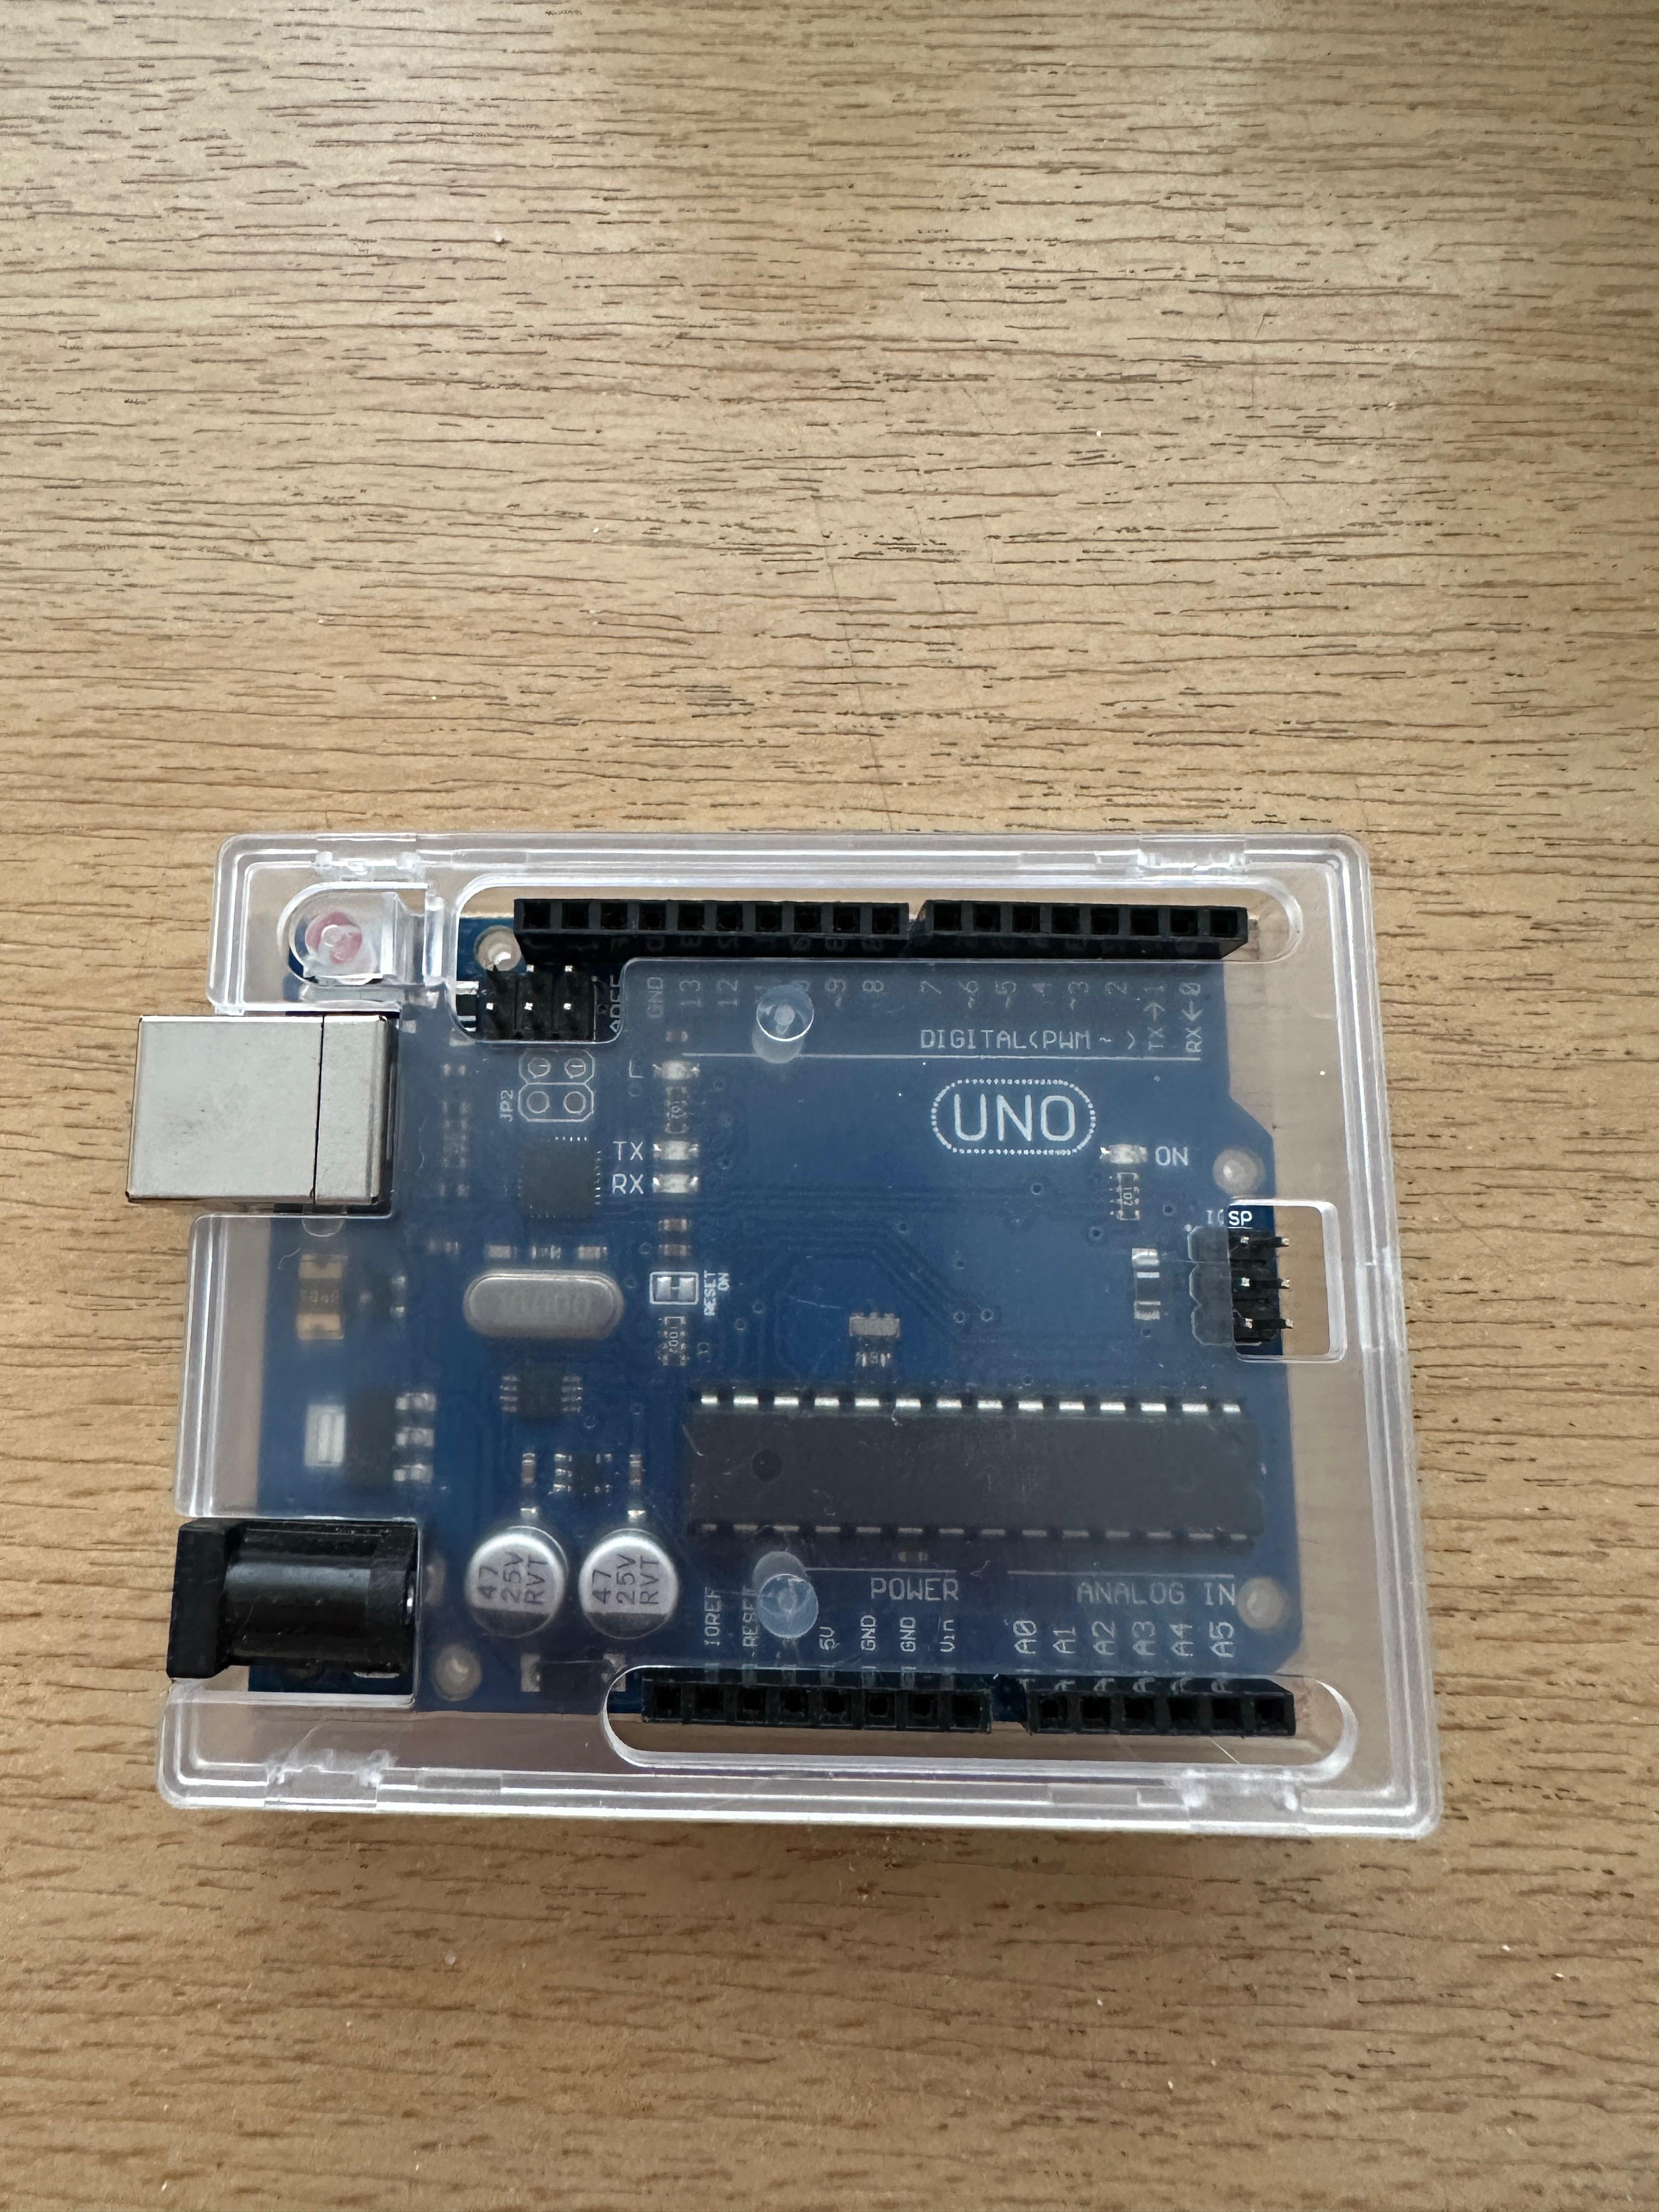
\includegraphics[width=0.4\textwidth]{arduino.jpg}
    \caption{Arduino Uno}
    \label{fig:earduino}
\end{figure}
    
\vspace*{1cm}
    \item \textbf{ESP32-CAM}: Modul pentru capturarea imaginii feței, care va transmite datele către Arduino pentru verificare. Imaginile capturate de ESP32-CAM sunt comparate cu fișiere autorizate utilizând un script Python, iar rezultatele sunt transmise către dispozitivele de ieșire.
    \begin{itemize}
        \item Procesor: Dual-core Xtensa LX6 (240 MHz).
        \item Memorie: 520 KB SRAM + 4 MB PSRAM.
        \item Interfață: UART, SPI, I2C.
        \item Cameră: OV2640 cu suport pentru imagini de până la 1600x1200.
        \item Alimentare: VCC conectat la 5V.
        \item Pini:
            \begin{itemize}
                \item VCC: conectat la 5V pe Arduino.
                \item GND: conectat la GND pe Arduino.
                \item TX (Transmit): conectat la TX de pe Arduino.
                \item RX (Receive): conectat la un RX de pe Arduino.
                
                \vspace*{1cm}
                \item GPIO: pentru intrare în modul de programare, se conectează GPIO la GND.
            \end{itemize}
    \end{itemize}
    \begin{figure}[H]
    \centering
    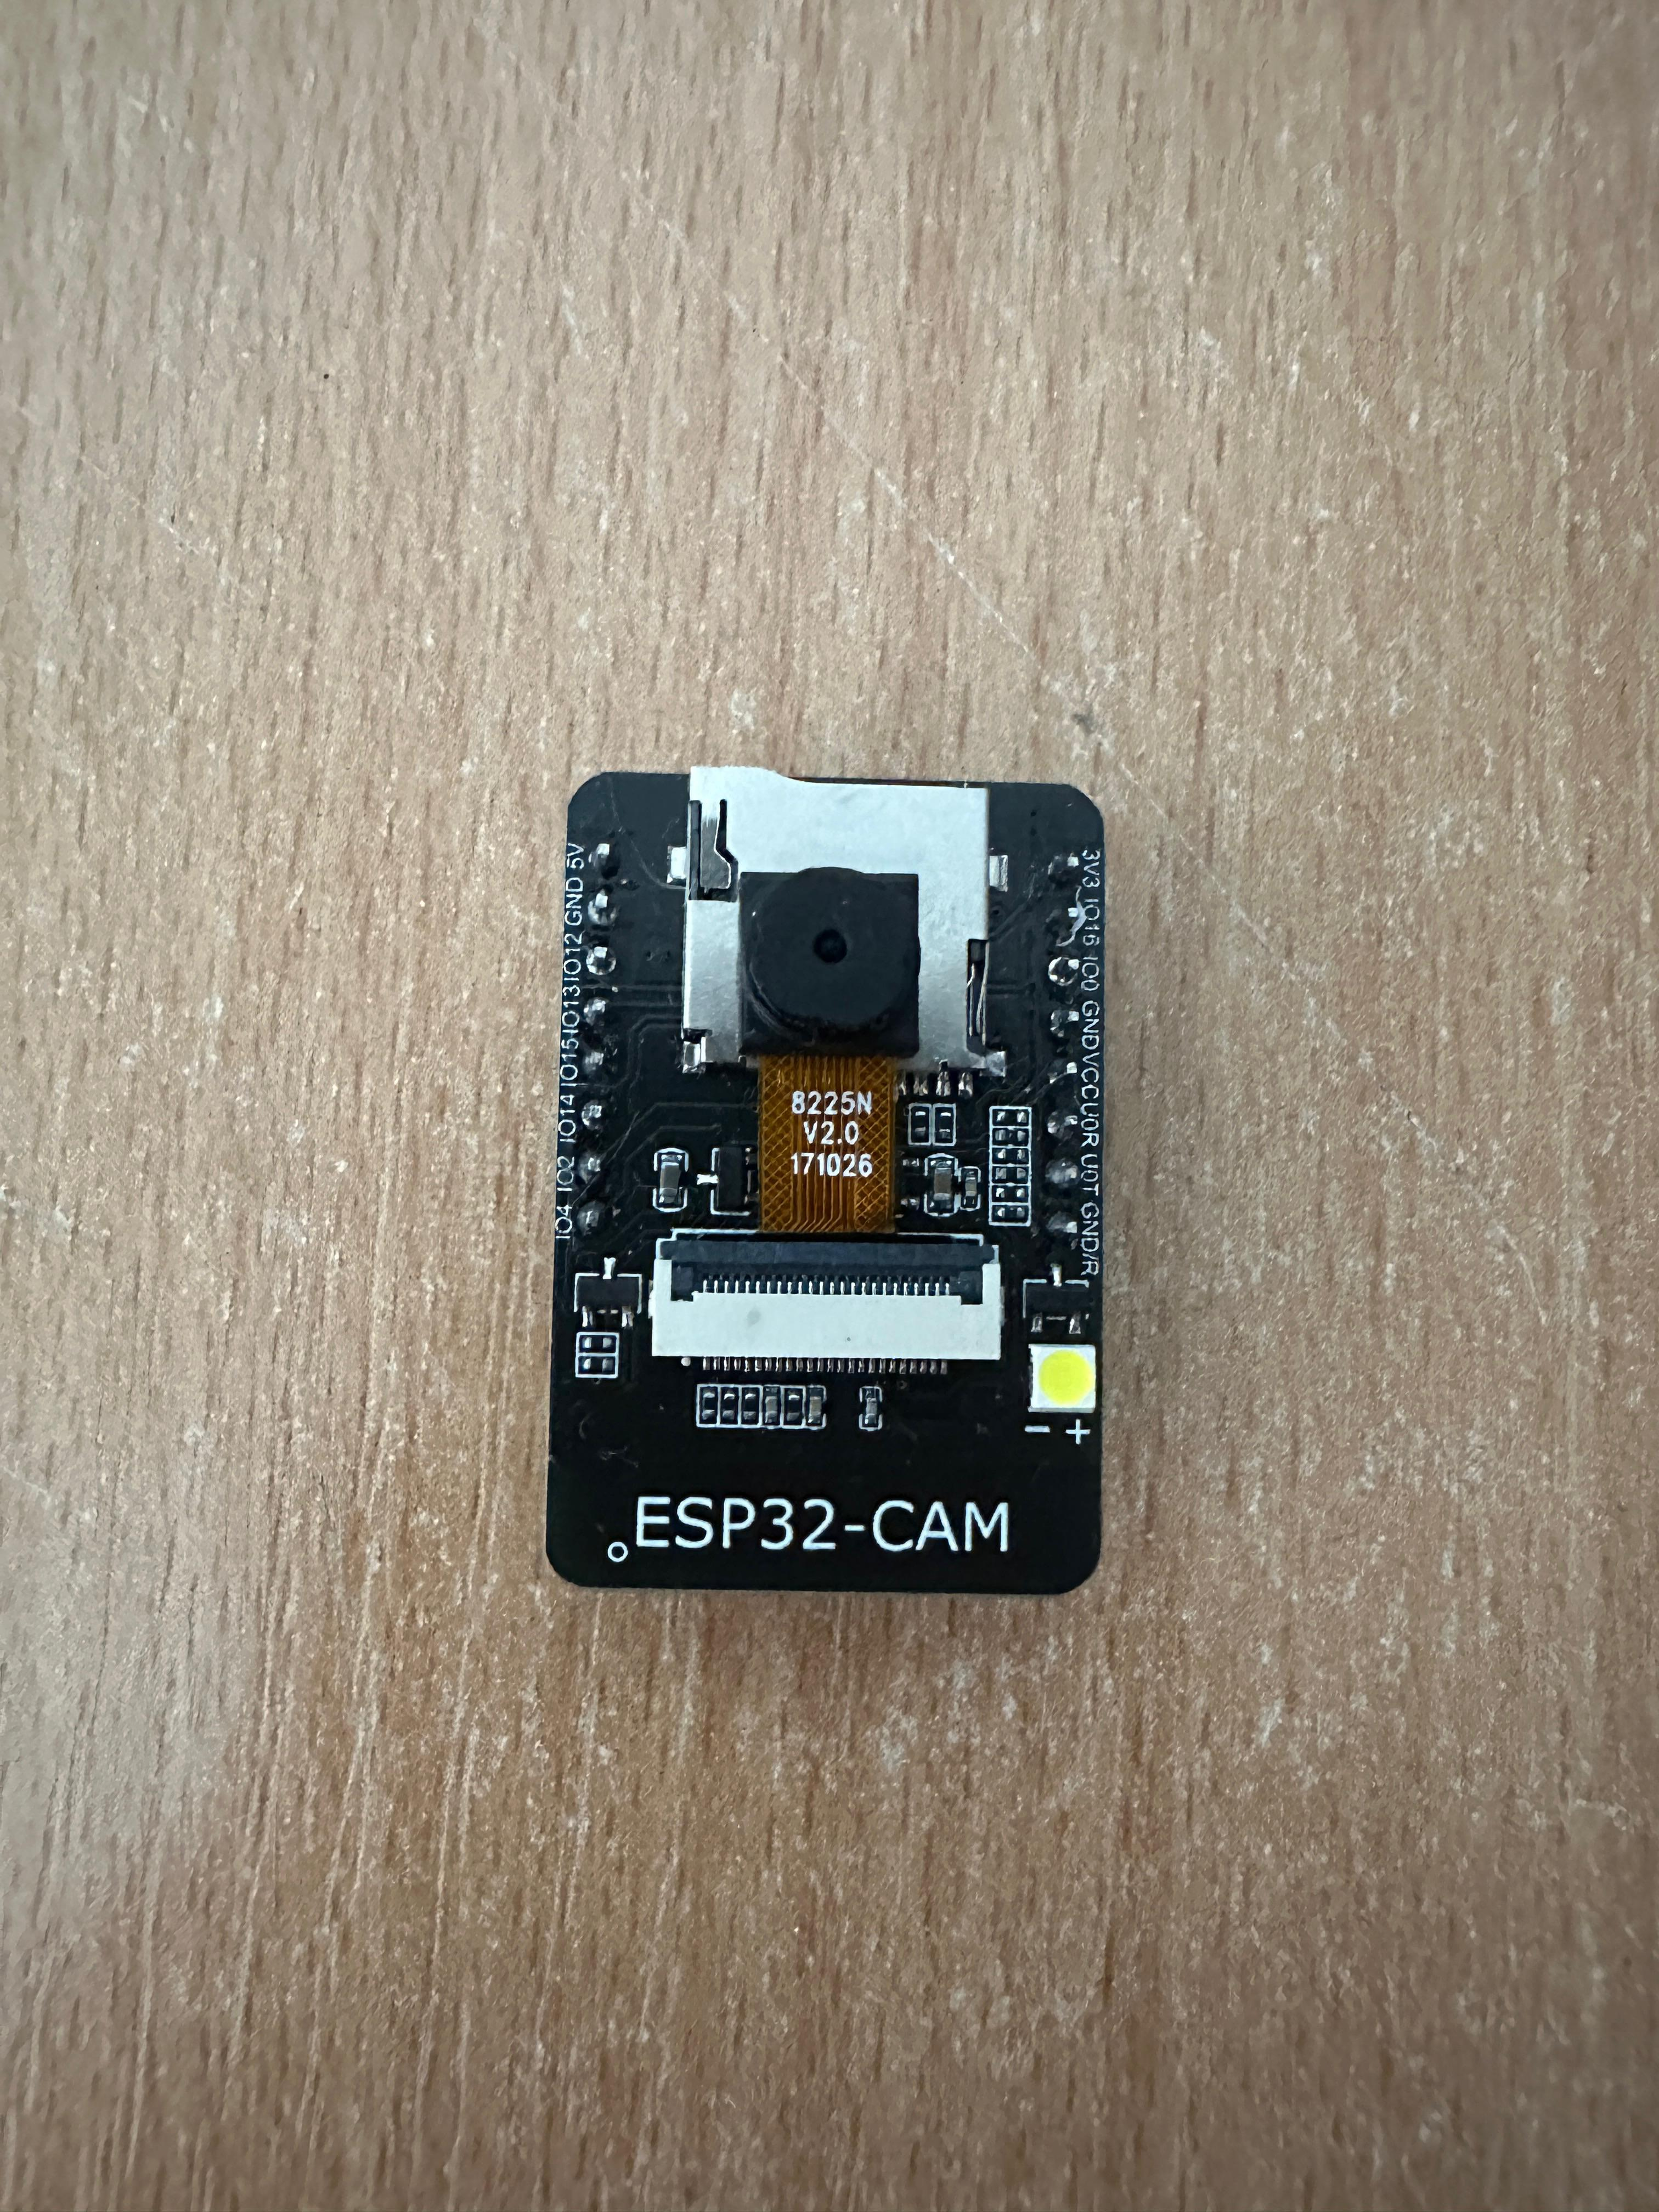
\includegraphics[width=0.4\textwidth]{esp32_cam.jpg}
    \caption{Modul ESP32-CAM}
    \label{fig:esp32_cam}
\end{figure}
    \newpage
    \vspace*{1cm}
    \item \textbf{Motor servo MG996R}: Acesta este un motor servo puternic, utilizat pentru deschiderea ușii sau a sertarului, ideal pentru aplicații care necesită cuplu ridicat și rezistență la șocuri.
    \begin{itemize}
        \item \textbf{Cuplu maxim:} 9.4 kgf·cm (la 4.8V) și 11 kgf·cm (la 6V).
        \item \textbf{Viteză:} 0.17 sec/60° (la 4.8V) și 0.14 sec/60° (la 6V).
        \item \textbf{Tensiune de operare:} 4.8V - 7.2V.
        \item \textbf{Curent în funcționare:} 500 mA.
        \item \textbf{Curent de blocare:} 2.5 A (la 6V).
        \item \textbf{Lățime bandă moartă:} 5 μs.
        \item \textbf{Design:} Stabil și rezistent la șocuri, cu rulmenți dubli.
        \item \textbf{Dimensiuni:} 40.7 × 19.7 × 42.9 mm.
        \item \textbf{Greutate:} 55 g.
        \item \textbf{Alimentare și conexiuni:}
            \begin{itemize}
                \item Firul roșu (VCC): conectat la 5V.
                \item Firul maro (GND): conectat la GND.
                \item Firul galben (PWM): conectat la pinul 10 pe Arduino.
            \end{itemize}
    \end{itemize}
    \begin{figure}[H]
    \centering
    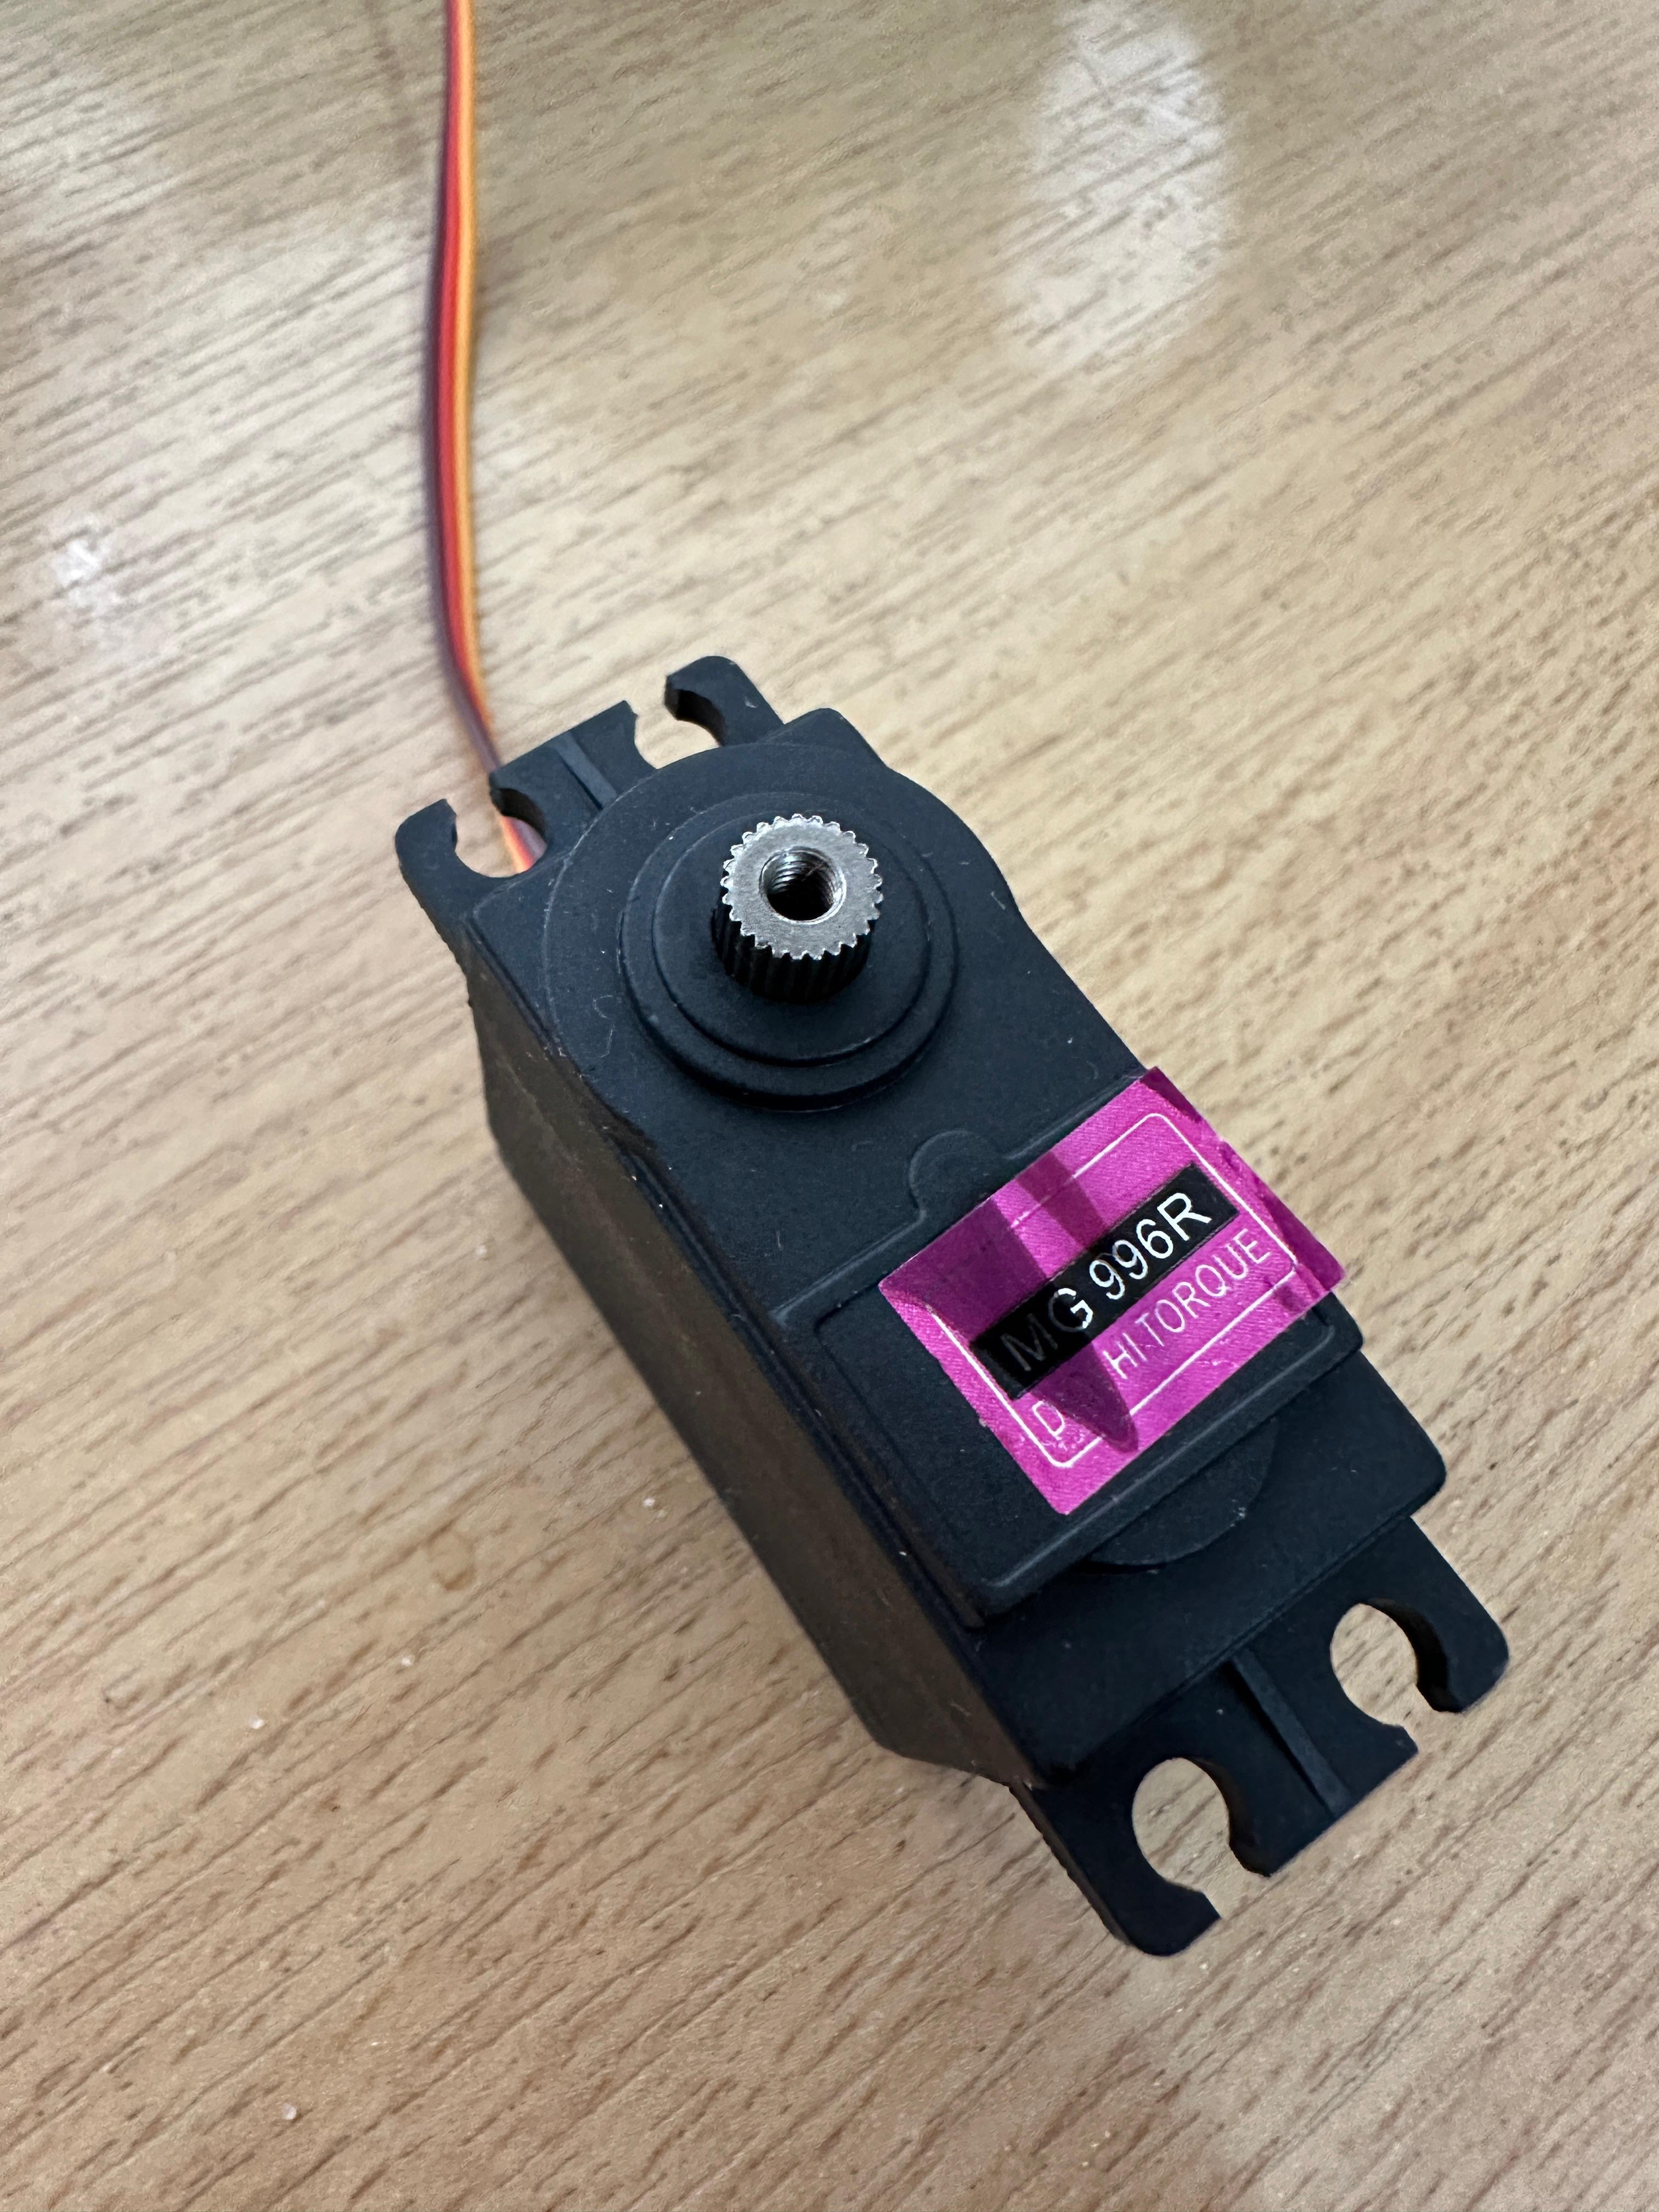
\includegraphics[width=0.4\textwidth]{servo_motor.jpg}
    \caption{Servomotor}
    \label{fig:esp32_cam}
\end{figure}

    \item \textbf{LCD 16x2 cu I2C}: Este utilizat pentru a oferi feedback vizual utilizatorului, afișând mesaje precum "Autorizat" sau "Respins".
    \newpage
    \vspace*{1cm}
    \begin{itemize}
        \item Tip: LCD alfanumeric 16x2 (16 caractere, 2 linii).
        \item Interfață: I2C (reducerea numărului de pini necesari).
        \item Tensiune de alimentare: 5V.
        \item Pini:
            \begin{itemize}
                \item VCC: conectat la 5V pe Arduino.
                \item GND: conectat la GND pe Arduino.
                \item SDA: conectat la pinul analogic A4.
                \item SCL: conectat la pinul analogic A5.
            \end{itemize}
    \end{itemize}
    \begin{figure}[H]
    \centering
    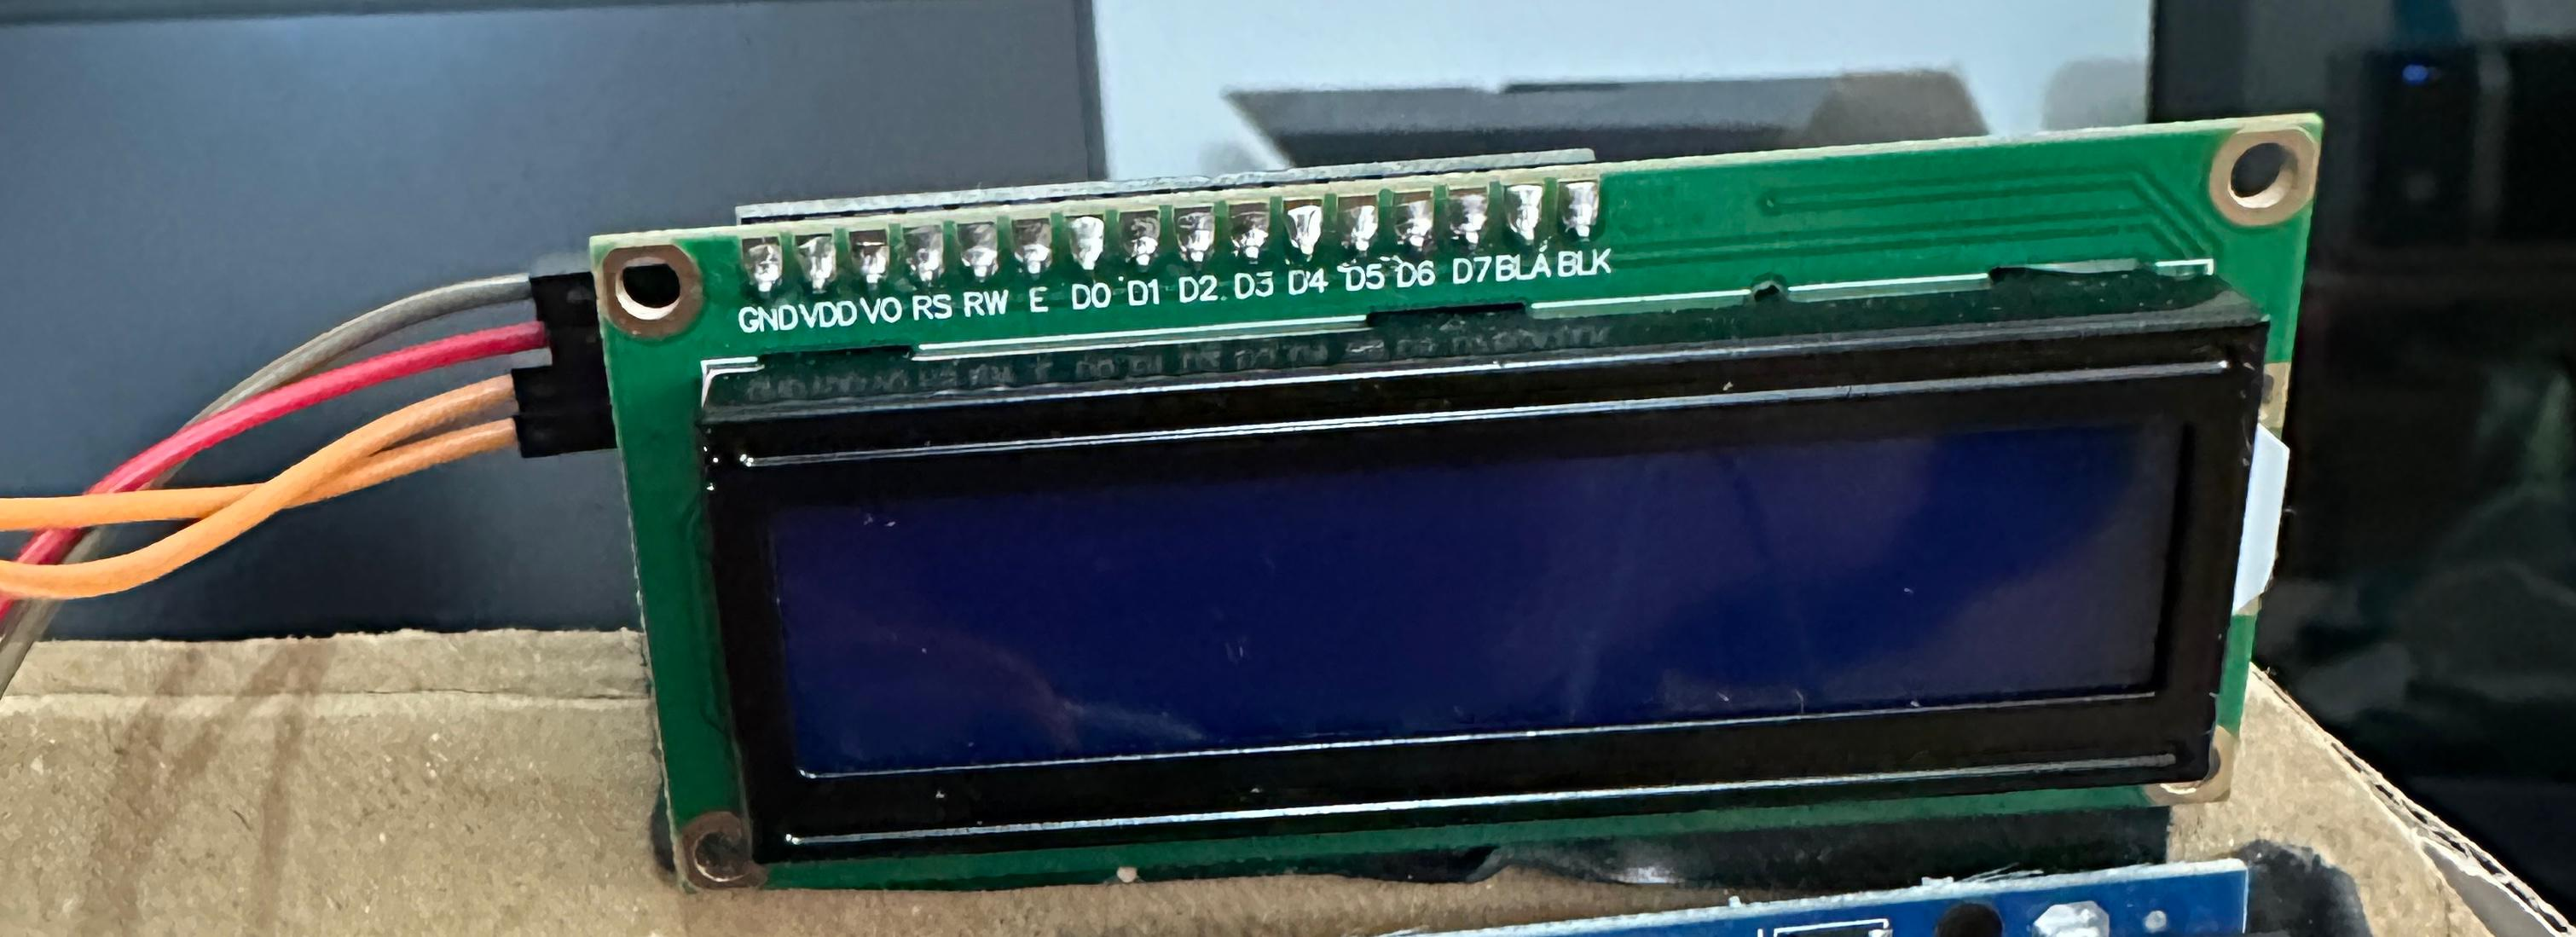
\includegraphics[width=0.6\textwidth]{lcd_i2c.jpg}
    \caption{Lcd I2C}
    \label{fig:lcd}
\end{figure}

    \item \textbf{LED}: Utilizat pentru a indica starea accesului.
    \begin{itemize}
        \item Anodul (piciorul lung): conectat la un pin digital printr-o rezistență (220 ohmi recomandată).
        \item Catodul (piciorul scurt): conectat la GND.
        \item Culoare: Verde pentru acces autorizat, roșu pentru acces respins.
    \end{itemize}
    \begin{figure}[H]
    \centering
    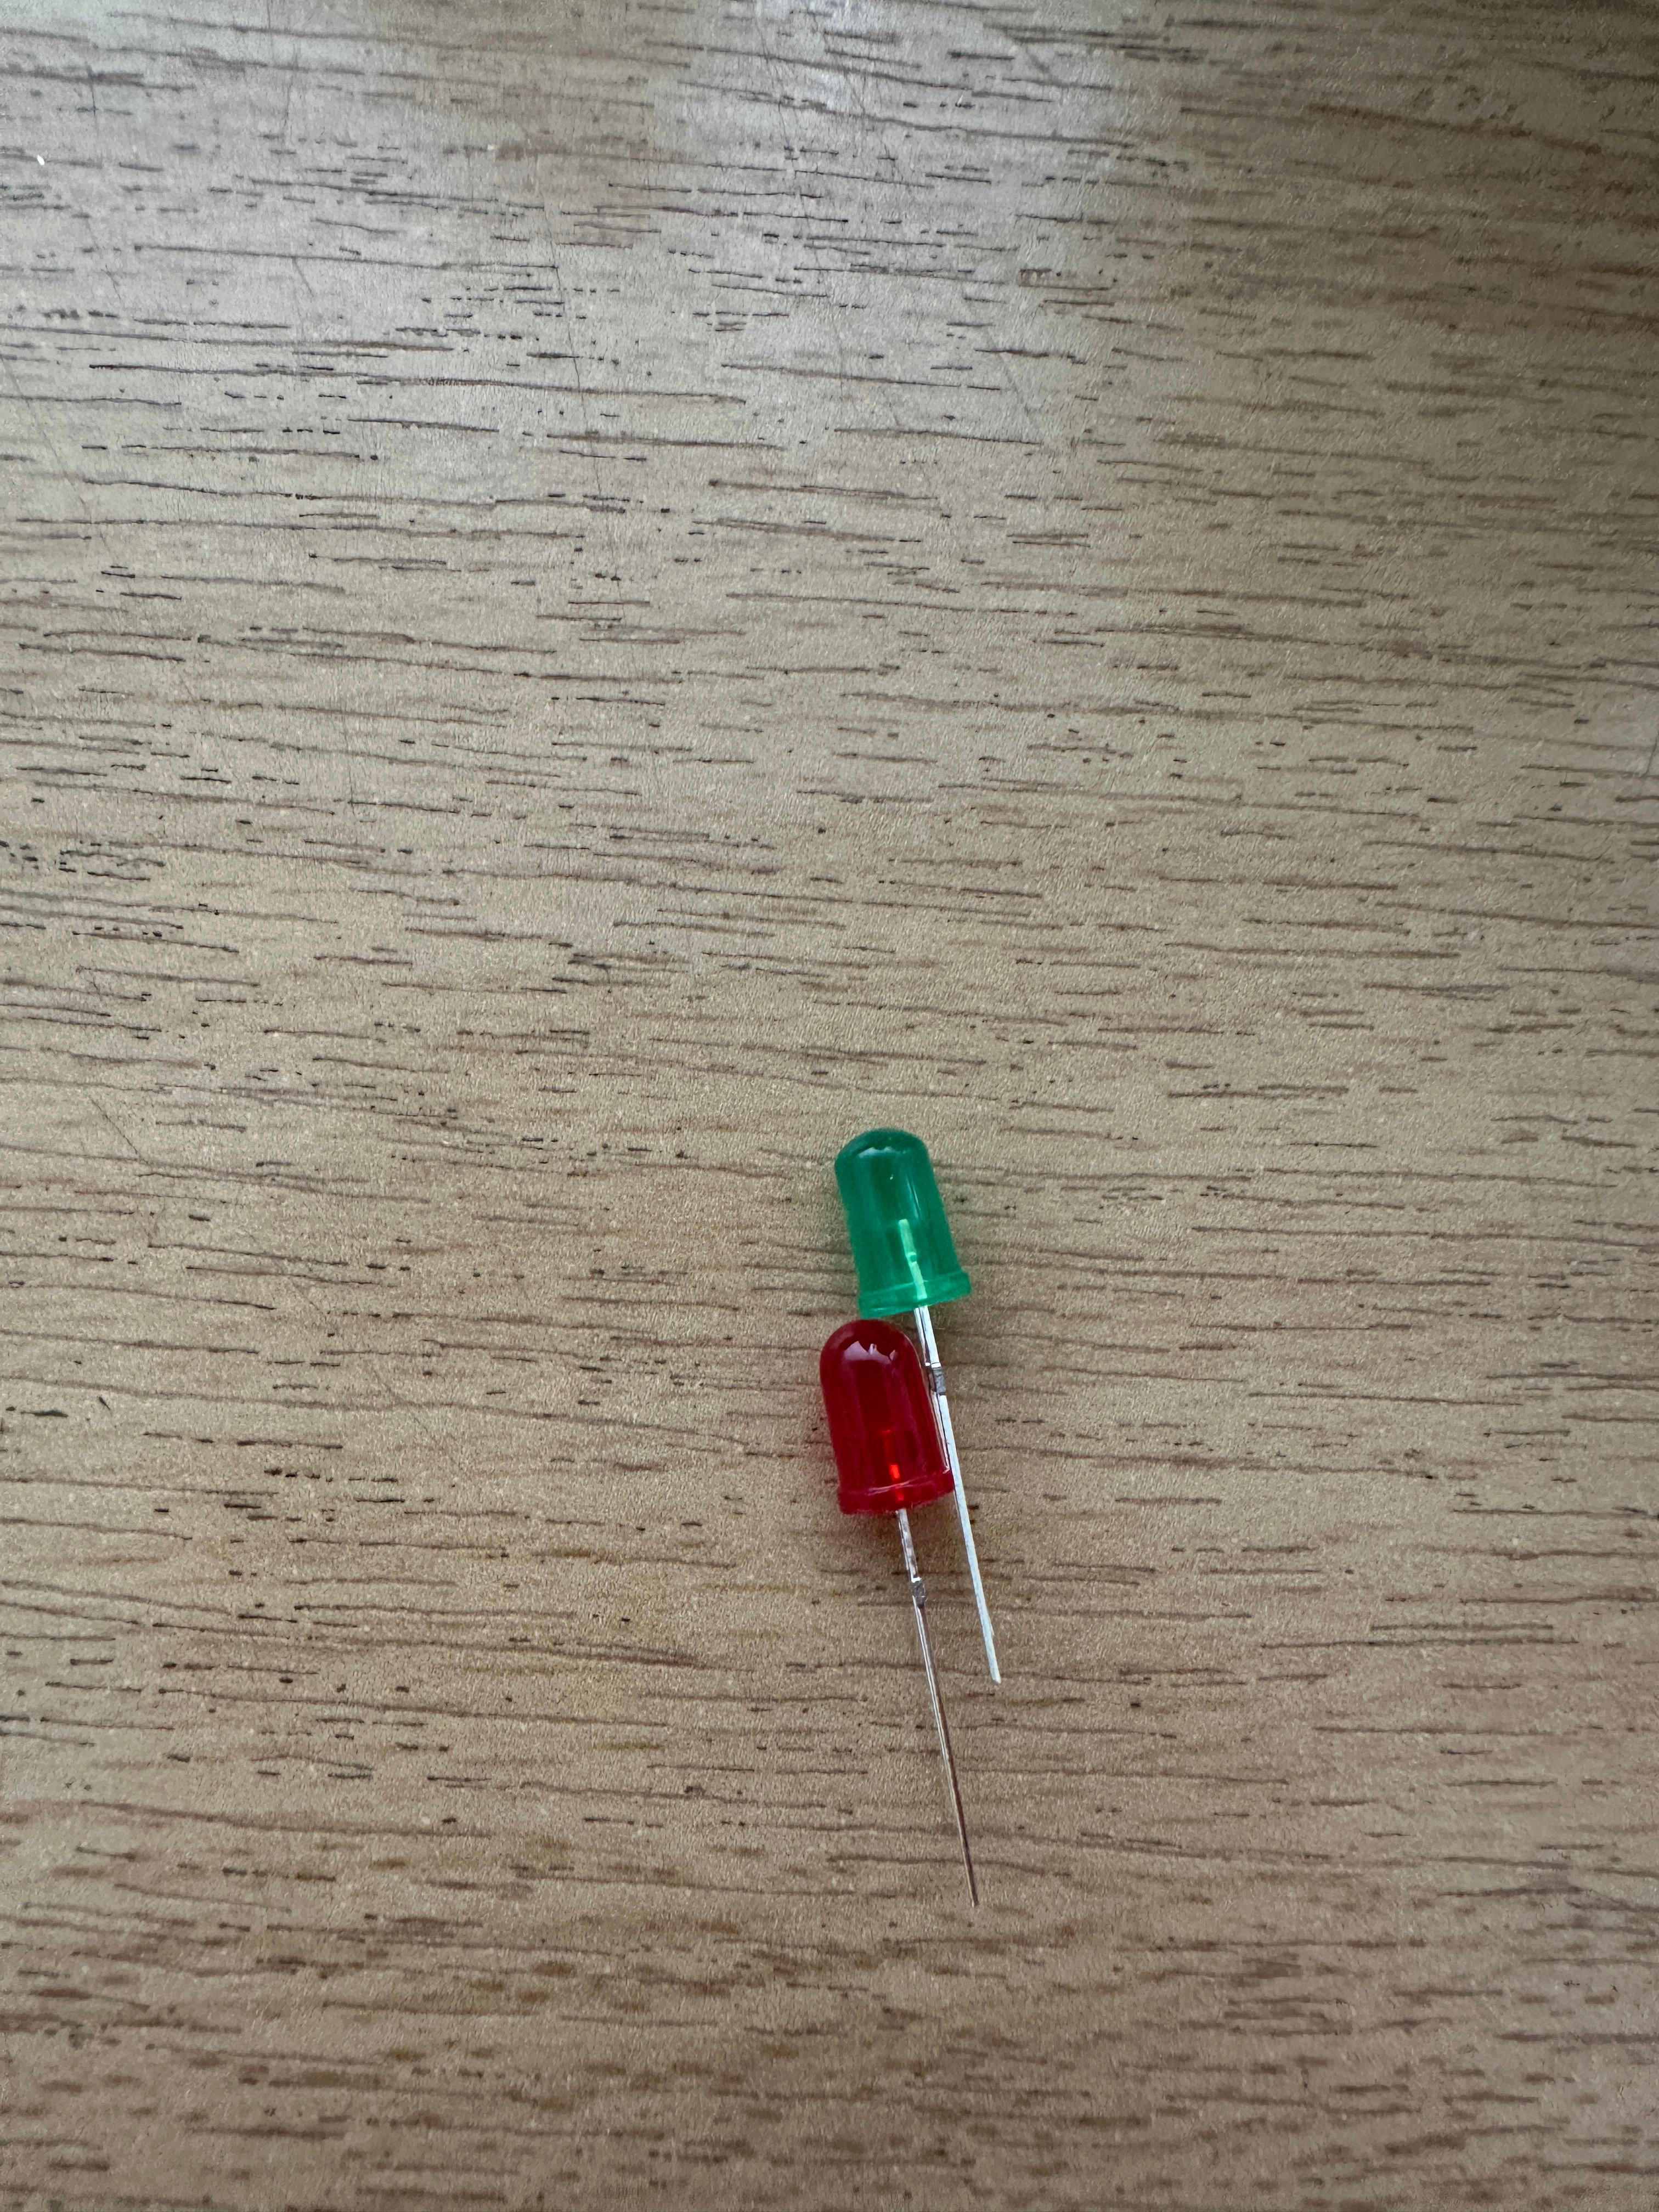
\includegraphics[width=0.3\textwidth]{leds.jpg}
    \caption{Led}
    \label{fig:led}
\end{figure}
\newpage
\vspace*{1cm}

    \item \textbf{Potentiometru:} Utilizat pentru ajustarea contrastului LCD-ului sau a intensității LED-urilor.
    \begin{itemize}
    \vspace*{1cm}
        \item Tensiune de operare: 0-5V.
        \item Conexiuni:
            \begin{itemize}
                \item Terminalul 1 (sau 2): conectat la 5V sau GND.
                \item Wiper-ul (pinul din centru): conectat la A0 pe Arduino.
            \end{itemize}
    \end{itemize}
    \begin{figure}[H]
    \centering
    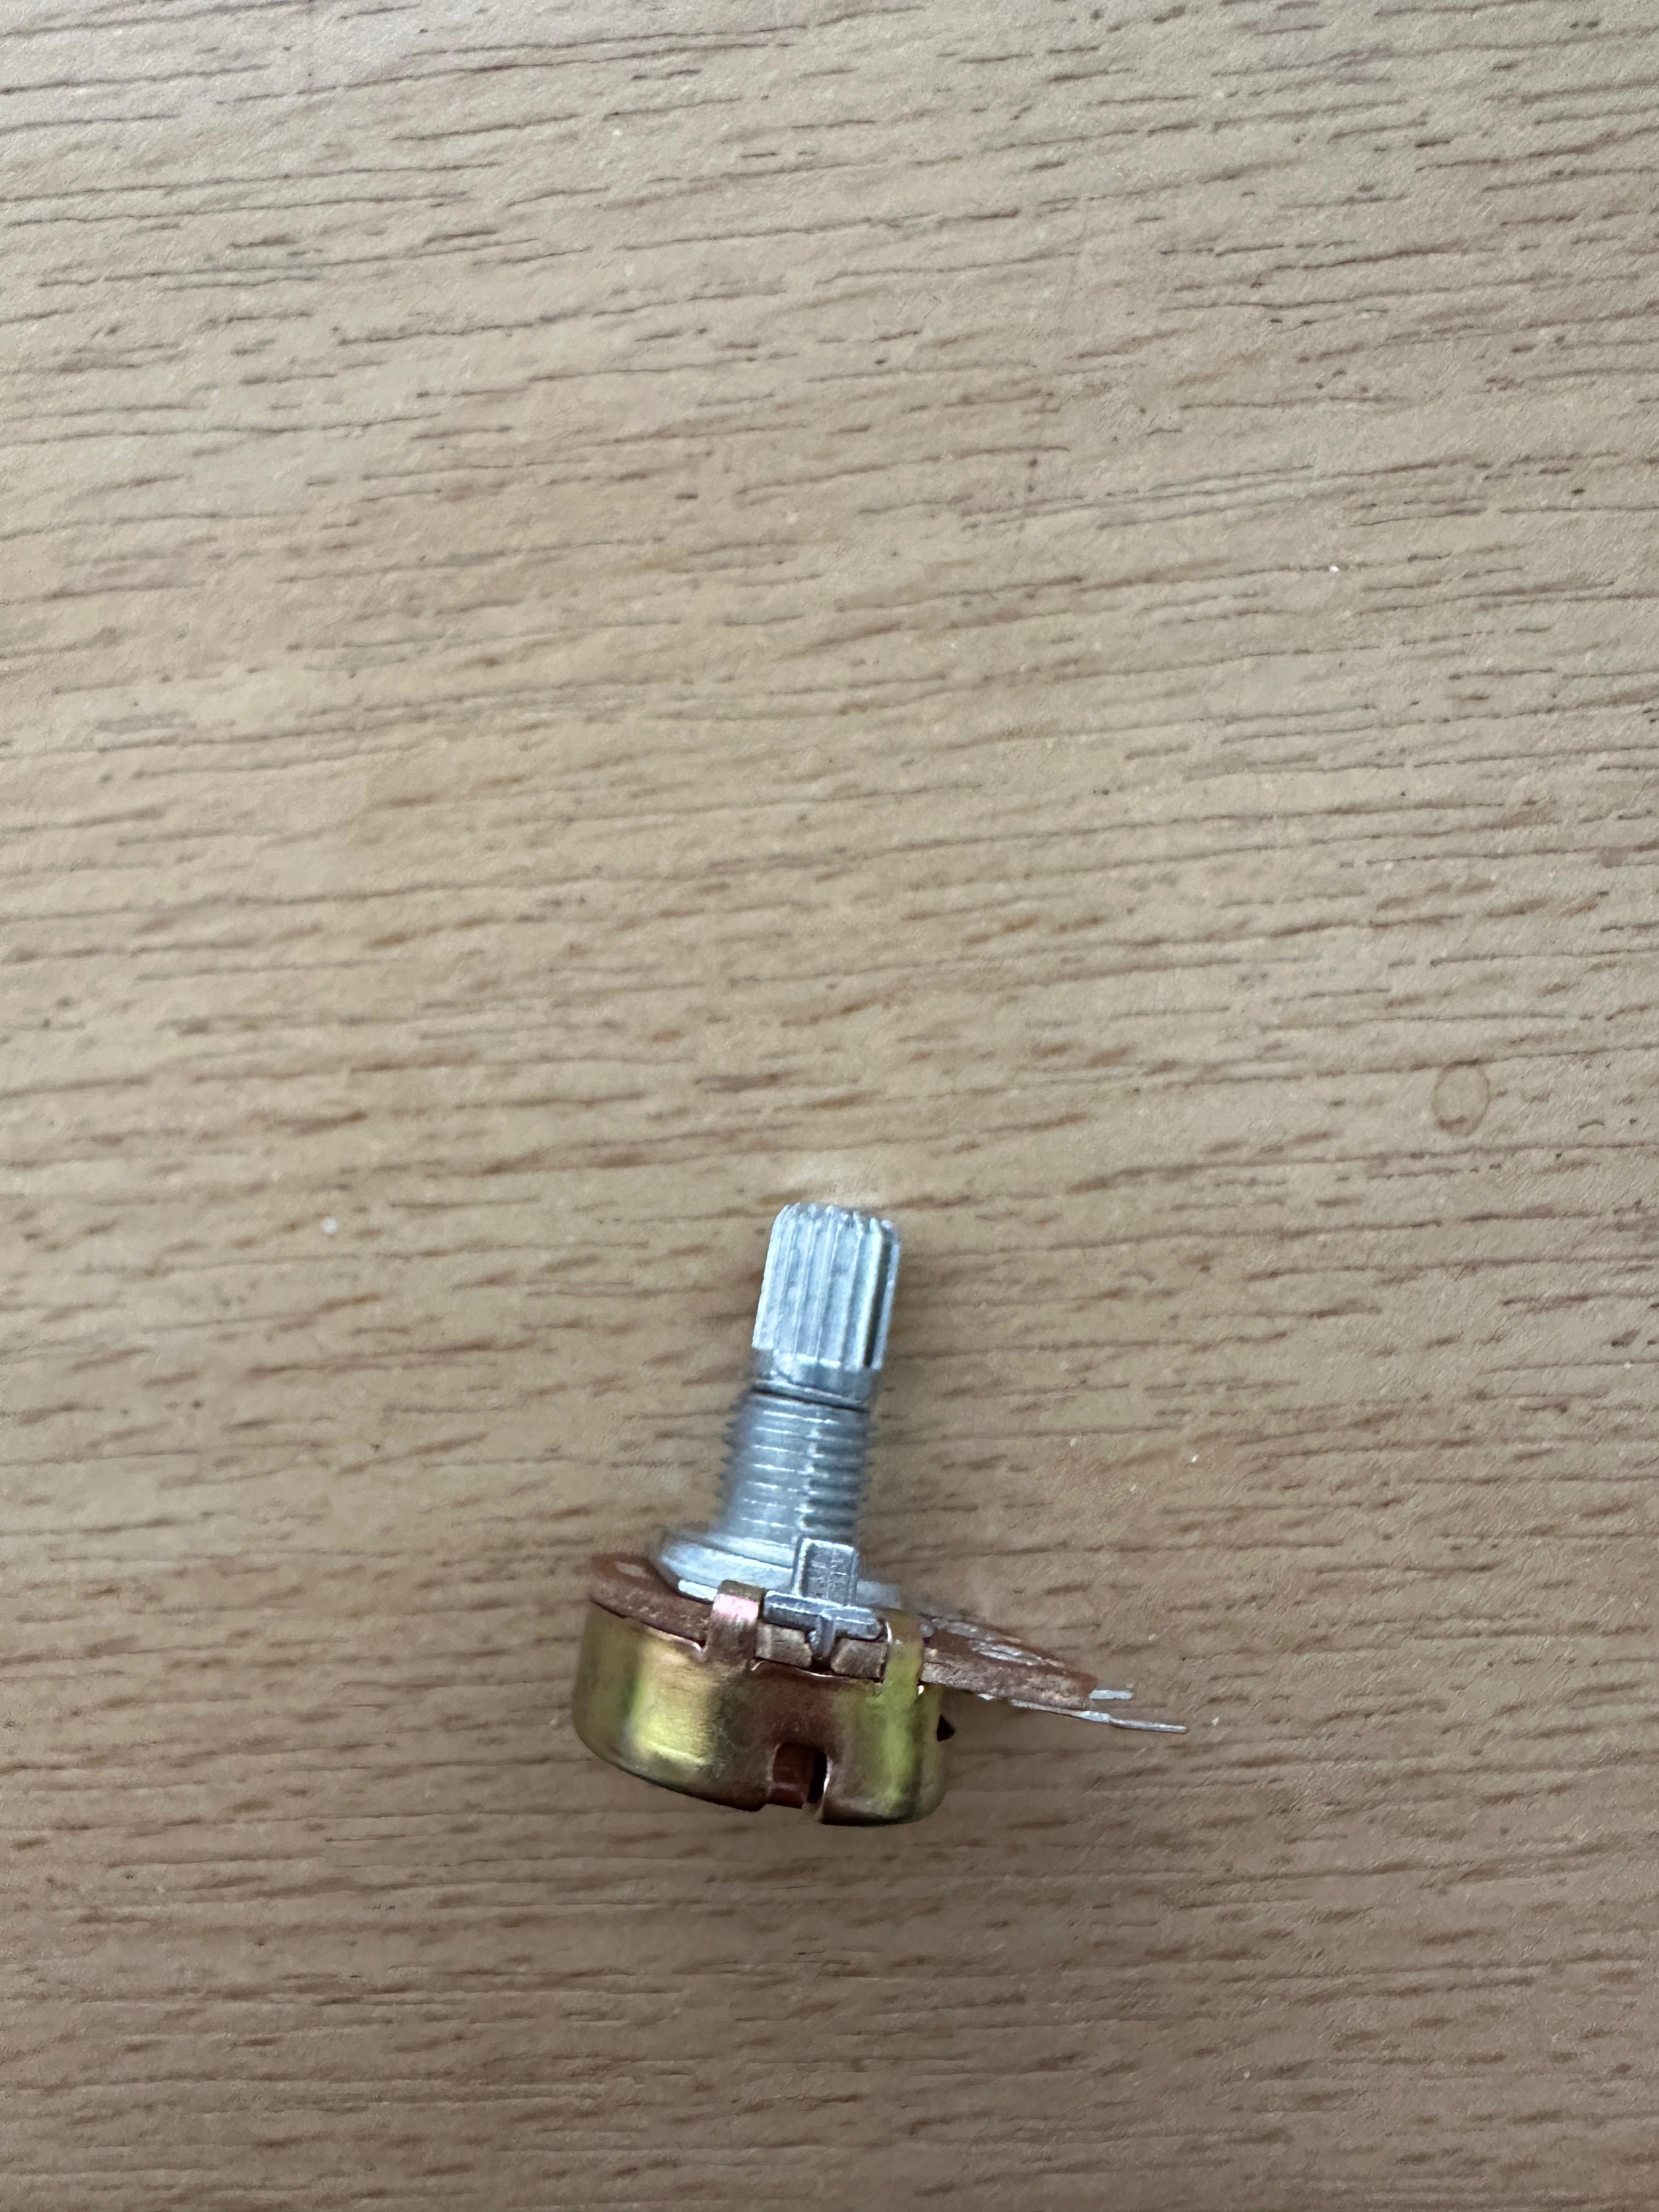
\includegraphics[width=0.4\textwidth]{potentiometru.jpg}
    \caption{Potentiometru}
    \label{fig:potentiometru}
\end{figure}
    \item \textbf{BreadBoard:} Placă de prototipare utilizată pentru conectarea și testarea componentelor hardware fără lipire.
    \begin{itemize}
        \item Dimensiuni: disponibile în diverse formate (ex. 400 sau 830 de pini).
        \item Alimentare: permite conectarea surselor de alimentare externe la șinele dedicate (+ și -).
        \item Conectivitate: orificiile sunt aranjate pentru conectarea rapidă a cablurilor și componentelor.
        \item Utilizare: ideală pentru prototiparea rapidă și modificarea conexiunilor hardware.
    \end{itemize}
    \begin{figure}[H]
    \centering
    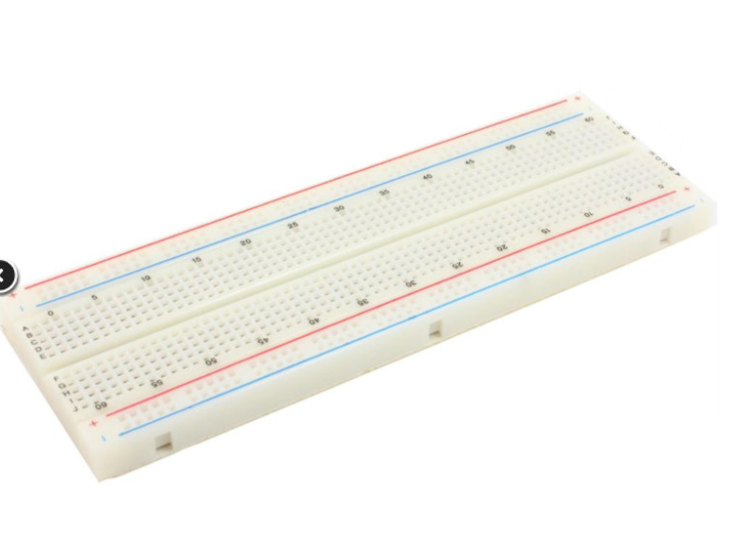
\includegraphics[width=0.4\textwidth]{breadboard.png}
    \caption{BreadBoard}
    \label{fig:breadboard}
\end{figure}

    \item \textbf{Modul sursă de alimentare pentru BreadBoard (5V - 3.3V):}
    \begin{itemize}
        \item \textbf{Intrare:}
            \begin{itemize}
                \item Alimentare prin mufă DC: 6.5V - 12V.
                \item Alimentare prin port USB: 5V.
            \end{itemize}
        \item \textbf{Ieșire:}
            \begin{itemize}
                \item Tensiuni selectabile: 3.3V și 5V.
                \item Curent maxim: 700 mA.
            \end{itemize}
        \item \textbf{Utilizare:}
            \begin{itemize}
                \item Se plasează pe BreadBoard pentru alimentarea rapidă a componentelor.
                \item Include switch-uri pentru selectarea tensiunii de ieșire (5V sau 3.3V).
                \item Are indicator LED pentru starea alimentării.
            \end{itemize}
    \end{itemize}
\end{itemize}
\begin{figure}[H]
    \centering
    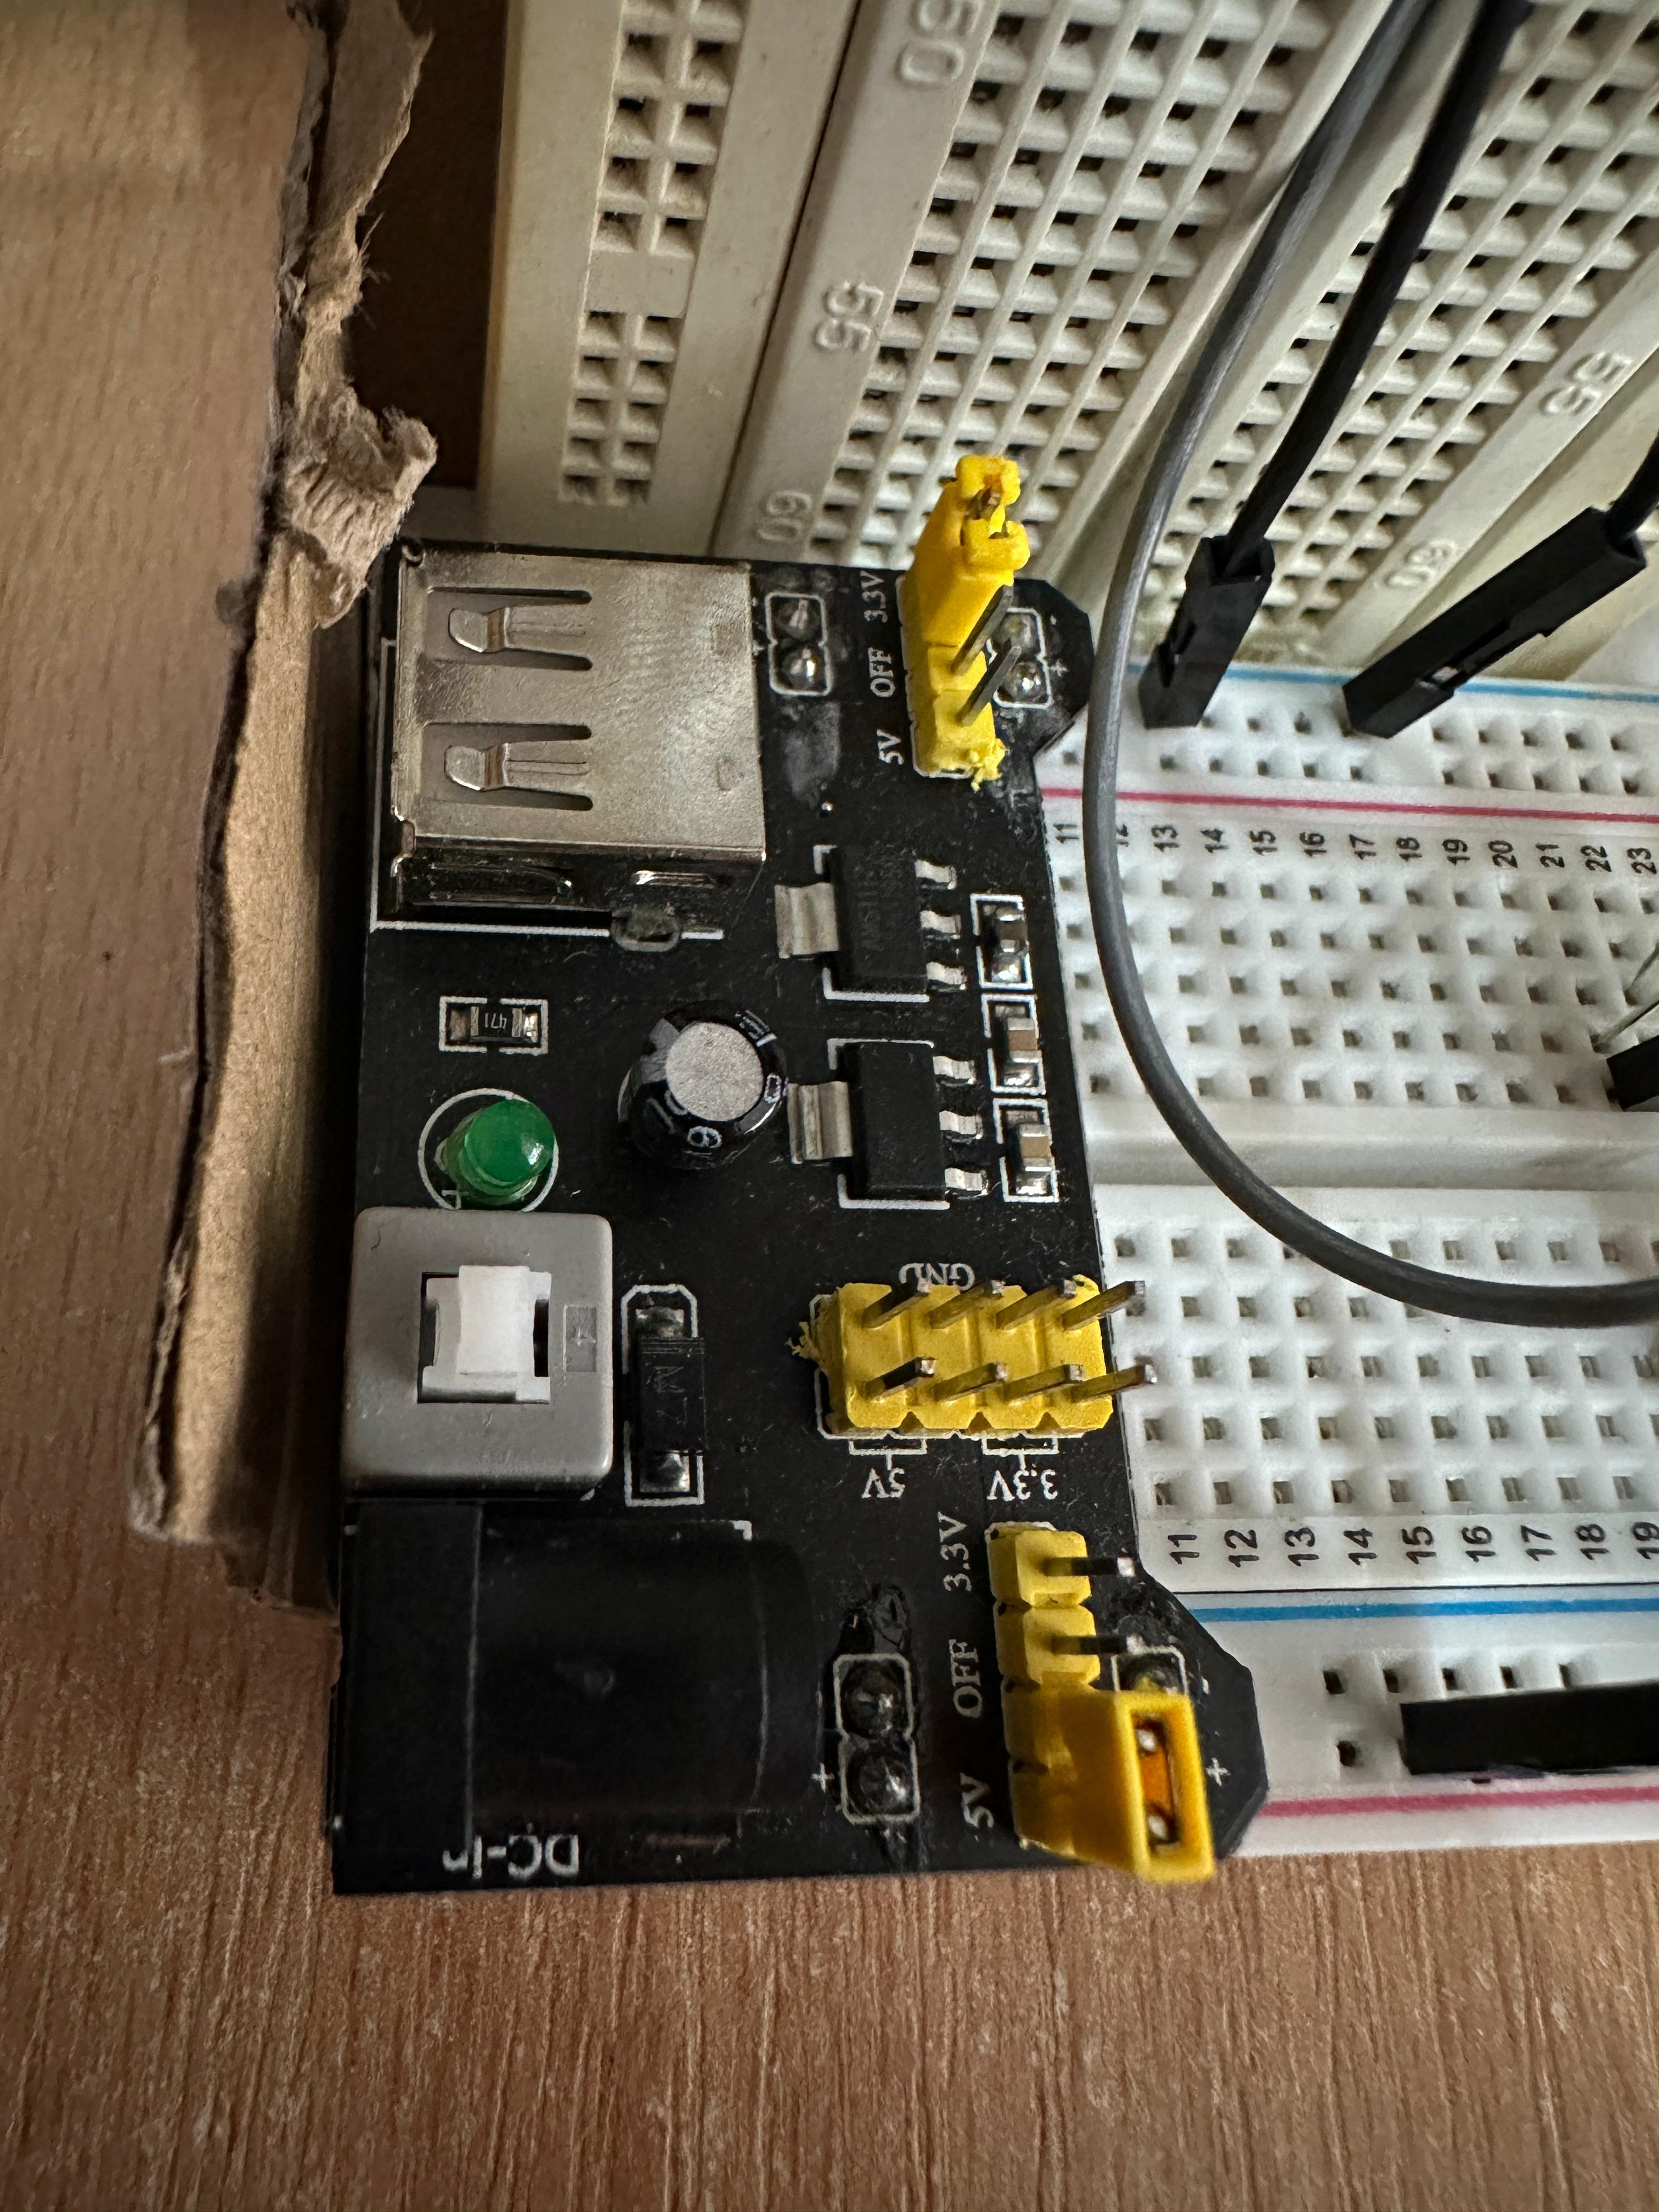
\includegraphics[width=0.4\textwidth]{power_supply.jpg}
    \caption{Modul sursă de alimentare}
    \label{fig:sursa}
\end{figure}

\chapter{Descrierea lucrării}

\section{Introducere}
Lucrarea propune realizarea unui sistem de acces controlat bazat pe recunoaștere facială, utilizând microcontrolerul Arduino Uno și un modul ESP32-CAM pentru capturarea și procesarea imaginilor. Acest sistem integrează mai multe componente hardware și software pentru a oferi o soluție eficientă și sigură de acces autorizat. Proiectul este implementat astfel încât să poată fi folosit în diverse aplicații, cum ar fi controlul accesului la uși, sertare sau alte spații securizate.

\section{Structura sistemului}
Sistemul este format din următoarele componente principale:
\begin{itemize}
    \item \textbf{ESP32-CAM}: Capturarea imaginii feței utilizatorului și transmiterea acesteia către un script Python pentru procesare.
    \item \textbf{Arduino Uno}: Microcontrolerul principal care gestionează semnalele de intrare/ieșire și controlează funcționarea componentelor hardware (servo, LED-uri, LCD).
    \item \textbf{Motor servo MG996R}: Controlează deschiderea mecanismului fizic (ușă sau sertar) în cazul în care accesul este autorizat.
    \item \textbf{LCD 16x2 cu I2C}: Afișează mesajele relevante utilizatorului, cum ar fi "Autorizat" sau "Respins".
    \item \textbf{LED-uri}: Indică rapid starea accesului (verde pentru acces autorizat, roșu pentru acces refuzat).
    \item \textbf{Modul sursă de alimentare pentru BreadBoard}: Oferă alimentare stabilă pentru toate componentele hardware.
\end{itemize}
\newpage
\vspace*{1cm}
\section{Fluxul de funcționare al sistemului}
Procesul de funcționare poate fi descris astfel:
\begin{enumerate}
    \item \textbf{Capturarea imaginii:} Modulul ESP32-CAM captează imaginea feței utilizatorului și o trimite către un PC pentru procesare prin intermediul unui script Python.
    \item \textbf{Procesarea imaginii:} Scriptul Python preia imaginea, o compară cu imaginile stocate în baza de date și decide dacă accesul este autorizat sau respins.
    \item \textbf{Transmiterea rezultatului:} Rezultatul verificării (autorizat sau respins) este trimis către Arduino prin protocol UART.
    \item \textbf{Controlul mecanismului:} Arduino interpretează rezultatul:
    \begin{itemize}
        \item Dacă accesul este autorizat, motorul servo este activat pentru a deschide ușa/sertarul, iar LED-ul verde se aprinde și pe ecranul LCD apare mesajul "Acces permis".
        \item Dacă accesul este respins, LED-ul roșu se aprinde și pe ecranul LCD apare mesajul "Acces respins".
    \end{itemize}
    \item \textbf{Feedback vizual:} Mesajele de stare sunt afișate pe LCD 16x2, iar LED-urile indică rapid starea accesului.
\end{enumerate}

\section{Interacțiunea hardware-software}
Sistemul combină avantajele hardware-ului (Arduino și ESP32-CAM) cu flexibilitatea oferită de software-ul Python pentru procesarea imaginilor:
\begin{itemize}
    \item \textbf{Arduino Uno:}
    \begin{itemize}
        \item Gestionează controlul motorului servo prin semnal PWM.
        \item Afișează mesajele pe LCD și controlează LED-urile.
        \item Primește rezultatul procesării imaginii prin UART.
    \end{itemize}
    \item \textbf{ESP32-CAM:}
    \begin{itemize}
        \item Capturează imaginea feței utilizatorului.
        \item Trimite imaginea către scriptul Python printr-un URL generat automat.
    \end{itemize}
    \newpage
    \vspace*{1cm}
    \item \textbf{Script Python:}
    \begin{itemize}
        \item Preia imaginea de la ESP32-CAM.
        \item Procesează imaginea și compară fața utilizatorului cu baza de date.
        \item Trimite rezultatul către Arduino prin comunicare serială (UART).
    \end{itemize}
\end{itemize}
\begin{figure}[H]
    \centering
    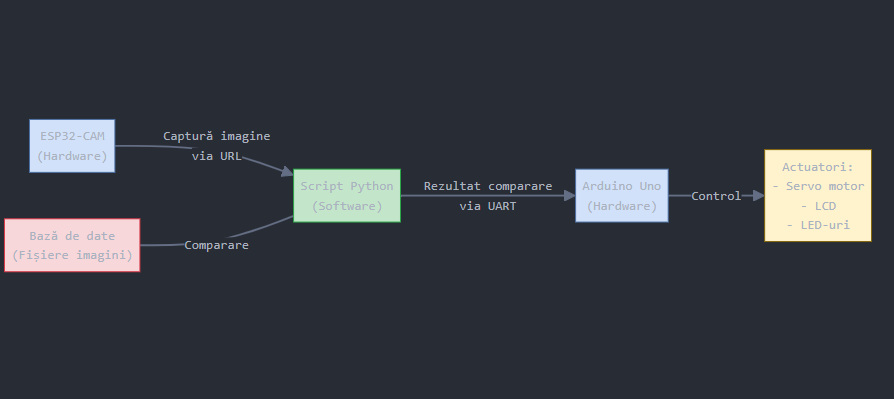
\includegraphics[width=0.8\textwidth]{Schema hardware-software.png}
    \caption{Interacțiunea HW-SW}
    \label{fig:schemahw-sw}
\end{figure}

\section{Programarea pe regiștri}
Controlul precis al motorului servo și al altor periferice este realizat prin programarea registrelor microcontrolerului ATmega328. 
\begin{itemize}
    \item \textbf{Timeri și PWM:} Utilizați pentru a genera semnalul PWM necesar controlului motorului servo.
    \item \textbf{Registre DDR, PORT și PIN:} Folosite pentru configurarea pinilor digitali ca intrări sau ieșiri și pentru citirea sau setarea stării acestora.
\end{itemize}

\section{Avantaje și aplicații}
Sistemul propus oferă următoarele avantaje:
\begin{itemize}
    \item \textbf{Securitate ridicată:} Folosirea recunoașterii faciale reduce riscul accesului neautorizat.
    \item \textbf{Flexibilitate:} Sistemul poate fi adaptat pentru diverse scenarii, cum ar fi controlul accesului la clădiri, dulapuri sau alte spații securizate.
    \item \textbf{Cost redus:} Componentele utilizate sunt accesibile și ușor de integrat.
\end{itemize}
\vspace*{1cm}
\section{Rezumatul lucrării}
Această lucrare demonstrează implementarea unui sistem de acces controlat prin recunoaștere facială, combinând hardware-ul și software-ul pentru a crea un sistem funcțional și eficient. Prin utilizarea registrelor, motorului servo, ESP32-CAM și a scriptului Python, proiectul ilustrează integrarea practică a tehnologiilor moderne în aplicații reale.

\begin{figure}[H]
    \centering
    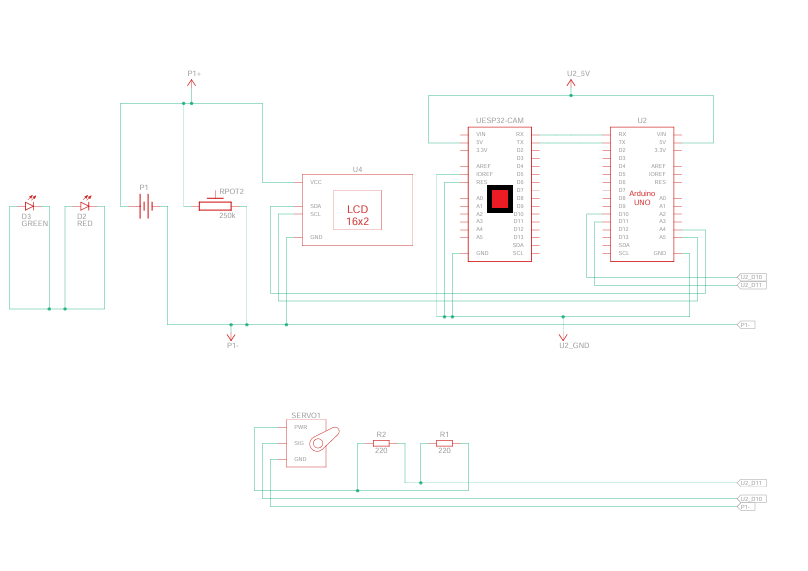
\includegraphics[width=\textwidth, angle=90]{schema_electricaESP.png}
    \caption{Schema electrică}
    \label{fig:schema_electrica}
\end{figure}

\begin{figure}[H]
    \centering
    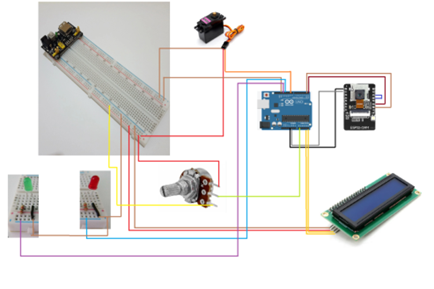
\includegraphics[width=1.3\textwidth, angle=90]{schema_montajESP.png}
    \caption{Schema montaj}
    \label{fig:schema_montaj}
\end{figure}

\newpage
\vspace*{1cm}
Schemele de mai sus prezintă modul în care sunt conectate componentele astfel încat să comunice corect între ele. TX și RX sunt pinii prin care Arduino transmite si recepționează date înspre și dinspre ESP.Semnalul GPIO de pe ESP este necesar pentru programarea ESP-ului și se conectează la GND. După încărcarea codului, firul dintre acești doi pini se exclude pentru a accesa portul serial și a reseta ESP. De asemenea pentru a porni motorul, firul dintre GND si reset trebuie deconectat. 



\chapter{Desfășurarea lucrării - partea 1}

În această secțiune, se va detalia procesul de montare al componentelor hardware utilizate în cadrul proiectului, evidențiind fiecare componentă individual și oferind exemple simple de aplicații pentru studenți, utilizând componentele disponibile.

\section{Arduino Uno}
Placa Arduino Uno este microcontrolerul principal care gestionează logica și semnalele de intrare/ieșire. Aceasta este conectată la celelalte componente pentru a controla funcționarea sistemului.

\begin{figure}[H]
    \centering
    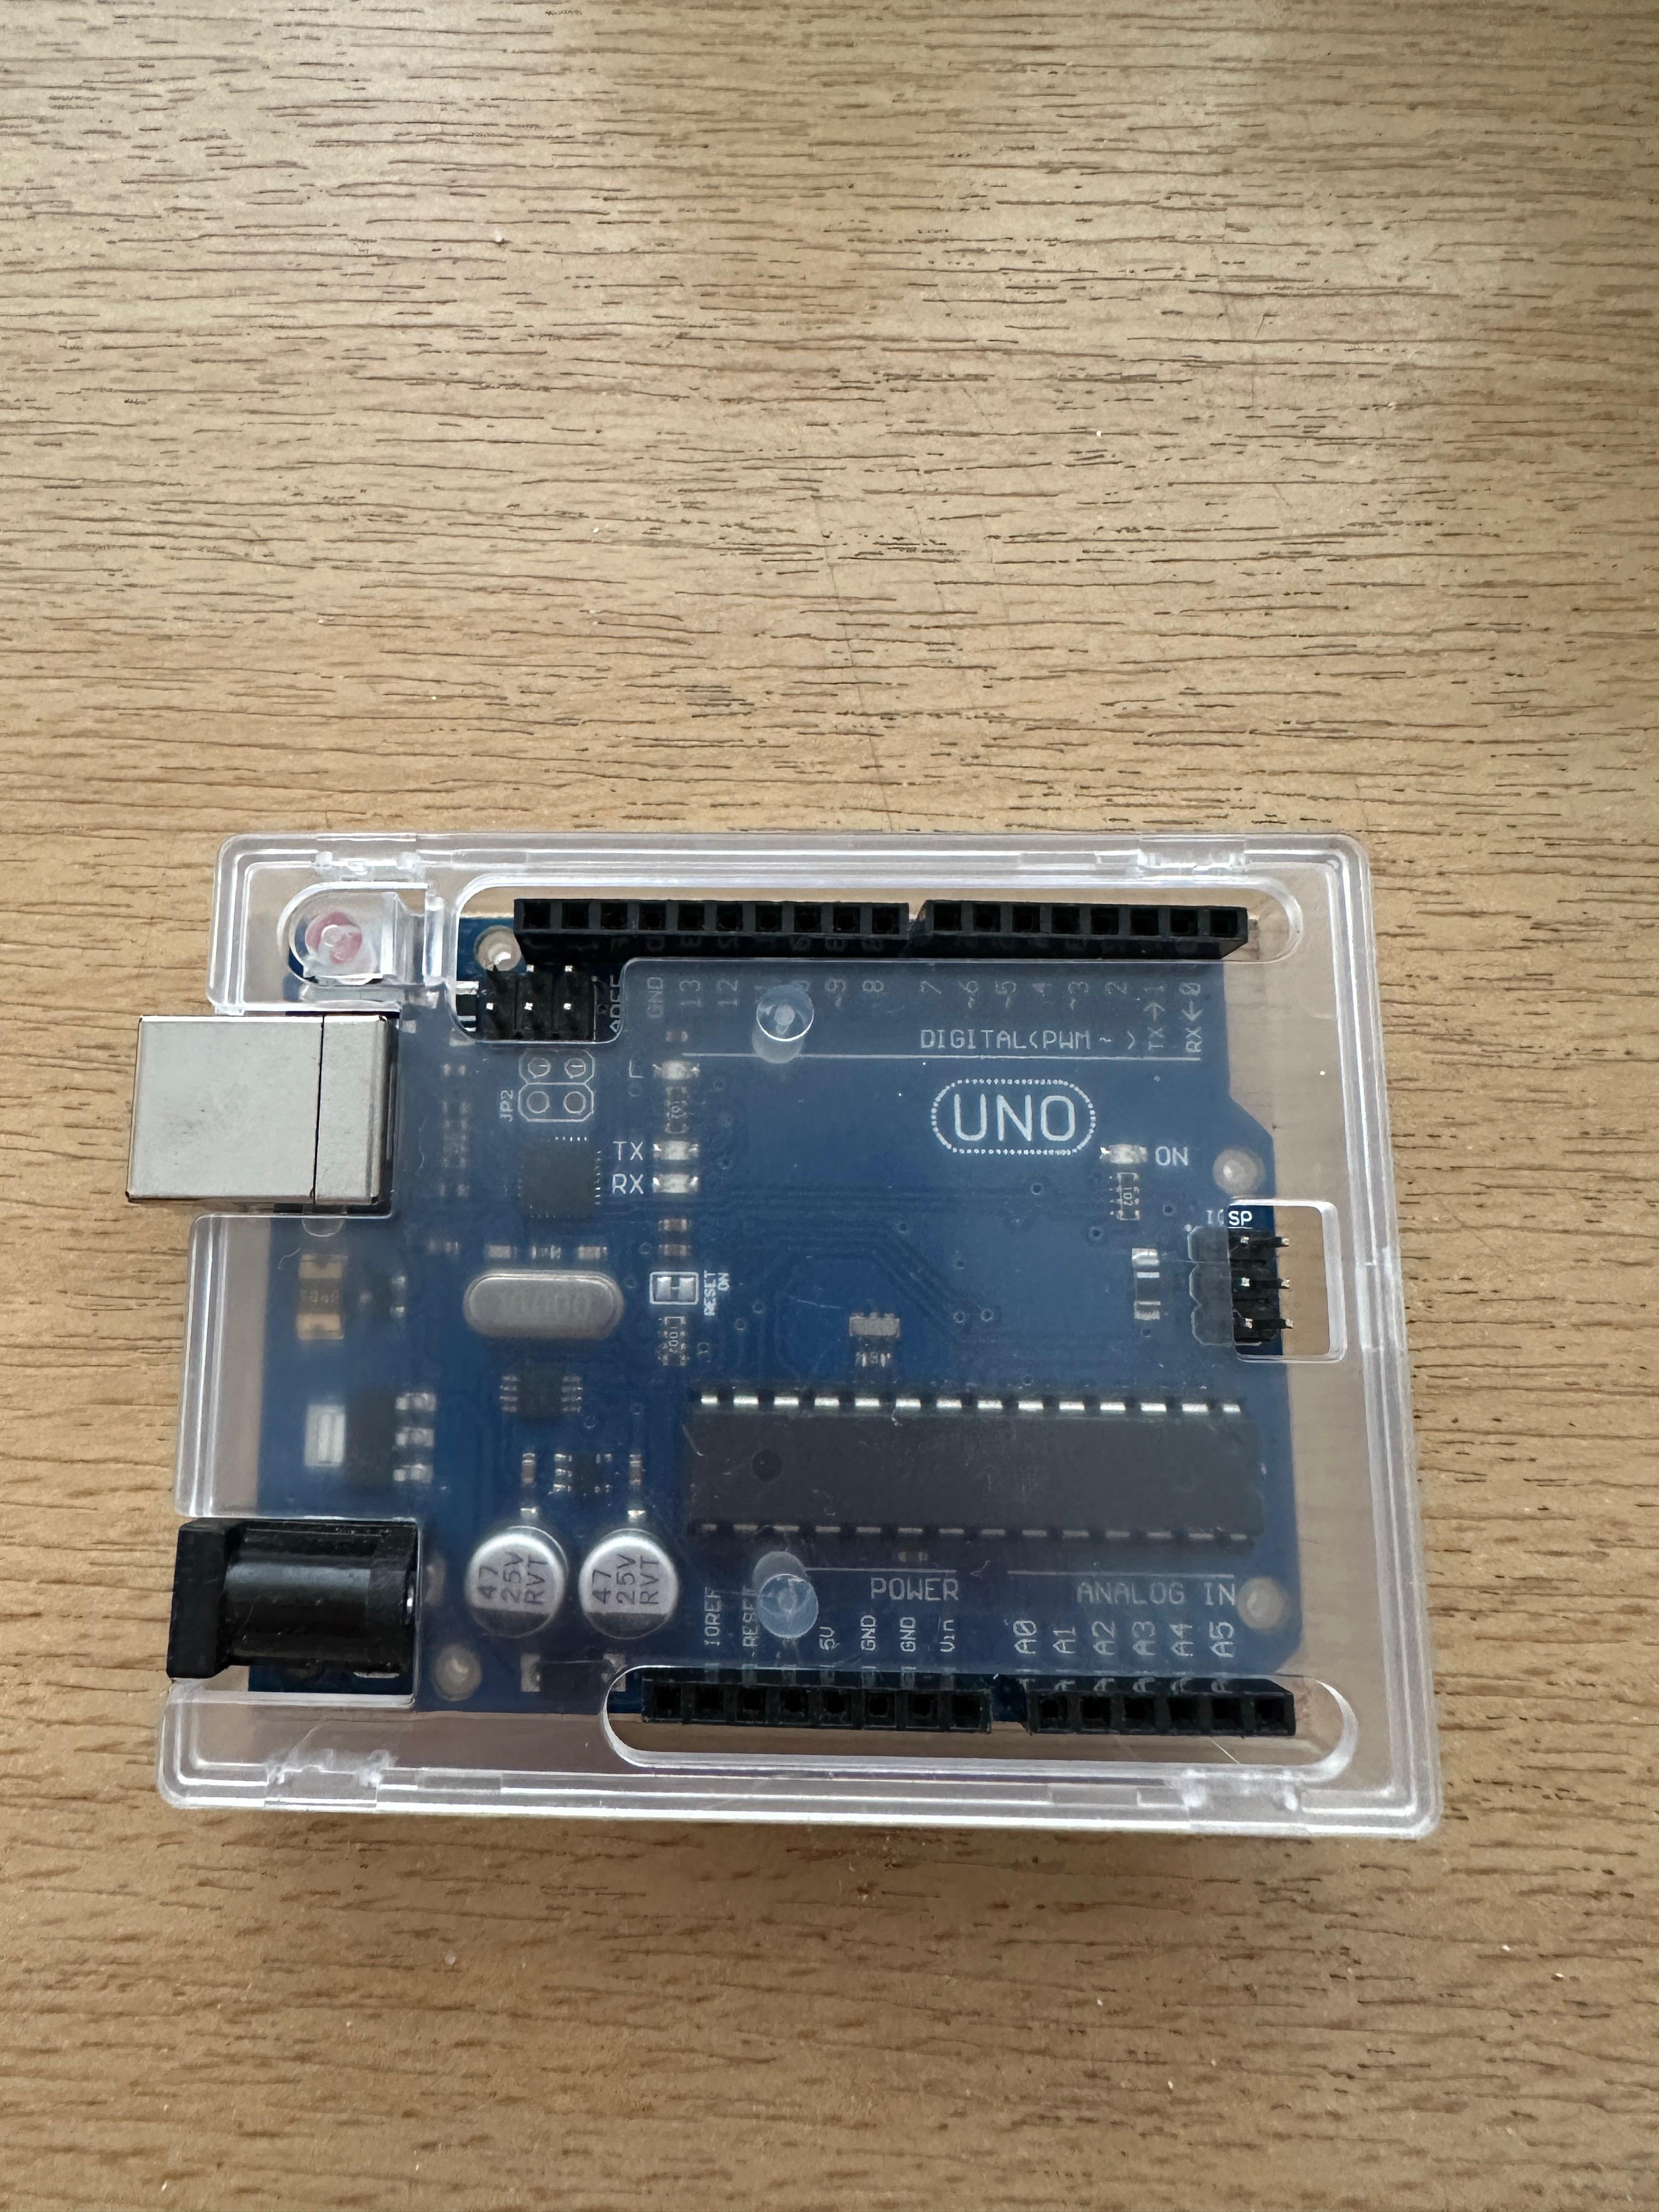
\includegraphics[width=0.4\textwidth]{arduino.jpg}
    \caption{Placa Arduino Uno}
    \label{fig:arduino}
\end{figure}
\newpage
\vspace*{1cm}
\subsection*{Aplicații pentru studenți}
\begin{itemize}
    \item Controlul unui LED pentru a învăța cum să folosească pinii digitali ai Arduino.

    \begin{figure}[H]
    \centering
    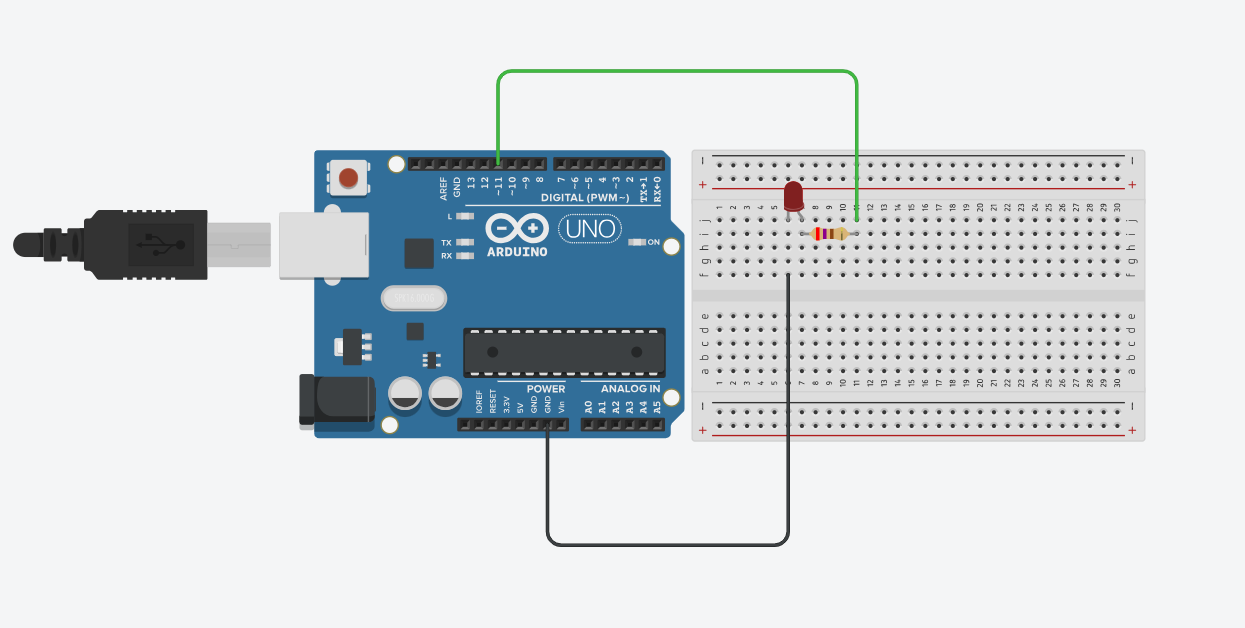
\includegraphics[width=0.7\textwidth]{led.png}
    \caption{Conectarea unui led la arduino}
    \label{fig:arduino}
\end{figure}
Plecând de la configurația atașată mută pinul de la anod pe 8 și fă-l să se aprindă și stingă la un anumit interval de timp

\begin{lstlisting}[language=C++]
// Definirea pinului la care este conectat LED-ul
const int ledPin = ?; // alege pinul corespunzator 

void setup() {
  pinMode(ledPin, ?); // Seteaza pinul LED-ului ca iesire
}

void loop() {
  digitalWrite(ledPin, ?); // Aprinde LED-ul
  delay(?);                // Asteapta 1 secundă (1000 milisecunde)

  digitalWrite(ledPin, ?);  // Stinge LED-ul
  delay(?);                // Asteapta 1 secunda
}


\end{lstlisting}
\newpage
\vspace*{1cm}
\item Numără de la 0 la 10, incrementând la fiecare secundă, și afișează valorile în monitorul serial.
\end{itemize}

\begin{lstlisting}
    // Variabila pentru a stoca valoarea curenta
int counter = 0;

void setup() {
  Serial.begin(?); // Intializeaza comunicarea seriala la o viteza de  baud
}

void loop() {
  if (counter <= ?) {            // Verifica daca numaratoarea este pana la 10
    Serial.print("Numar: ");      // Afiseaza textul
    Serial.println(?);      // Afiseaza valoarea curenta a numaratorii
    counter++;                    // Incrementeaza valoarea cu 1
    delay(?);                  // Asteapta 1 secunda
  } else {
    // Opreste numaratoarea după 10
    Serial.println("Numaratoarea s-a terminat!");
    while (?); // Blocheaza executia intr-o bucla infinita
  }
}

\end{lstlisting}



\section{ESP32-CAM}
Modulul ESP32-CAM este utilizat pentru capturarea imaginilor feței utilizatorului. Acesta transmite imaginile către un script Python pentru procesare.

\begin{figure}[H]
    \centering
    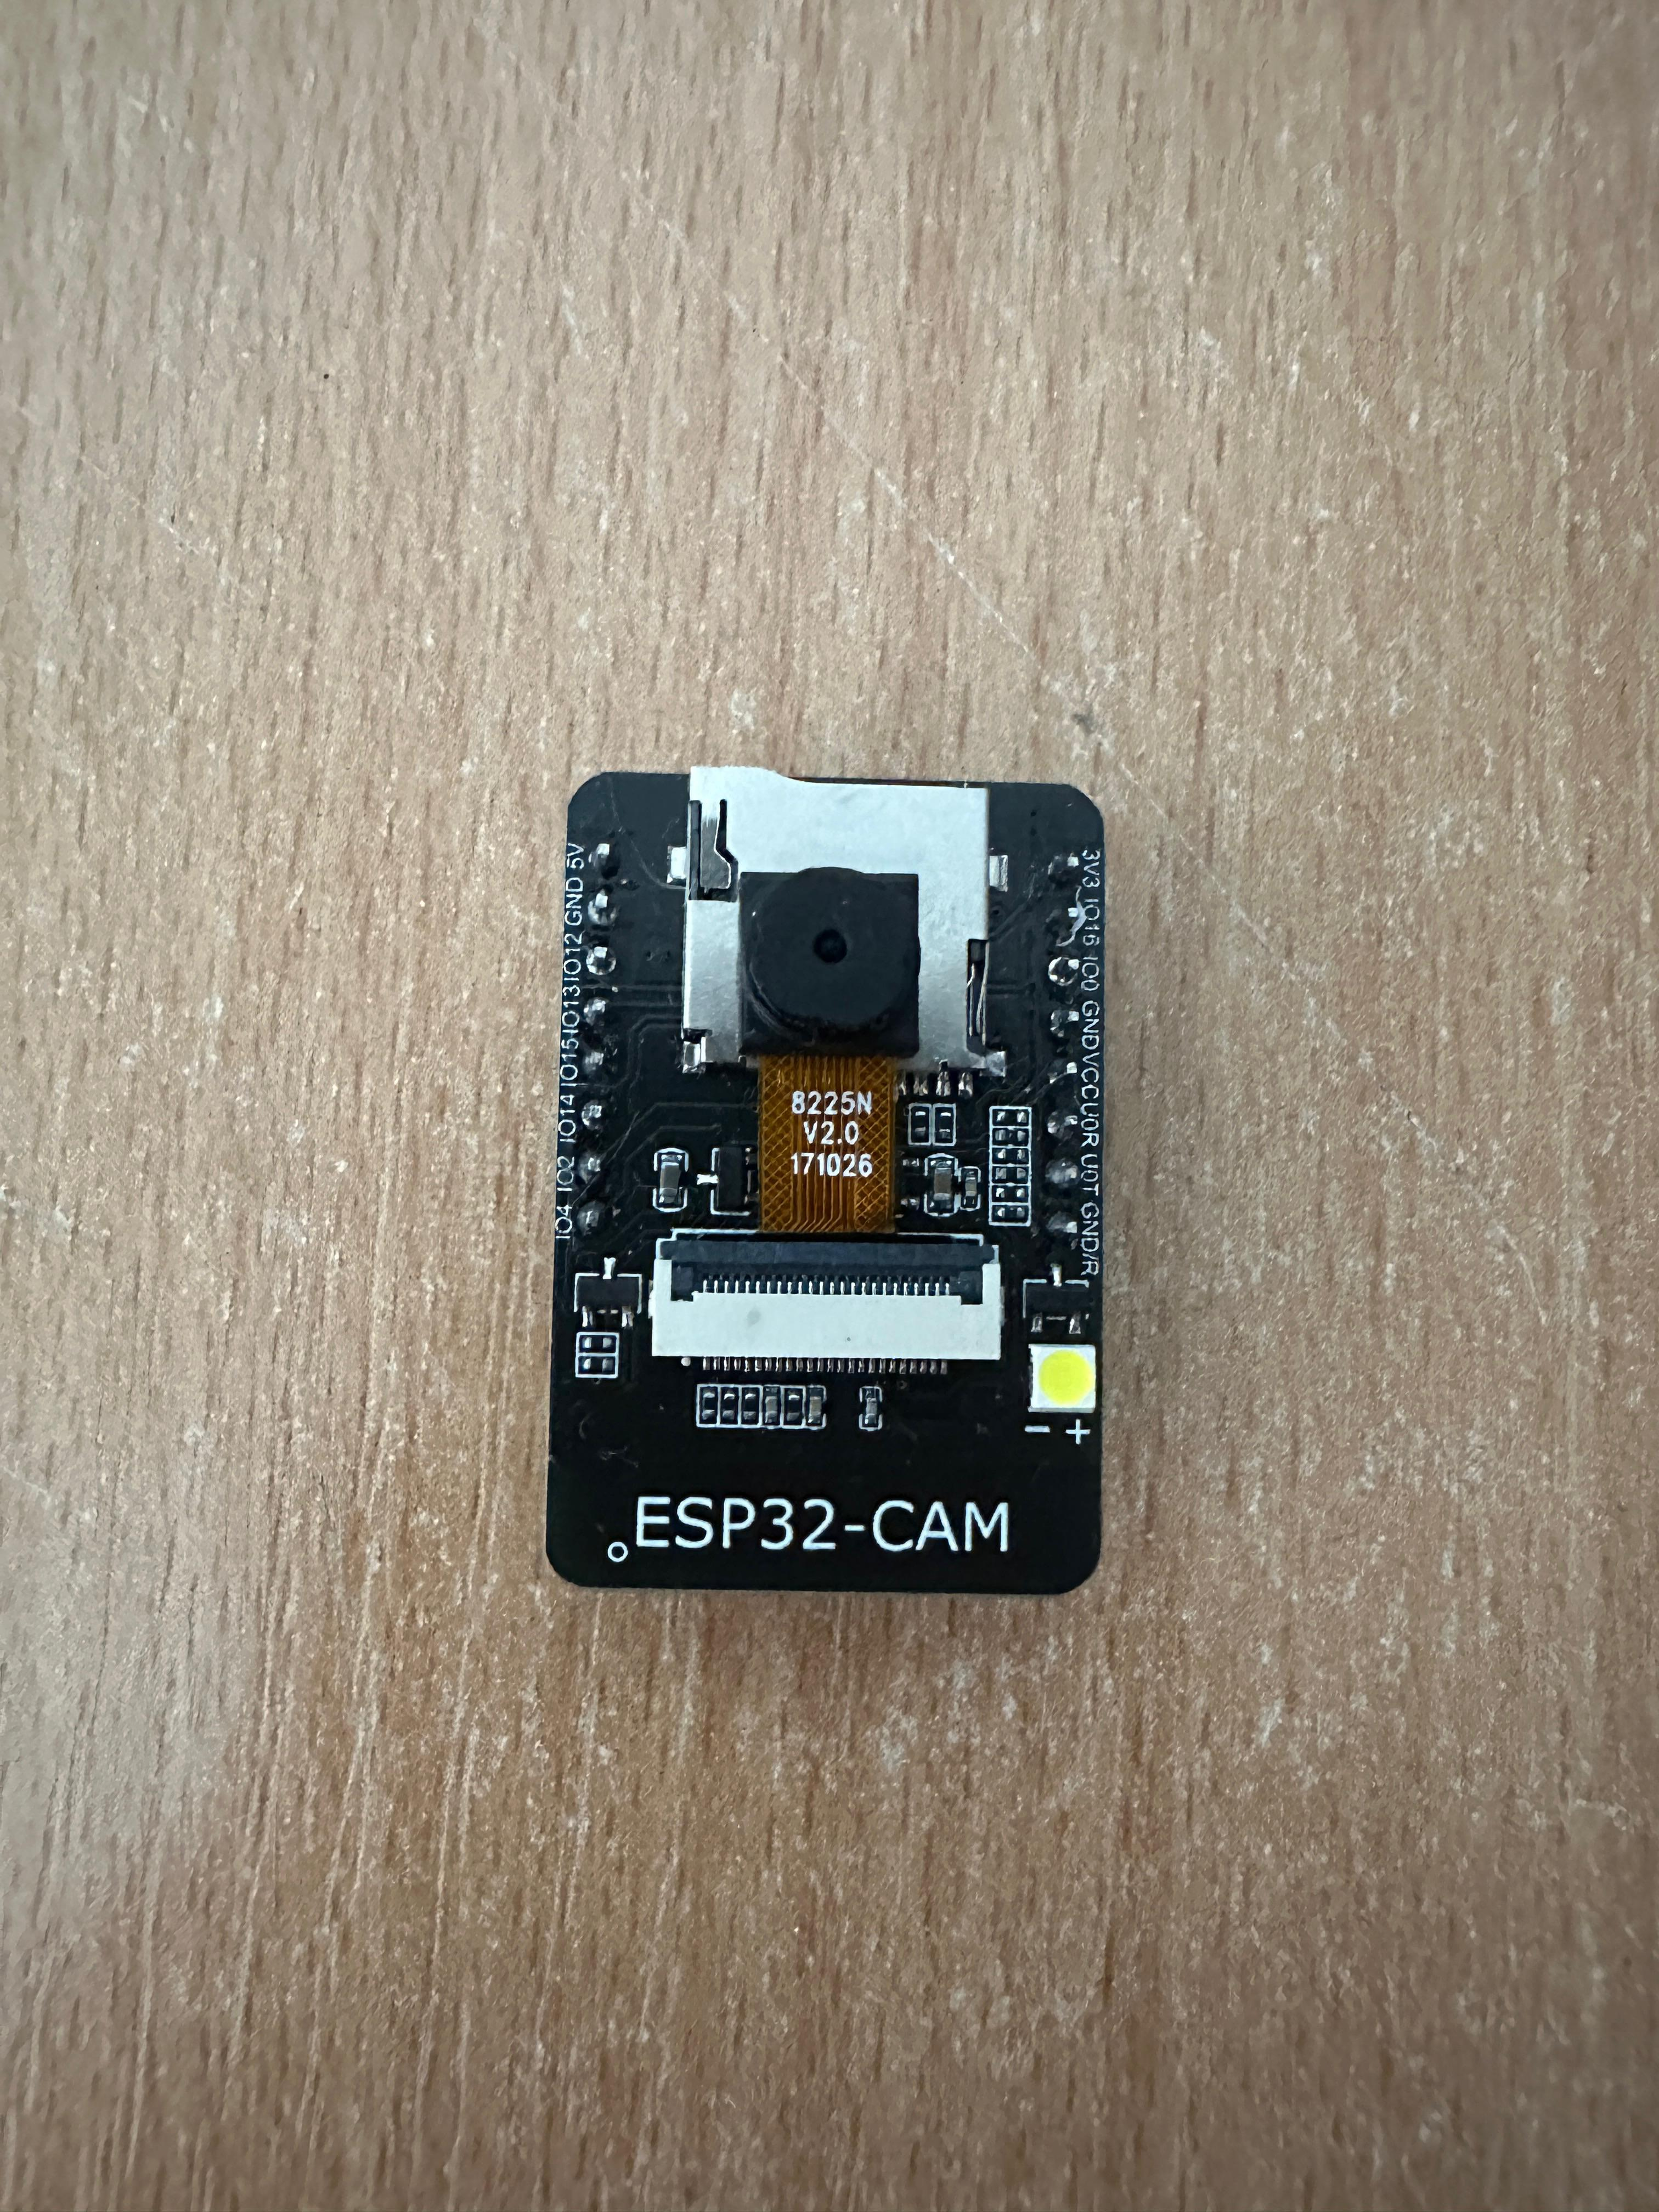
\includegraphics[width=0.6\textwidth]{esp32_cam.jpg}
    \caption{Modul ESP32-CAM}
    \label{fig:esp32_cam}
\end{figure}
\subsection*{Aplicații pentru studenți}
\begin{enumerate}
    \item Conectează ESP32-CAM la Arduino UNO conform schemei date.
    \begin{figure}[H]
    \centering
    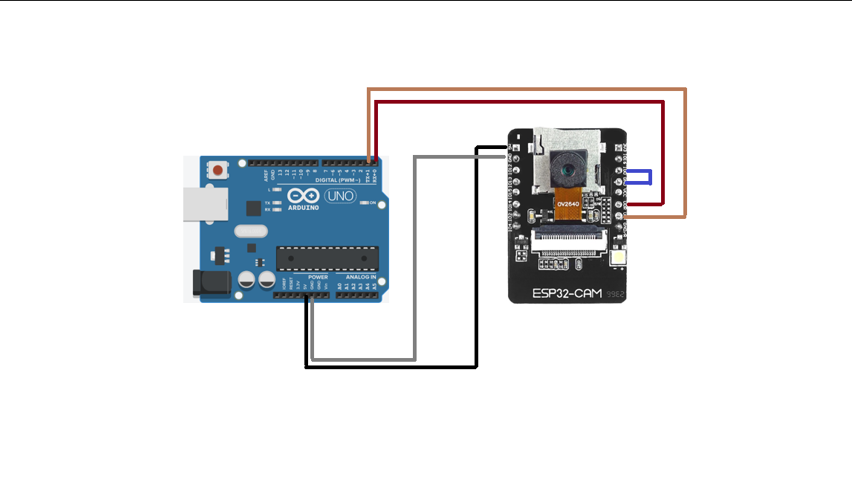
\includegraphics[width=0.8\textwidth]{schema_esp.png}
    \caption{Legătura între Arduino și ESP32-CAM}
    \label{fig:esp32_cam}
\end{figure}
\newpage
\vspace*{1cm}
După ce te asiguri că ai încărcat exemplul corespunzător pentru ESP32 Wrover Module, configurarea modulului trebuie realizată conform pașilor descriși în figura de mai jos:

\begin{figure}[H]
    \centering
    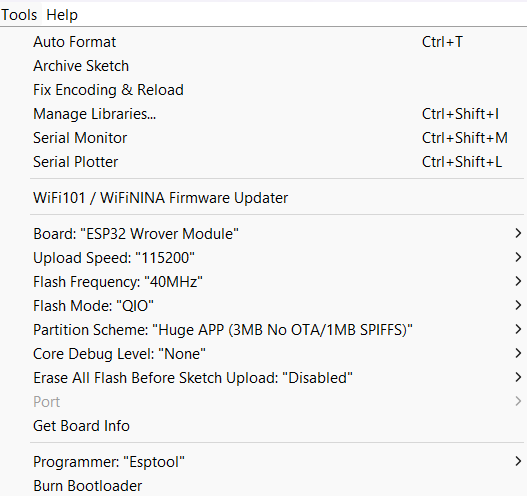
\includegraphics[width=0.8\textwidth]{cameraWebServer_tools.png}
    \caption{Confirmare ESP32 Wrover Module}
    \label{fig:esp}
\end{figure}

Accesarea fluxului video al camerei prin adresa IP:
\begin{itemize}
    \item Asigură-te că ai introdus corect credențialele WiFi (ssid și password) în codul ESP32-CAM. Compilează și încarcă codul pe ESP32-CAM.
\begin{lstlisting}
    #include "esp_camera.h"
#include <WiFi.h>

//
// WARNING!!! PSRAM IC required for UXGA resolution and high JPEG quality
//            Ensure ESP32 Wrover Module or other board with PSRAM is selected
\end{lstlisting}
\vspace*{1cm}
\begin{lstlisting}
//            Partial images will be transmitted if image exceeds buffer size
//
//            You must select partition scheme from the board menu that has at least 3MB APP space.
//            Face Recognition is DISABLED for ESP32 and ESP32-S2, because it takes up from 15 
//            seconds to process single frame. Face Detection is ENABLED if PSRAM is enabled as well

// ===================
// Select camera model
// ===================
//#define CAMERA_MODEL_WROVER_KIT // Has PSRAM
//#define CAMERA_MODEL_ESP_EYE // Has PSRAM
//#define CAMERA_MODEL_ESP32S3_EYE // Has PSRAM
//#define CAMERA_MODEL_M5STACK_PSRAM // Has PSRAM
//#define CAMERA_MODEL_M5STACK_V2_PSRAM // M5Camera version B Has PSRAM
//#define CAMERA_MODEL_M5STACK_WIDE // Has PSRAM
//#define CAMERA_MODEL_M5STACK_ESP32CAM // No PSRAM
//#define CAMERA_MODEL_M5STACK_UNITCAM // No PSRAM
#define CAMERA_MODEL_AI_THINKER // Has PSRAM
//#define CAMERA_MODEL_TTGO_T_JOURNAL // No PSRAM
// ** Espressif Internal Boards **
//#define CAMERA_MODEL_ESP32_CAM_BOARD
//#define CAMERA_MODEL_ESP32S2_CAM_BOARD
//#define CAMERA_MODEL_ESP32S3_CAM_LCD

#include "camera_pins.h"

// ===========================
// Enter your WiFi credentials
// =====  ======================
const char* ssid = "************"; //Configureaza reteaua de internet
const char* password = "********";
\end{lstlisting}
\vspace*{1cm}
\begin{lstlisting}
void startCameraServer();

void setup() {
  Serial.begin(115200);
  Serial.setDebugOutput(true);
  Serial.println();

  camera_config_t config;
  config.ledc_channel = LEDC_CHANNEL_0;
  config.ledc_timer = LEDC_TIMER_0;
  config.pin_d0 = Y2_GPIO_NUM;
  config.pin_d1 = Y3_GPIO_NUM;
  config.pin_d2 = Y4_GPIO_NUM;
  config.pin_d3 = Y5_GPIO_NUM;
  config.pin_d4 = Y6_GPIO_NUM;
  config.pin_d5 = Y7_GPIO_NUM;
  config.pin_d6 = Y8_GPIO_NUM;
  config.pin_d7 = Y9_GPIO_NUM;
  config.pin_xclk = XCLK_GPIO_NUM;
  config.pin_pclk = PCLK_GPIO_NUM;
  config.pin_vsync = VSYNC_GPIO_NUM;
  config.pin_href = HREF_GPIO_NUM;
  config.pin_sscb_sda = SIOD_GPIO_NUM;
  config.pin_sscb_scl = SIOC_GPIO_NUM;
  config.pin_pwdn = PWDN_GPIO_NUM;
  config.pin_reset = RESET_GPIO_NUM;
  config.xclk_freq_hz = 20000000;
  config.frame_size = FRAMESIZE_UXGA;
  config.pixel_format = PIXFORMAT_JPEG; // for streaming
  //config.pixel_format = PIXFORMAT_RGB565; // for face detection/recognition
  config.grab_mode = CAMERA_GRAB_WHEN_EMPTY;
  config.fb_location = CAMERA_FB_IN_PSRAM;
  config.jpeg_quality = 12;
  config.fb_count = 1;
  
  // if PSRAM IC present, init with UXGA resolution and higher JPEG quality
  //                      for larger pre-allocated frame buffer.
  \end{lstlisting}
  \vspace*{1cm}
  \begin{lstlisting}
  if(config.pixel_format == PIXFORMAT_JPEG){
    if(psramFound()){
      config.jpeg_quality = 10;
      config.fb_count = 2;
      config.grab_mode = CAMERA_GRAB_LATEST;
    } else {
      // Limit the frame size when PSRAM is not available
      config.frame_size = FRAMESIZE_SVGA;
      config.fb_location = CAMERA_FB_IN_DRAM;
    }
  } else {
    // Best option for face detection/recognition
    config.frame_size = FRAMESIZE_240X240;
#if CONFIG_IDF_TARGET_ESP32S3
    config.fb_count = 2;
#endif
  }

#if defined(CAMERA_MODEL_ESP_EYE)
  pinMode(13, INPUT_PULLUP);
  pinMode(14, INPUT_PULLUP);
#endif

  // camera init
  esp_err_t err = esp_camera_init(&config);
  if (err != ESP_OK) {
    Serial.printf("Camera init failed with error 0x%x", err);
    return;
  }

  sensor_t * s = esp_camera_sensor_get();
  // initial sensors are flipped vertically and colors are a bit saturated
  if (s->id.PID == OV3660_PID) {
    s->set_vflip(s, 1); // flip it back
    s->set_brightness(s, 1); // up the brightness just a bit
    s->set_saturation(s, -2); // lower the saturation
  }
  \end{lstlisting}
  \vspace*{1cm}
  \begin{lstlisting}
  // drop down frame size for higher initial frame rate
  if(config.pixel_format == PIXFORMAT_JPEG){
    s->set_framesize(s, FRAMESIZE_QVGA);
  }

#if defined(CAMERA_MODEL_M5STACK_WIDE) || defined(CAMERA_MODEL_M5STACK_ESP32CAM)
  s->set_vflip(s, 1);
  s->set_hmirror(s, 1);
#endif

#if defined(CAMERA_MODEL_ESP32S3_EYE)
  s->set_vflip(s, 1);
#endif

  WiFi.begin(ssid, password);
  WiFi.setSleep(false);

  while (WiFi.status() != WL_CONNECTED) {
    delay(500);
    Serial.print(".");
  }
  Serial.println("");
  Serial.println("WiFi connected");

  startCameraServer();

  Serial.print("Camera Ready! Use 'http://");
  Serial.print(WiFi.localIP());
  Serial.println("' to connect");
}

void loop() {
  // Do nothing. Everything is done in another task by the web server
  delay(10000);
}
\end{lstlisting}

    \item Pas 2: Deschide Monitorul Serial din Arduino IDE (setat la baud rate 115200). Așteaptă până vezi mesajul:
    \begin{verbatim}
        Camera Ready! Use 'http://<adresa IP>' to connect

    \end{verbatim}
    Notează adresa IP afișată.
    \item Introdu adresa IP în browserul unui dispozitiv conectat la aceeași rețea WiFi. Vei vedea interfața web a serverului camerei.
    \item  Explorează setările oferite în interfață 
\end{itemize}

    \item Modificarea rezoluției imaginii din interfața web
    \begin{itemize}
        \item  Repetă pașii din Exercițiul 1 pentru a accesa fluxul video al camerei din browser
        \item În interfața web, localizează secțiunea "Resolution" (sau o secțiune similară)
        \item Pas 3: Schimbă rezoluția imaginii, de exemplu
        \begin{verbatim}
            De la QVGA (320x240) la SVGA (800x600)
        \end{verbatim}
        \item Observă schimbarea calității imaginii în fluxul video
        
        \textbf{Rezultatul așteptat: }Rezoluția fluxului video se va schimba imediat, iar performanța (viteză sau claritate) va varia în funcție de rezoluție
    \end{itemize}
\end{enumerate}
\vspace*{1cm}




\section{Motor servo MG996R}
Motorul servo este responsabil pentru deschiderea mecanismului fizic al ușii sau sertarului. Este controlat prin semnale PWM generate de Arduino.

\begin{figure}[H]
    \centering
    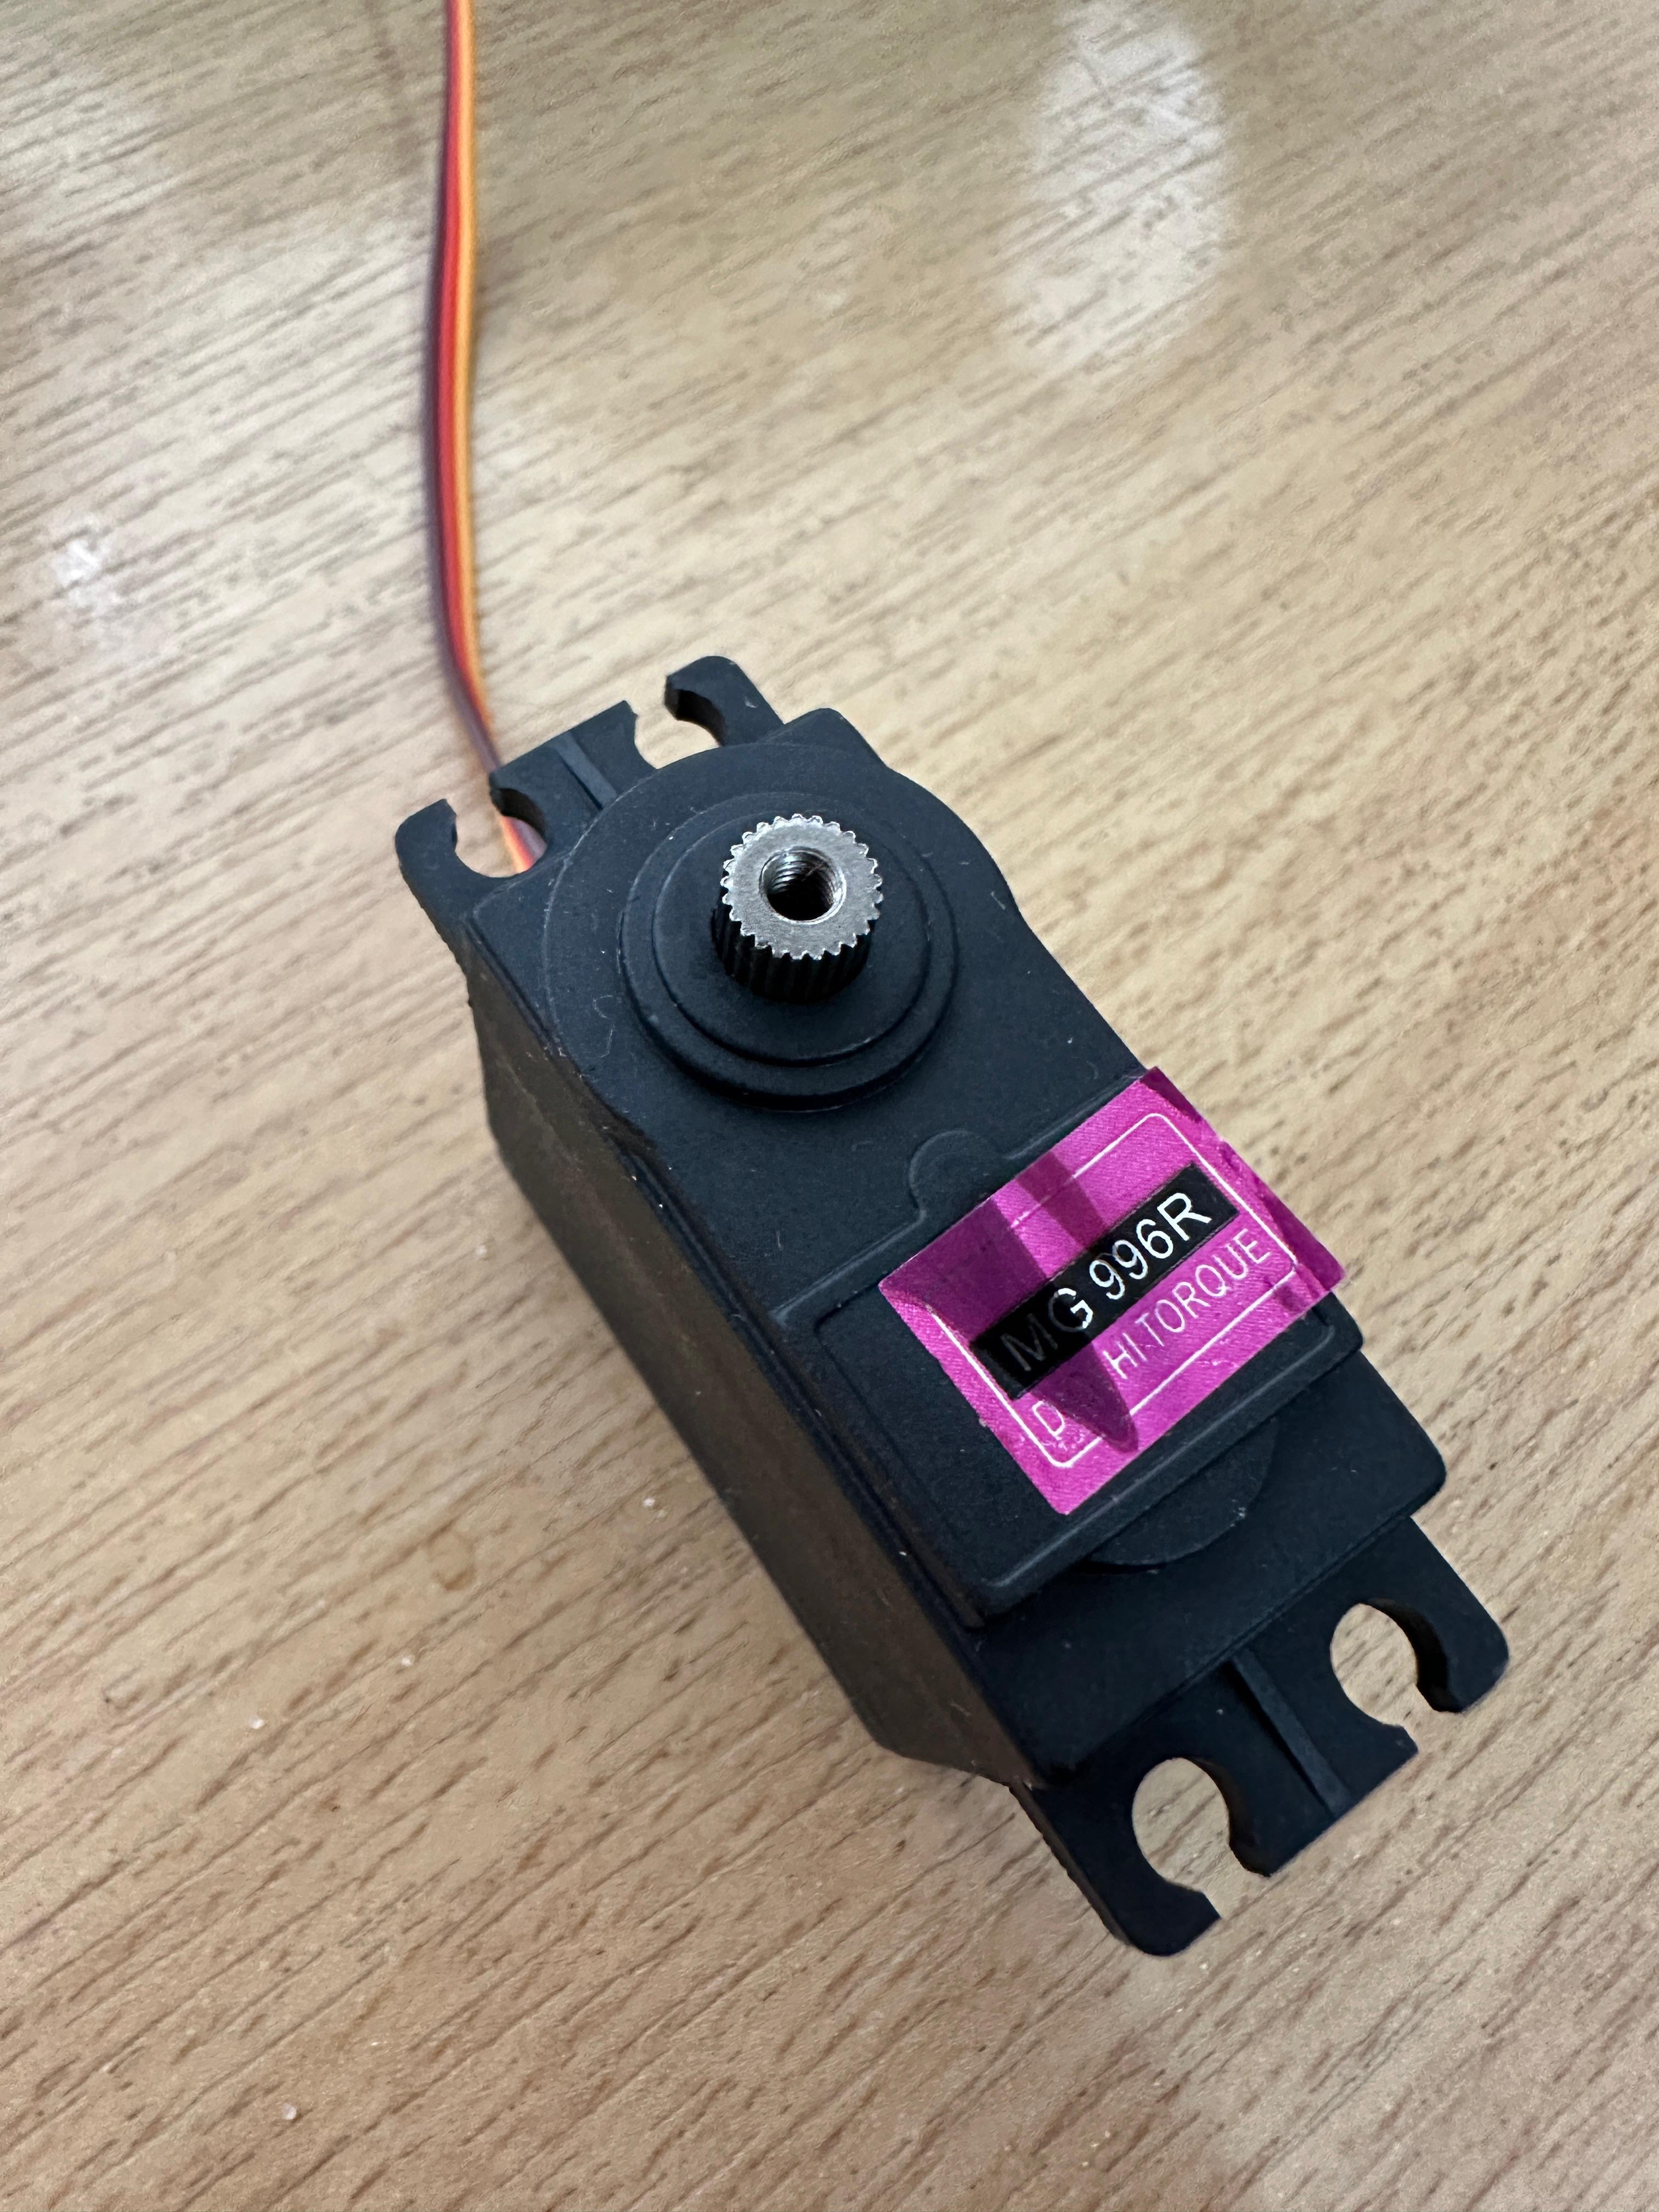
\includegraphics[width=0.6\textwidth]{servo_motor.jpg}
    \caption{Motor servo MG996R}
    \label{fig:servo_motor}
\end{figure}

\begin{figure}[H]
    \centering
    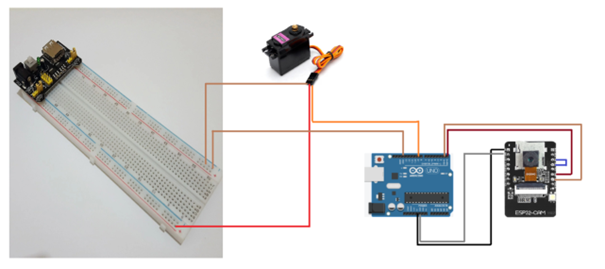
\includegraphics[width=0.9\textwidth]{motorEX.png}
    \caption{Conectare servo MG996R la arduino}
    \label{fig:servo_motor}
\end{figure}
\newpage
\vspace*{1cm}
\subsection*{Aplicații pentru studenți}
\begin{itemize}
    \item  Mișcă servo-ul între 0° și 180° cu pauză
\begin{lstlisting}
    #include <Servo.h>

Servo myServo; // Cream un obiect Servo pentru a controla motorul
const int servoPin = ?; // Pinul la care este conectat servo-ul în configuratie

void setup() {
  myServo.attach(servoPin); // Atasam pinul servo-ului
}

void loop() {
  // Misca servo-ul de la 0° la 180°
  for (int pos = ?; pos <= ?; pos++) {
    myServo.write(pos); // Seteaza pozitia servo-ului
    delay(15); // Pauza pentru a permite motorului sa se miste
  }
    \end{lstlisting}
    \vspace*{1cm}
\begin{lstlisting}
  
  delay(?); // Pauza 1 secunda
  
  // Misca servo-ul inapoi de la 180° la 0°
  for (int pos = ?; pos >= 0; pos--) {
    myServo.write(pos);
    delay(15);
  }  
  delay(1000); // Pauza 1 secunda
}

\end{lstlisting}
    \item Mișcă servo-ul în funcție de mesajul primit de la LCD.
\end{itemize}
\begin{lstlisting}
#include <Servo.h>
#include <Wire.h>
\end{lstlisting}
\vspace*{1cm}
\begin{lstlisting}
#include <LiquidCrystal_I2C.h>

// Obiecte pentru servomotor și LCD
Servo myservo;
LiquidCrystal_I2C lcd(0x27, 16, 2); // Adresa LCD-ului I2C

// Variabile globale
bool isAccessGranted = false; // Flag pentru acces

void setup() {
 // LIPSA: Initializare conexiune seriala
 // LIPSA: Ataseaza pinul de control al servomotorului
 // LIPSA: Seteaza pozitia initiala a servomotorului

  lcd.init();
  lcd.backlight();
  lcd.clear();
 // LIPSA: Mesajul initial pe LCD
  delay(2000);
  lcd.clear();
}

void loop() {
  if (Serial.available() > 0) {
 // LIPSA: Citire mesaj serial
    if (message == "PERMIS") {
      isAccessGranted = true;
      lcd.clear();
      lcd.print("Acces permis");
     // LIPSA: Poziția pentru acces permis
    } else if (message == "RESPINS") {
      isAccessGranted = false;
      lcd.clear();
      lcd.print("Acces respins");
 // LIPSA: Revine la pozitia initiala
    }
  }
}


\end{lstlisting}


\newpage
\vspace*{1cm}
\section{LCD 16x2 cu I2C}
LCD-ul afișează mesaje pentru utilizator, precum „Acces permis” sau „Acces permis”. Este conectat la Arduino prin interfața I2C, reducând numărul de pini necesari.

\begin{figure}[H]
    \centering
    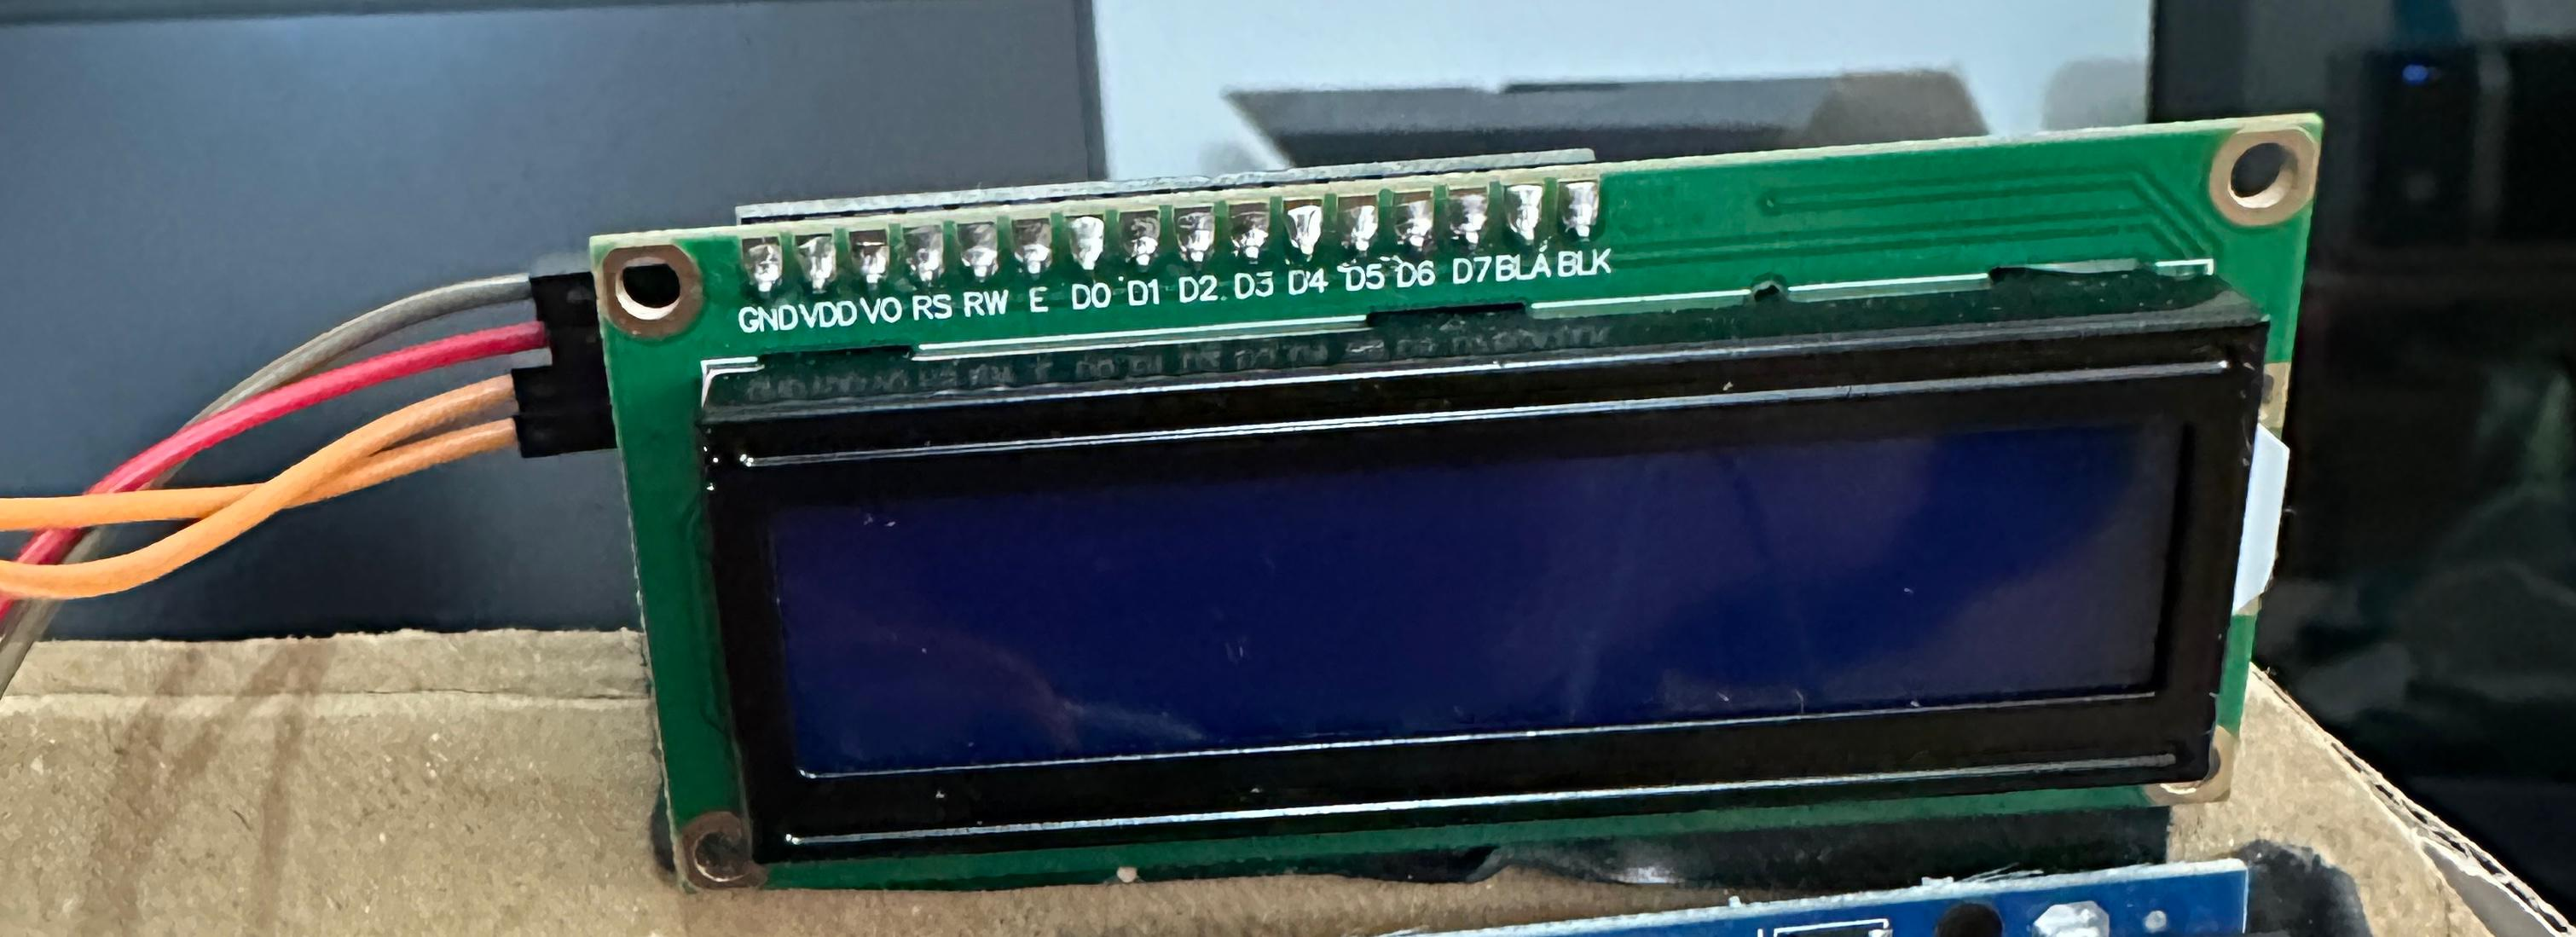
\includegraphics[width=0.6\textwidth]{lcd_i2c.jpg}
    \caption{LCD 16x2 cu I2C}
    \label{fig:lcd_i2c}
\end{figure}


\begin{figure}[H]
    \centering
    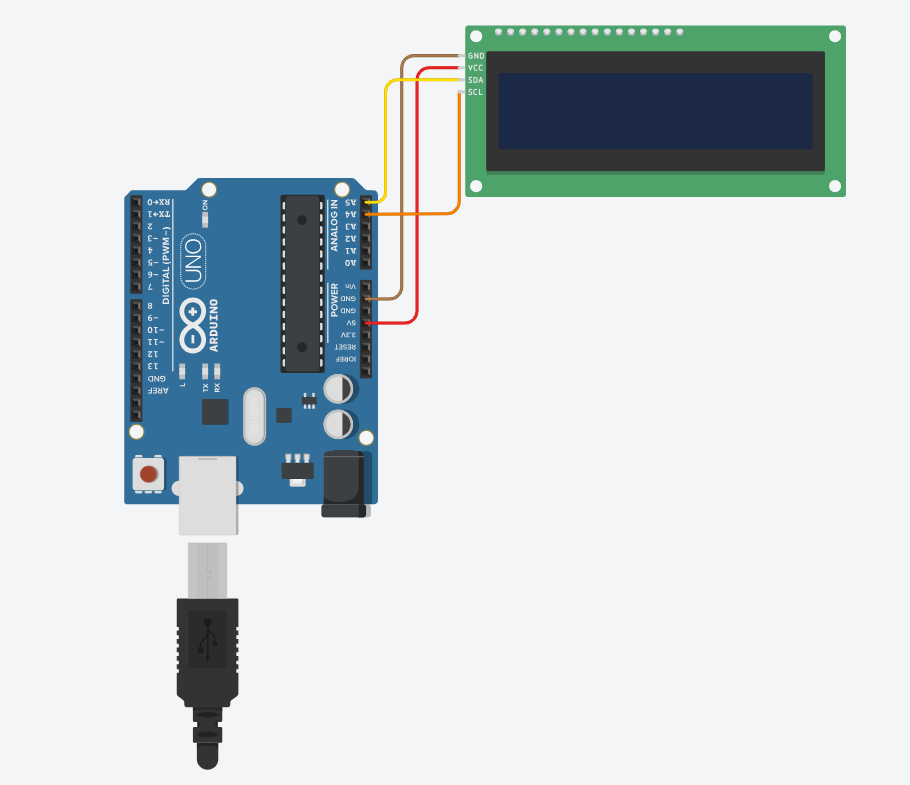
\includegraphics[width=0.5\linewidth]{montaj-lcd+arduino.png}
    \caption{Configurație LCD 16x2 cu I2C}
    \label{fig:enter-label}
\end{figure}

\subsection*{Aplicații pentru studenți}
\begin{itemize}
    \item Afișarea unui mesaj static, precum "Bun venit!".
    \begin{lstlisting}
#include <Wire.h>
#include <LiquidCrystal_I2C.h>

// Initializare LCD cu adresa I2C
LiquidCrystal_I2C lcd(0x27, 16, 2); // Adresa poate fi diferita (verifica in functie de modulul tau)
\end{lstlisting}
\newpage
\vspace*{1cm}
\begin{lstlisting}
void setup() {
  lcd.init();        // Initializare LCD
  lcd.backlight();   // Activeaza iluminarea de fundal
  // LINIA LIPSA: Curata ecranul

  // LINIE LIPSA: Afiseaza mesajul
}

void loop() {
  // Bucla principala nu face nimic
}

    \end{lstlisting}
    \item Afișarea accesului permis sau respins. Acest exercițiu integrează LCD-ul pentru a afișa „Acces permis” sau „Acces respins” pe baza mesajelor primite
    \begin{lstlisting}
#include <Servo.h>
#include <Wire.h>
#include <LiquidCrystal_I2C.h>

// Obiecte pentru servomotor și LCD
Servo myservo;
LiquidCrystal_I2C lcd(0x27, 16, 2); // Adresa LCD-ului I2C

// Variabile globale
bool isAccessGranted = false; // Flag pentru acces

void setup() {
  Serial.begin(?);     // Initializare conexiune seriala
  myservo.attach(9);        // Pinul de semnal pentru servomotor
  myservo.write(?);         // Pozitia initiala a servomotorului

// LINIE LIPSA:Initializare LCD
  lcd.backlight();          // Activeaza iluminarea de fundal
\end{lstlisting}
\newpage
\vspace*{1cm}
\begin{lstlisting}
  lcd.clear();
  ; // LINIE LIPSA: Afiseaza mesajul "Asteptare..."
}

void loop() {
  if (Serial.available() > 0) {
    String message = Serial.readStringUntil('\n'); // Citire mesaj

    if (message == "PERMIS") {
      isAccessGranted = true;
      lcd.clear();
      // LINIE LIPSA: Afiseaza mesajul "Acces permis"
      Serial.println("Acces permis");
    } else if (message == "RESPINS") {
      isAccessGranted = false;
      lcd.clear();
      ; // LINIE LIPSA: Afiseaza mesajul "Acces respins"
      Serial.println("Acces respins");
    } else {
      lcd.clear();
      ; // LINIE LIPSA: Afiseaza mesajul "Mesaj necunoscut"
      Serial.println("Mesaj necunoscut primit");
    }
  }

  // Miscare servomotor daca accesul este permis
  if (isAccessGranted) {
    myservo.write(90); // Deschide servomotorul
    delay(?);       // LINIE LIPSA: Asteapta 2 secunde
    myservo.write(0);  // inchide servomotorul
    isAccessGranted = false; // Reseteaza flag-ul
  }
}

    \end{lstlisting}
\end{itemize}


\newpage
\vspace*{1cm}
\section{LED-uri}
LED-urile indică starea accesului: verde pentru acces autorizat, roșu pentru acces respins.

\begin{figure}[H]
    \centering
    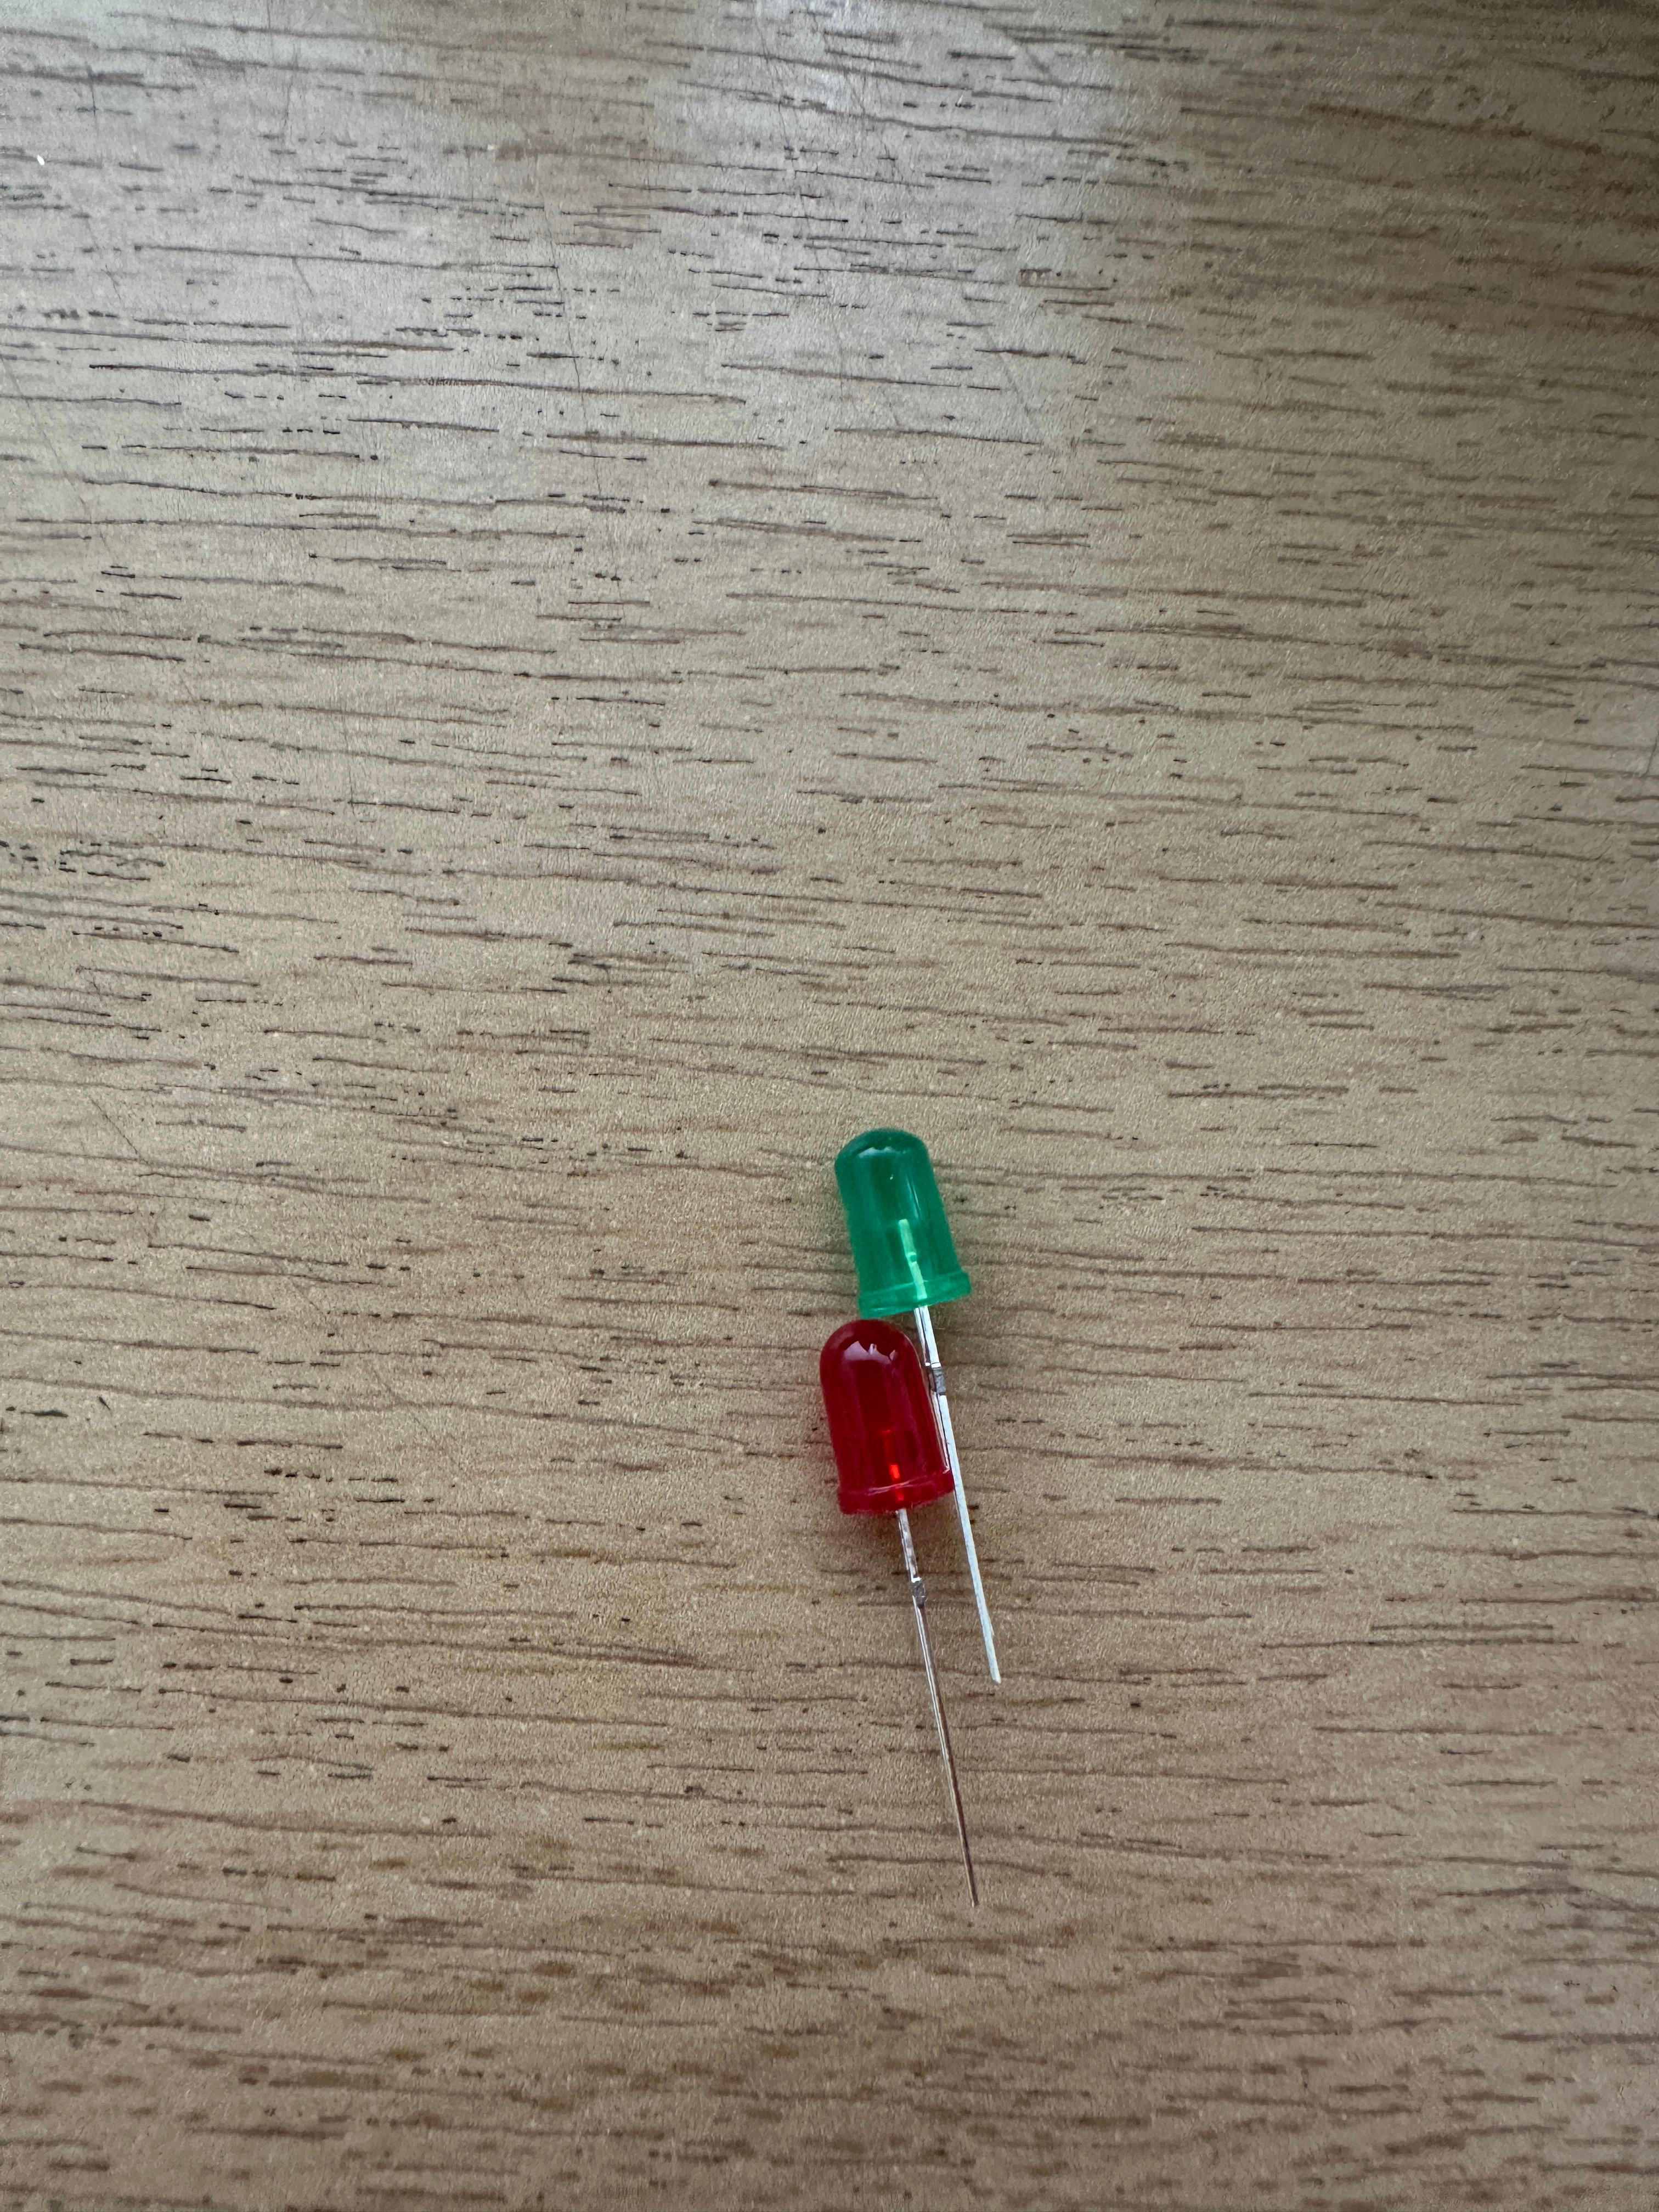
\includegraphics[width=0.4\textwidth]{leds.jpg}
    \caption{LED-uri utilizate în proiect}
    \label{fig:leds}
\end{figure}

\begin{figure}[H]
    \centering
    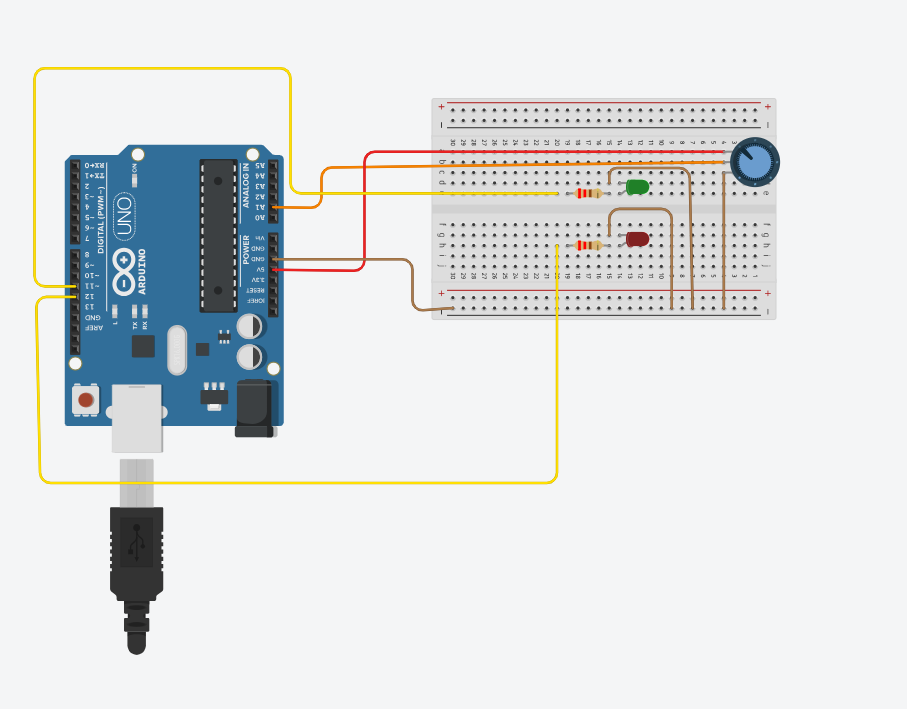
\includegraphics[width=0.5\linewidth]{led+pot.png}
    \caption{Configurare led-uri și potențiometru}
    \label{fig:configleds}
\end{figure}
\newpage
\vspace*{1cm}
\subsection*{Aplicații pentru studenți}
\begin{itemize}
    \item Crearea unui semnal intermitent (blink) pentru un LED.
    \begin{lstlisting}
  void setup() {
  pinMode(ledGreen, OUTPUT); // Configureaza LED-ul verde ca iesire
}

void loop() {
    // LIPSA: Aprinde LED-ul verde
  delay(500);                   // Asteapta 500ms
    // LIPSA: Stinge LED-ul verde
  delay(500);                   // Asteapta 500ms
}

    \end{lstlisting}
    \item Aprinderea LED-urilor în funcție de accesul permis sau respins.
    \begin{lstlisting}
  void setup() {
  pinMode(ledGreen, OUTPUT); // Configureaza LED-ul verde ca iesire
 // LIPSA: Configureaza LED-ul rosu ca iesire
  Serial.begin(115200);      // Porneste comunicatia seriala
}

void loop() {
  if (Serial.available() > 0) {
    String message = Serial.readStringUntil('\n'); // Citeste mesajul trimis prin serial

    if (message == "PERMIS") {
     // LIPSA: Aprinde LED-ul verde
     // LIPSA: Stinge LED-ul rosu
      Serial.println("Acces permis: LED verde aprins");
    } else if (message == "RESPINS") {
       // LIPSA: Stinge LED-ul verde
       // LIPSA: Aprinde LED-ul rosu
      Serial.println("Acces respins: LED rosu aprins");
      \end{lstlisting}
      \newpage
      \vspace*{1cm}
      \begin{lstlisting}
    } else {
      digitalWrite(ledGreen, LOW); // Stinge ambele LED-uri
      digitalWrite(ledRed, LOW);
      Serial.println("Mesaj necunoscut: Ambele LED-uri stinse");
    }
  }
}

    \end{lstlisting}
\end{itemize}



\section{Potențiometru}
Potențiometrul este utilizat pentru ajustarea contrastului LCD-ului sau a intensității LED-urilor.
Pentru o bună funționare asigură conctarea acestei componente conform \textbf{Figurii \ref{fig:configleds}}.
LCD-ul fiind cu I2C deține deja pe spate un mic potențiometru de culoare albastră care poate fi reglat ușor cu o șurubelniță mică, iar potențiometrul atașat din imagine este folosit în ajustarea intensității led-urilor din proiect.
\begin{figure}[H]
    \centering
    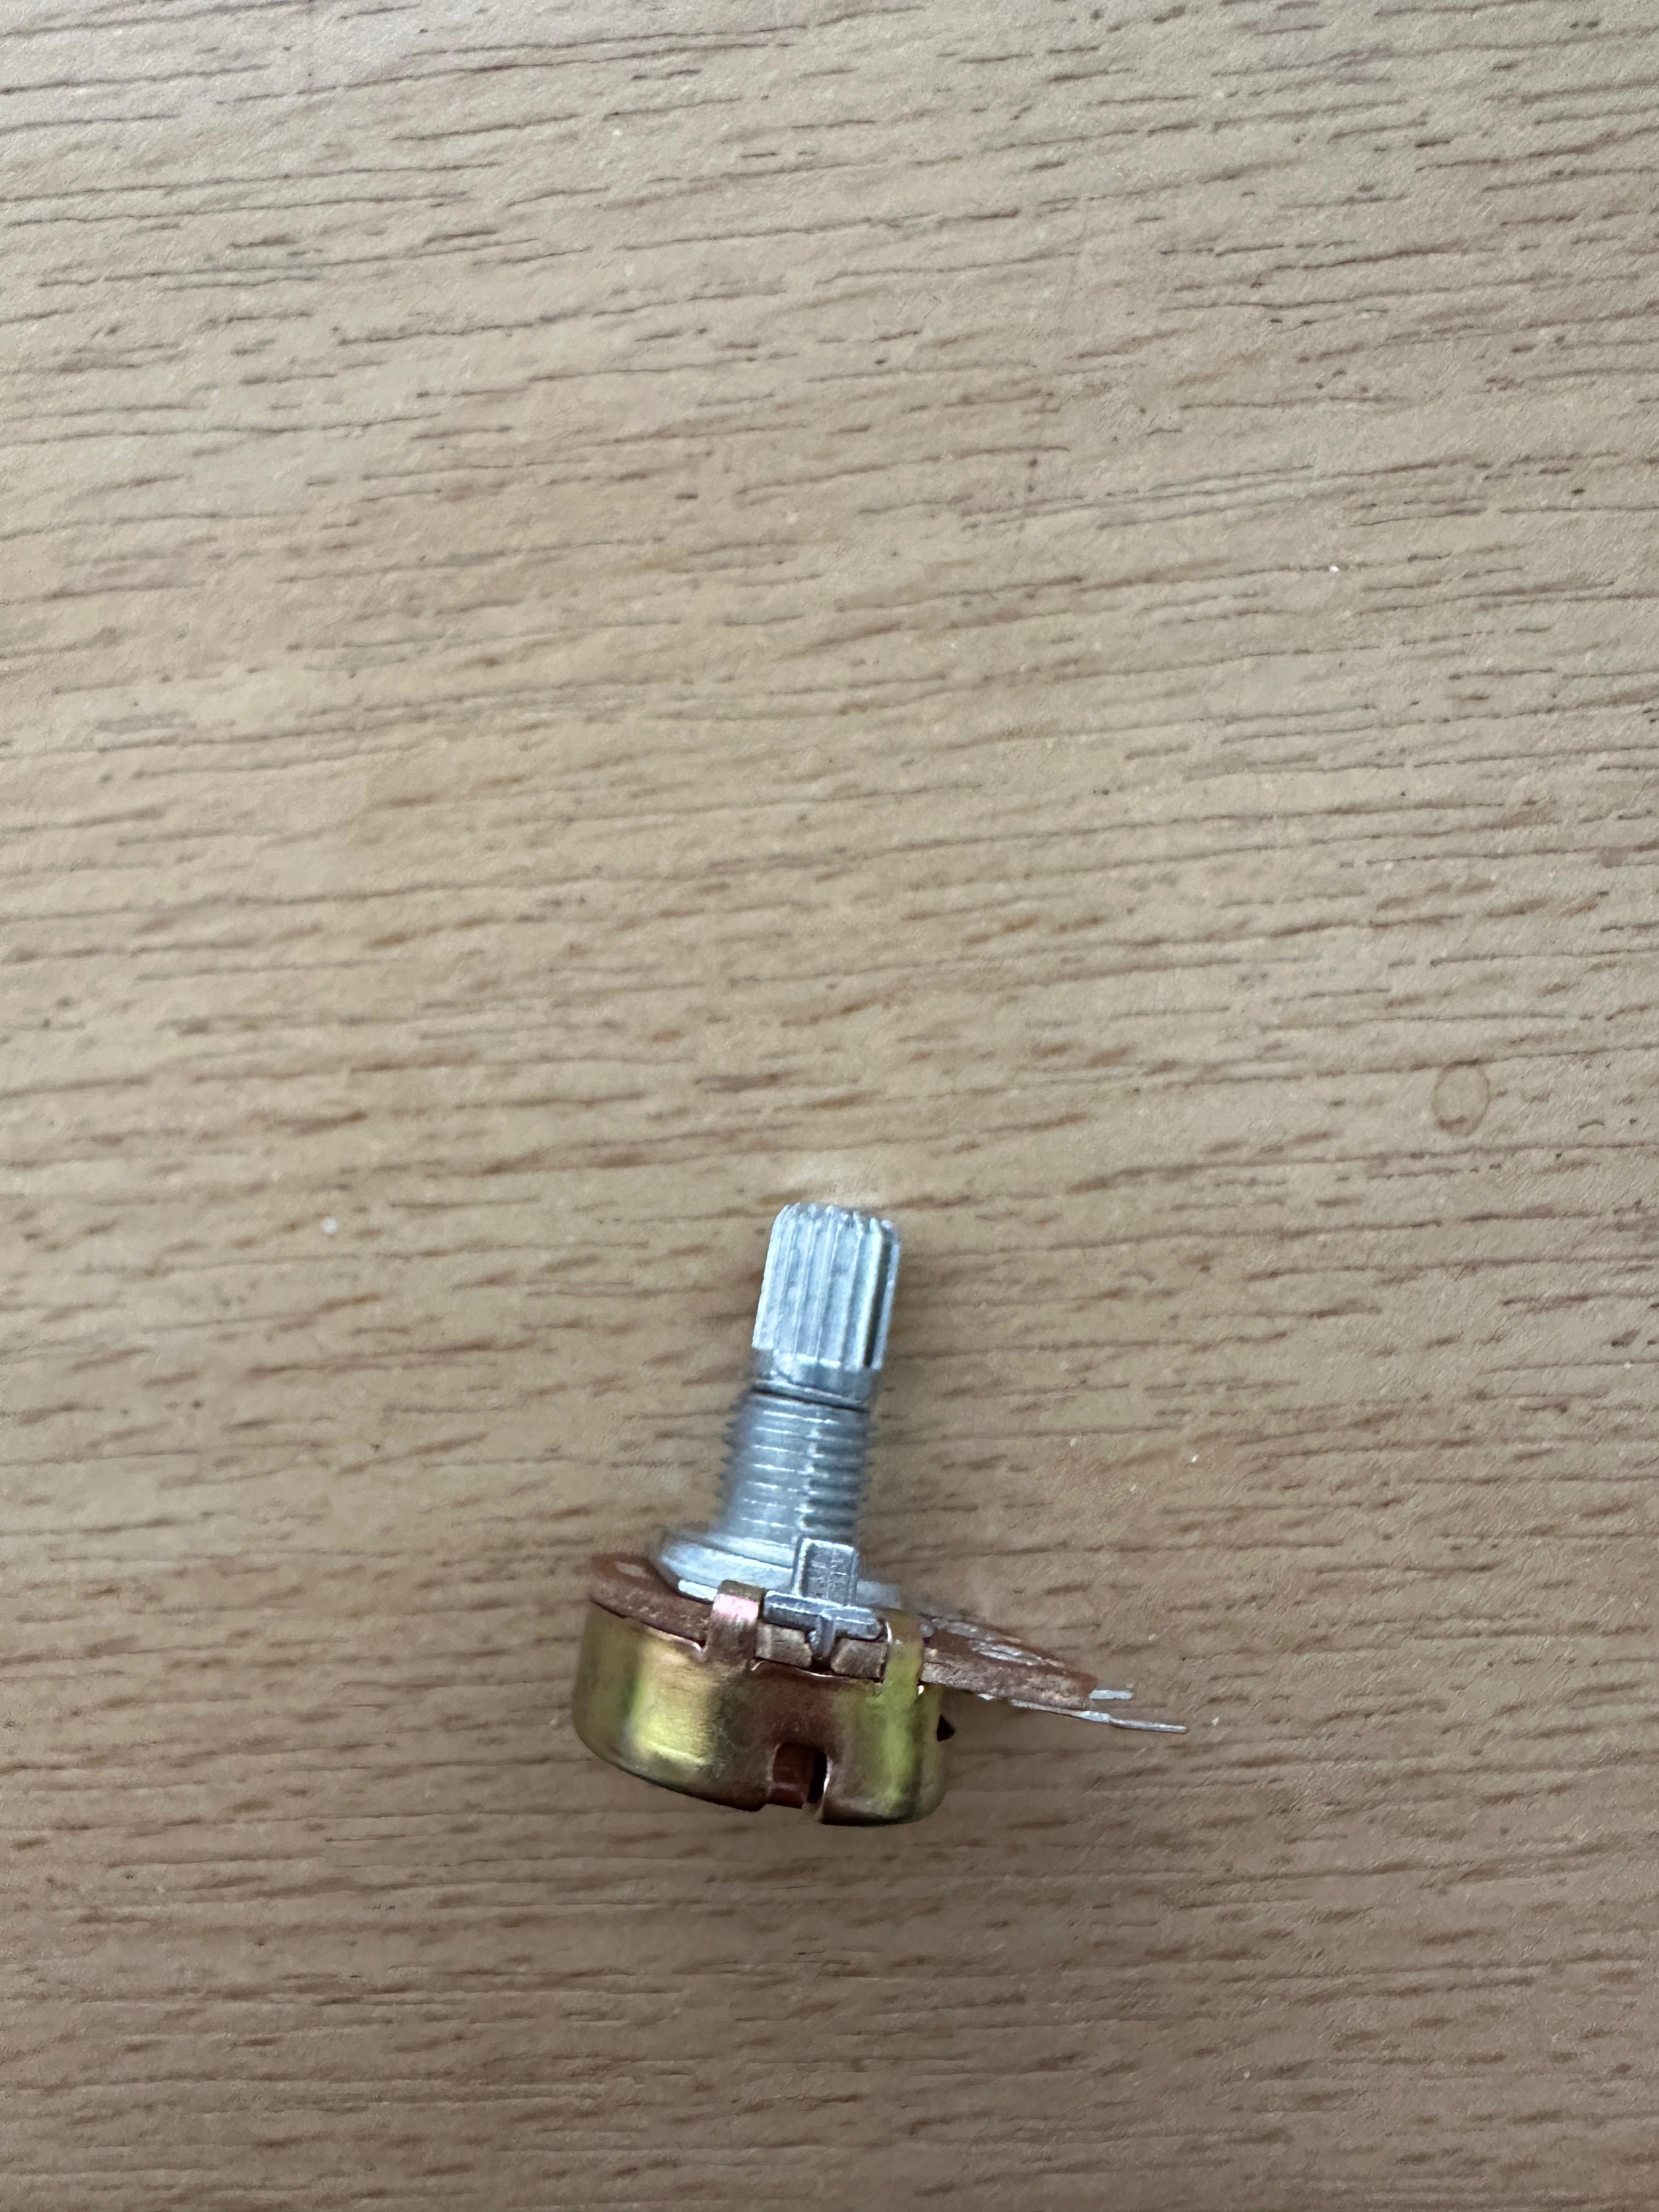
\includegraphics[width=0.5\textwidth]{potentiometru.jpg}
    \caption{Potențiometru pentru ajustare }
    \label{fig:potentiometer}
\end{figure}
\newpage
\vspace*{1cm}
\subsection*{Aplicații pentru studenți}
\begin{itemize}
    \item Reglarea luminozității unui LED prin citirea poziției potentiometrului.
    Acest exercițiu implementează funcționalitatea de a ajusta intensitatea luminii LED-urilor (verde și roșu) pe baza valorii citite de la potențiometru, așa cum se observă în codul principal al proiectului
    \begin{lstlisting}
const int potentiometerPin = ?; // Pin pentru potentiometru
const int ledGreen = 12;        // Pin pentru LED verde
const int ledRed = 11;          // Pin pentru LED rosu

void setup() {
  pinMode(ledGreen, OUTPUT);    // Configureaza LED-ul verde ca iesire
  pinMode(ledRed, OUTPUT);      // Configureaza LED-ul rosu ca iesire
  Serial.begin(115200);         // Porneste comunicatia seriala
}

void loop() {
  int potValue = analogRead(potentiometerPin); // Citeste valoarea analogica de la potentiometru
  int ledIntensity = map(potValue, 0, 1023, 0, 255); // Mapare valoare 0-1023 la 0-255

   // LIPSA: Ajusteaza intensitatea LED-ului verde
   // LIPSA: Ajusteaza intensitatea LED-ului rosu

  delay(?); // Pauza scurta pentru stabilitate 1ms
}

    \end{lstlisting}
    \newpage
    \vspace*{1cm}
    \item Citirea valorii analogice de la potentiometru și afișarea acesteia pe monitorul serial.Acest exercițiu implementează funcționalitatea de a citi valoarea analogică a potențiometrului și de a o afișa pe monitorul serial.
\end{itemize}
\begin{lstlisting}
const int potentiometerPin = A0; // Pin pentru potentiometru

void setup() {
  Serial.begin(115200); // Porneste comunicatia seriala
}

void loop() {
  int potValue = analogRead(potentiometerPin); // Citeste valoarea analogica de la potentiometru
  // LIPSA: Afiseaza textul descriptiv
 // LIPSA: Afiseaza valoarea citita
  delay(500); // Pauza de 500 ms pentru stabilitate
}

\end{lstlisting}



\section{Modul sursă de alimentare pentru BreadBoard}
Modulul oferă alimentare stabilă pentru toate componentele hardware din proiect. Acesta oferă o tensiune stabilă componentelor care au nevoie de mai multă energie precum motor sau lcd. 

\begin{figure}[H]
    \centering
    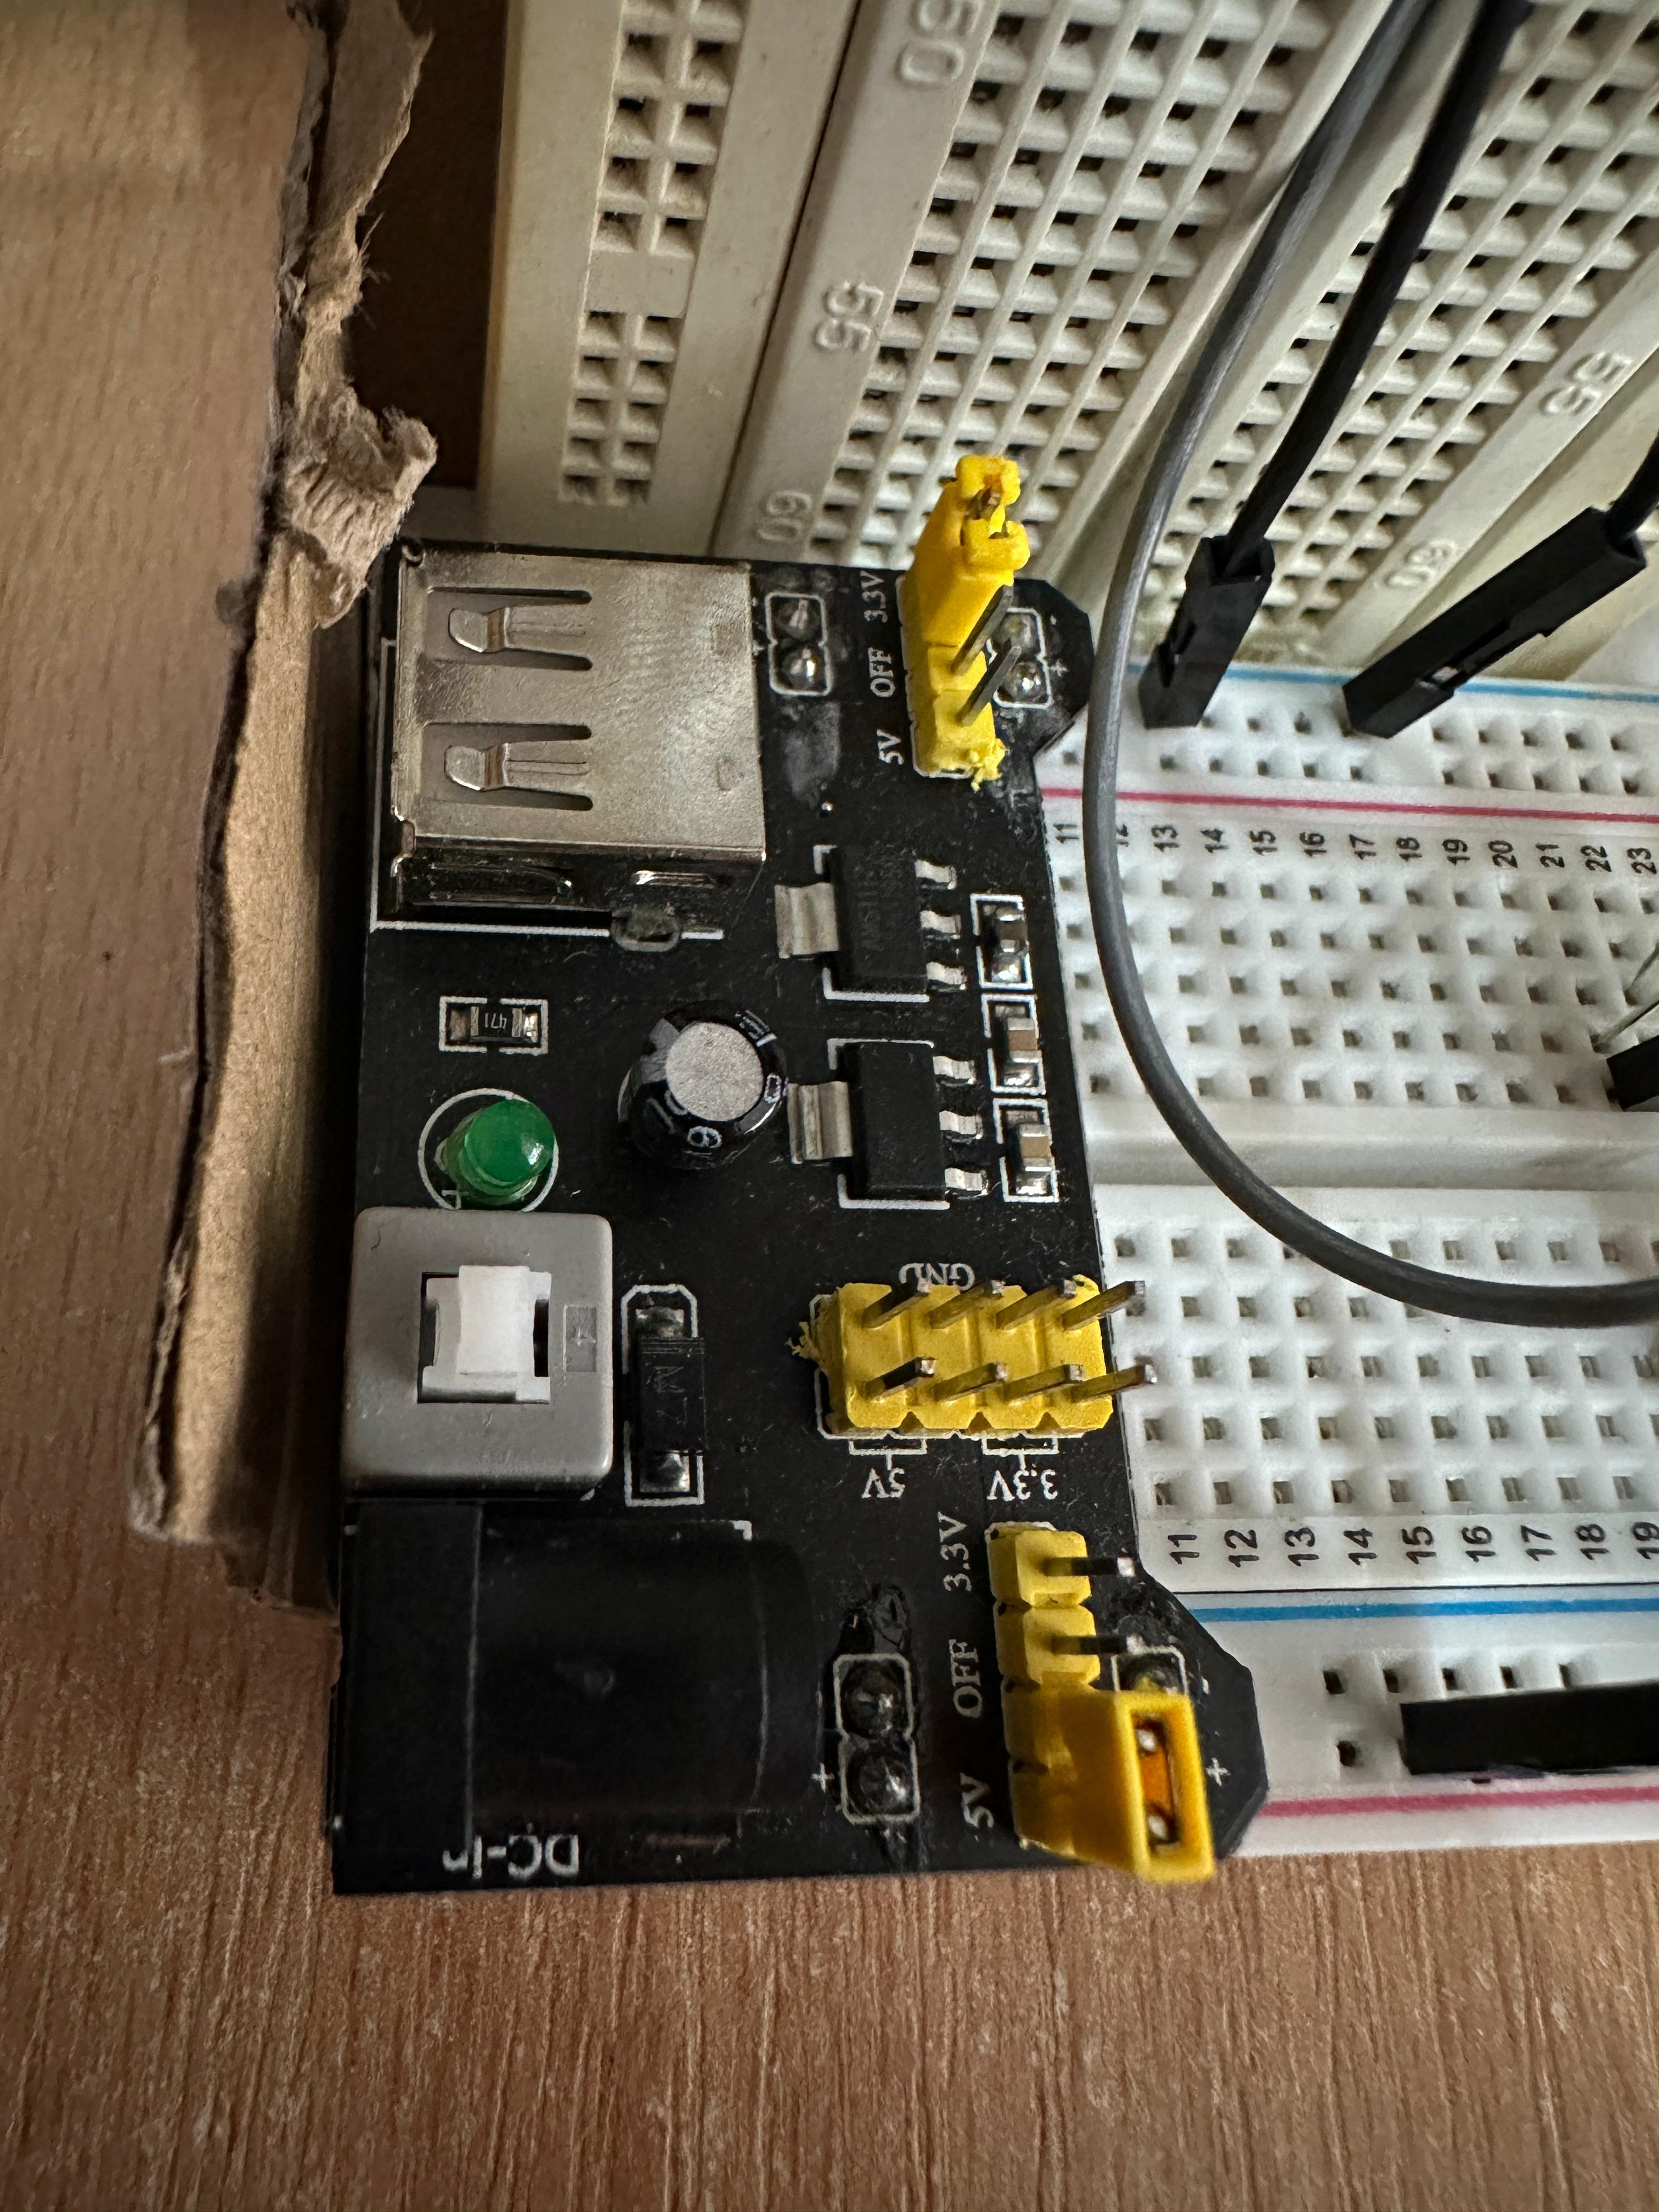
\includegraphics[width=0.3\textwidth]{power_supply.jpg}
    \caption{Modul sursă de alimentare pentru BreadBoard}
    \label{fig:power_supply}
\end{figure}
\newpage
\vspace*{1cm}
\subsection*{Aplicații pentru studenți}
\begin{itemize}
    \item \textbf{Pași pentru implementare: } 
        \begin{itemize}
        \item Conectează modulul sursă de alimentare externă la breadboard.
        \item Configurează modulul pentru a furniza 5V (sau 3.3V dacă este necesar)
        \item Conectarea semnalelor +5V de la dispozitevele LCD, servomotor la +5V de la sursă, cât și a împământării
        \end{itemize}
\end{itemize}
\begin{itemize}
    \item Alimentarea unui dispozitiv extern cu sursa de alimentare. Acest exercițiu implică alimentarea servomotorului sau LCD-ului folosind sursa externă și testează dacă acestea funcționează corect.
    \begin{lstlisting}
#include <Servo.h>

Servo myservo; // Creare obiect pentru servomotor

void setup() {
  myservo.attach(9); // Pinul de control al servomotorului conectat la Arduino
  myservo.write(0);  // Seteaza pozitia initiala la 0 grade
}

void loop() {
  myservo.write(90); // Misca servomotorul la 90 grade
  delay(2000);       // Asteapta 2 secunde
  myservo.write(0);  // Revine la 0 grade
  delay(2000);       // Asteapta 2 secunde
}

    \end{lstlisting}
\end{itemize}






\newpage
\vspace*{1cm}
\section{Conexiuni și verificare finală}
După montarea componentelor conform schemei din \textbf{Figura \ref{fig:schema_montaj}}, conexiunile trebuie verificate pentru a preveni erori:
\begin{itemize}
    \item Verificați alimentarea componentelor pentru tensiuni corecte.
    \item Confirmați că fiecare pin al Arduino este conectat corespunzător cu componentele, pentru a identifica și izola eventualele erori.
    \item Testați funcționarea sistemului pornind de la fiecare componentă individuală.
    \item Verificați stabilitatea conexiunilor de pe breadboard, asigurându-vă că firele sunt bine inserate și nu există contacte slabe care ar putea cauza funcționarea instabilă a circuitului.
    \item Monitorizați funcționarea prin intermediul consolei seriale Arduino, pentru a identifica și depana rapid eventualele erori de comunicare sau comportamente neașteptate.
    \item Efectuați o verificare vizuală finală, căutând fire inversate sau conectate greșit care ar putea provoca scurtcircuite sau comportamente necorespunzătoare.
\end{itemize}
\chapter{Rezolvare aplicații pentru studenți}
\subsection{Arduino Uno}
\begin{itemize}
    \item Controlul unui LED pentru a învăța cum să folosească pinii digitali ai Arduino.
        \begin{itemize}
            \item Înainte de toate, asigurați-vă că firul a fost mutat de pe pinul 11, pe pinul 8.
            \item Acestea sunt apoi valorile care trebuie completate pentru a duce cerința la capat:
                \begin{lstlisting}
 // Definirea pinului la care este conectat LED-ul
const int ledPin = 8; // Pinul digital 8

void setup() {
  pinMode(ledPin, OUTPUT); // Seteaza pinul LED-ului ca iesire
}

void loop() {
  digitalWrite(ledPin, HIGH); // Aprinde LED-ul
  delay(1000);               // Asteapta 1 secunda (1000 ms)
  digitalWrite(ledPin, LOW);  // Stinge LED-ul
  delay(1000);               // Asteapta 1 secunda (1000 ms)
}

                \end{lstlisting}
                \item Explicații:
                    \begin{itemize}
                        \item const int ledPin = 8; : Specifică pinul digital 8 ca fiind cel la care este conectat LED-ul
                        \item pinMode(ledPin, OUTPUT);: Setează pinul 8 ca ieșire, astfel încât să poată controla LED-ul
                        \item digitalWrite(ledPin, HIGH);: Trimite un semnal de 5V pe pinul 8, aprinzând LED-ul
                        \item delay(1000);: Introduce o întârziere de 1000 ms (1 secundă)
                        \item digitalWrite(ledPin, LOW);: Stinge LED-ul, oprind semnalul pe pinul 8.
                        \item delay(1000);: Introduce o altă întârziere de 1 secundă, creând ciclul de aprindere/stingere
                    \end{itemize}
                    
        \end{itemize}
        \item Numără de la 0 la 10, incrementând la fiecare secundă, și afișează valorile în monitorul serial.
        \begin{itemize}
            \item Completări:
                \begin{lstlisting}
// Variabila pentru a stoca valoarea curenta
int counter = 0;

void setup() {
  Serial.begin(115200); // Initializeaza comunicarea seriala la o viteza de baud rate de 115200
}

void loop() {
  if (counter <= 10) { // Verifica daca numaratoarea este pana la 10
    Serial.print("Numar: "); // Afiseaza textul
    Serial.println(counter); // Afiseaza valoarea curenta a numaratorii
    counter++; // Incrementeaza valoarea cu 1
    delay(1000); // Asteapta 1 secunda (1000 milisecunde)
  } else {
    // Opreste numaratoarea dupa 10
    Serial.println("Numaratoarea s-a terminat!");
    while (true); // Blocheaza executia intr-o bucla infinita
  }
}

                \end{lstlisting}
               
                    \item Explicații:
                        \begin{itemize}
                            \item Serial.begin(115200); : Inițializează comunicarea serială cu o viteză de baud de 115200, o rată mai rapidă utilizată frecvent pentru proiecte mai complexe sau pentru transferuri rapide de date. Această rată se va utiliza pe tot parcursul proiectului, de aceea trebuie sa vă obișnuiți încă de la început cu folosirea ei
                            \item if (counter <= 10) : Verifică dacă numărătoarea a ajuns până la 10
                            \item Serial.print("Numar: "); : Afișează textul descriptiv „Numar:” în monitorul serial
                            \item Serial.println(counter); : Afișează valoarea curentă a variabilei counter
                            \item counter++; : Crește valoarea variabilei counter cu 1.
                            \item delay(1000); : Introduce o întârziere de 1 secundă între afișări
                            \item else : Dacă counter este mai mare decât 10, afișează mesajul „Numaratoarea s-a terminat!” și intră într-o buclă infinită pentru a opri programul
                            
                        \end{itemize}
             
        \end{itemize}

\end{itemize}
\subsection{ESP32-CAM} 
Pentru partea de ESP32-CAM sunt oferite toate indicațiile încă de la partea de exerciții, fiind câteva instrucțiuni de urmat pentru familiarizarea cu modul în care funcționează plăcuța.

\subsection{Motor servo MG996R}
\begin{itemize}
    \item Mișcă servo-ul între 0° și 180° cu pauză
    \begin{itemize}
        \item Completări:
            \begin{lstlisting}
 #include <Servo.h>

Servo myServo;            // Cream un obiect Servo pentru a controla motorul
const int servoPin = 9;   // Pinul la care este conectat servo-ul in configuratie

void setup() {
  myServo.attach(servoPin); // Atasam pinul servo-ului
}

void loop() {
  // Misca servo-ul de la 0° la 180°
  for (int pos = 0; pos <= 180; pos++) {
    myServo.write(pos);   // Seteaza pozitia servo-ului
    delay(15);            // Pauza pentru a permite motorului sa se miste
  }

  delay(1000);            // Pauza 1 secunda
   \end{lstlisting}
   \newpage
   \vspace*{1cm}
   \begin{lstlisting}
  // Misca servo-ul inapoi de la 180° la 0°
  for (int pos = 180; pos >= 0; pos--) {
    myServo.write(pos);
    delay(15);
  }

  delay(1000);            // Pauza 1 secunda
}

            \end{lstlisting}
        \item Explicații:
            \begin{itemize}
                \item const int servoPin = 9; : Pinul digital 9 este folosit pentru controlul servomotorului (în funcție de configurația ta, poate fi schimbat)
                \item Mișcarea servo-ului între 0° și 180° : for (int pos = 0; pos <= 180; pos++) : Mișcă servo-ul de la poziția 0° la 180°. ; delay(15); : Introduce o pauză de 15 ms pentru a permite servo-ului să se miște la următoarea poziție.
                \item Mișcarea servo-ului înapoi între 180° și 0° : for (int pos = 180; pos >= 0; pos- -): Mișcă servo-ul de la poziția 180° la 0°
                \item Pauzele dintre mișcări: delay(1000); : O pauză de 1 secundă este adăugată între ciclurile de mișcare pentru a observa clar schimbarea.
            \end{itemize}
            
    \end{itemize}
    \item Mișcă servo-ul în funcție de mesajul primit de la LCD
    \begin{itemize}
        \item Completări: 
        \begin{lstlisting}
#include <Servo.h>
#include <Wire.h>
#include <LiquidCrystal_I2C.h>

// Obiecte pentru servomotor si LCD
Servo myservo;
LiquidCrystal_I2C lcd(0x27, 16, 2); // Adresa LCD-ului I2C

// Variabile globale
bool isAccessGranted = false; // Flag pentru acces

void setup() {
  Serial.begin(115200); // Initializare conexiune seriala
  myservo.attach(9); // Ataseaza pinul de control al servomotorului
\end{lstlisting}
\newpage
\vspace*{1cm}
\begin{lstlisting}
  myservo.write(0); // Seteaza pozitia initiala a servomotorului

  lcd.init();
  lcd.backlight();
  lcd.clear();
  lcd.print("Sistem pornit"); // Mesajul initial pe LCD
  delay(2000);
  lcd.clear();
}

void loop() {
  if (Serial.available() > 0) {
    String message = Serial.readStringUntil('\n'); // Citire mesaj serial

    if (message == "PERMIS") {
      isAccessGranted = true;
      lcd.clear();
      lcd.print("Acces permis");
      myservo.write(90); // Pozitia pentru acces permis
    } else if (message == "RESPINS") {
      isAccessGranted = false;
      lcd.clear();
      lcd.print("Acces respins");
      myservo.write(0); // Revine la pozitia initiala
    }
  }
}

        \end{lstlisting}
        
    \end{itemize}
    
\end{itemize}

\subsection{LCD 16x2 cu I2C}
\begin{itemize}
    \item Afișarea unui mesaj static, precum ”Bun venit!”.
    \begin{itemize}
        \item Completări cod:
            \begin{lstlisting}
#include <Wire.h>
#include <LiquidCrystal_I2C.h>
\end{lstlisting}
\newpage
\vspace*{1cm}
\begin{lstlisting}

// Initializare LCD cu adresa I2C
LiquidCrystal_I2C lcd(0x27, 16, 2); // Adresa poate fi diferita (verificati in functie de modulul vostru)

void setup() {
  lcd.init();           // Initializare LCD
  lcd.backlight();      // Activeaza iluminarea de fundal
  lcd.clear();          // Curata ecranul
  lcd.print("Bun venit!"); // Afiseaza mesajul "Bun venit!"
}

void loop() {
  // Bucla principala nu face nimic
}

            \end{lstlisting}
            \item Explicații:
            \begin{itemize}
                \item lcd.init(); : Inițializează LCD-ul pentru a-l putea folosi
                \item lcd.backlight(); : Activează iluminarea de fundal pentru o vizibilitate mai bună
                \item lcd.clear(); : Curăță orice informație anterioară afișată pe LCD
                \item lcd.print("Bun venit!"); : Afișează mesajul static „Bun venit!” pe LCD.
            \end{itemize}
    \end{itemize}
    \item Afișarea accesului permis sau respins
    \begin{itemize}
        \item Completări cod:
            \begin{lstlisting}
#include <Servo.h>
#include <Wire.h>
#include <LiquidCrystal_I2C.h>

// Obiecte pentru servomotor si LCD
Servo myservo;
LiquidCrystal_I2C lcd(0x27, 16, 2); // Adresa LCD-ului I2C

// Variabile globale
bool isAccessGranted = false; // Flag pentru acces
\end{lstlisting}
\newpage
\vspace*{1cm}
\begin{lstlisting}
    


void setup() {
  Serial.begin(115200);     // Initializare conexiune seriala
  myservo.attach(9);        // Pinul de semnal pentru servomotor
  myservo.write(0);         // Pozitia initiala a servomotorului
  lcd.init();               // Initializare LCD
  lcd.backlight();          // Activeaza iluminarea de fundal
  lcd.clear();
  lcd.print("Asteptare..."); // Afiseaza mesajul "Asteptare..."
}

void loop() {
  if (Serial.available() > 0) {
    String message = Serial.readStringUntil('\n'); // Citire mesaj
    if (message == "PERMIS") {
      isAccessGranted = true;
      lcd.clear();
      lcd.print("Acces permis"); // Afiseaza mesajul "Acces permis"
      Serial.println("Acces permis");
    } else if (message == "RESPINS") {
      isAccessGranted = false;
      lcd.clear();
      lcd.print("Acces respins"); // Afiseaza mesajul "Acces respins"
      Serial.println("Acces respins");
    } else {
      lcd.clear();
      lcd.print("Mesaj necunoscut"); // Afiseaza mesajul "Mesaj necunoscut"
      Serial.println("Mesaj necunoscut primit");
    }
  }
\end{lstlisting}
\newpage
\vspace*{1cm}
\begin{lstlisting}
  // Miscare servomotor daca accesul este permis
  if (isAccessGranted) {
    myservo.write(90);      // Deschide servomotorul
    delay(2000);            // Asteapta 2 secunde
    myservo.write(0);       // Inchide servomotorul
    isAccessGranted = false; // Reseteaza flag-ul
  }
}

            \end{lstlisting}
            \item Explicații:
                \begin{itemize}
                    \item Inițializare conexiune serială: Serial.begin(115200); Necesită un baud rate rapid pentru comunicare serială
                    \item myservo.write(0); Asigură că motorul începe din poziția de bază
                    \item Mesaje afișate pe LCD: Mesaje relevante sunt afișate pentru stări diferite
                    \item delay(2000); myservo.write(0); : Mișcarea motorului 

                \end{itemize}
    \end{itemize}
    
\end{itemize}

\subsection{LED-uri}
\begin{itemize}
    \item  Crearea unui semnal intermitent (blink) pentru un LED
    \begin{itemize}
        \item Completări cod:
            \begin{lstlisting}
  void setup() {
  pinMode(ledGreen, OUTPUT); // Configureaza LED-ul verde ca iesire
}

void loop() {
  digitalWrite(ledGreen, HIGH); // Aprinde LED-ul verde
  delay(500);                   // Asteapta 500 ms
  digitalWrite(ledGreen, LOW);  // Stinge LED-ul verde
  delay(500);                   // Asteapta 500 ms
}

            \end{lstlisting}
            \newpage 
            \vspace*{1cm}
            \item Explicații: 
                \begin{itemize}
                    \item pinMode(ledGreen, OUTPUT);   Configurează pinul ledGreen ca ieșire
                    \item digitalWrite(ledGreen, HIGH);   Aprinde LED-ul verde trimițând semnal de 5V
                    \item digitalWrite(ledGreen, LOW);   Stinge LED-ul verde oprind semnalul
                    \item delay(500);   Introduce o pauză de 500 ms între aprindere și stingere
                \end{itemize}
    \end{itemize}
    \item Aprinderea LED-urilor în funcție de accesul permis sau respins
    \begin{itemize}
        \item Completare cod:
            \begin{lstlisting}
  void setup() {
  pinMode(ledGreen, OUTPUT); // Configureaza LED-ul verde ca iesire
  pinMode(ledRed, OUTPUT);   // Configureaza LED-ul rosu ca iesire
  Serial.begin(115200);      // Porneste comunicatia seriala
}

void loop() {
  if (Serial.available() > 0) {
    String message = Serial.readStringUntil('\n'); // Citeste mesajul trimis prin serial

    if (message == "PERMIS") {
      digitalWrite(ledGreen, HIGH); // Aprinde LED-ul verde
      digitalWrite(ledRed, LOW);    // Stinge LED-ul rosu
      Serial.println("Acces permis: LED verde aprins");
    } else if (message == "RESPINS") {
      digitalWrite(ledGreen, LOW);  // Stinge LED-ul verde
      digitalWrite(ledRed, HIGH);  // Aprinde LED-ul rosu
      Serial.println("Acces respins: LED rosu aprins");
    } else {
      digitalWrite(ledGreen, LOW); // Stinge ambele LED-uri
      \end{lstlisting}
      \begin{lstlisting}
      digitalWrite(ledRed, LOW);
      Serial.println("Mesaj necunoscut: Ambele LED-uri stinse");
    }
  }
}

            \end{lstlisting}
            \item Explicații: 
                \begin{itemize}
                    \item pinMode(ledRed, OUTPUT);   Configurează pinul ledRed ca ieșire
                    \item Serial.begin(115200);   Inițializează comunicația serială pentru transmiterea și recepția mesajelor
                    \item digitalWrite(ledGreen, HIGH);   Aprinde LED-ul verde pentru „PERMIS”
                    \item digitalWrite(ledRed, HIGH);   Aprinde LED-ul roșu pentru „RESPINS”
                    \item digitalWrite(ledGreen, LOW); și digitalWrite(ledRed, LOW);   Sting ambele LED-uri în caz de mesaj necunoscut
                \end{itemize}
    \end{itemize}
\end{itemize}

\subsection{Potențiometru}
\begin{itemize}
    \item Reglarea luminozității unui LED prin citirea poziției potentiometrului.
        \begin{itemize}
            \item Comlpetare cod:
                \begin{lstlisting}
 const int potentiometerPin = A0; // Pin pentru potentiometru
const int ledGreen = 12;        // Pin pentru LED verde
const int ledRed = 11;          // Pin pentru LED rosu

void setup() {
  pinMode(ledGreen, OUTPUT);    // Configureaza LED-ul verde ca iesire
  pinMode(ledRed, OUTPUT);      // Configureaza LED-ul rosu ca iesire
  Serial.begin(115200);         // Porneste comunicatia seriala
}

void loop() {
  int potValue = analogRead(potentiometerPin); // Citeste valoarea analogica de la potentiometru
  int ledIntensity = map(potValue, 0, 1023, 0, 255); // Mapare valoare 0-1023 la 0-255
  \end{lstlisting}
  \newpage
  \vspace*{1cm}
  \begin{lstlisting}
  analogWrite(ledGreen, ledIntensity); // Ajusteaza intensitatea LED-ului verde
  analogWrite(ledRed, 255 - ledIntensity); // Ajusteaza intensitatea LED-ului rosu

  delay(1000); // Pauza scurta pentru stabilitate
}

                \end{lstlisting}
                \item Explicații:
                    \begin{itemize}
                        \item analogRead(potentiometerPin)   Citește valoarea analogică de la potențiometru (0-1023)
                        \item map(potValue, 0, 1023, 0, 255)   Transformă valoarea într-un interval corespunzător intensității LED-ului (0-255)
                        \item analogWrite(ledGreen, ledIntensity)   Ajustează luminozitatea LED-ului verde în funcție de poziția potențiometrului
                        \item analogWrite(ledRed, 255 - ledIntensity)   Inversează luminozitatea pentru LED-ul roșu, astfel încât doar unul dintre LED-uri să fie mai luminos.
                    \end{itemize}
        \end{itemize}
        \item  Citirea valorii analogice de la potențiometru și afișarea acesteia pe monitorul serial
            \begin{itemize}
                \item Completare cod:
                    \begin{lstlisting}
const int potentiometerPin = A0; // Pin pentru potentiometru

void setup() {
  Serial.begin(115200); // Porneste comunicatia seriala
}

void loop() {
  int potValue = analogRead(potentiometerPin); // Citeste valoarea analogica de la potentiometru

  Serial.print("Valoare potentiometru: "); // Afiseaza textul descriptiv
  \end{lstlisting}
  \newpage
  \vspace*{1cm}
  \begin{lstlisting}
  Serial.println(potValue);               // Afiseaza valoarea citita

  delay(500);                             // Pauza de 500 ms pentru stabilitate
}

                    \end{lstlisting}
                    \item Explicații: 
                        \begin{itemize}
                            \item analogRead(potentiometerPin)   Citește valoarea analogică de la potențiometru (0-1023)
                            \item Serial.print("Valoare potențiometru: ");   Afișează un text descriptiv pe monitorul serial
                            \item Serial.println(potValue); → Afișează valoarea numerică citită de la potențiometru
                            \item delay(500); → Asigură o pauză între afișări pentru stabilitate.
                            
                        \end{itemize}
            \end{itemize}
            
\end{itemize}

\chapter{Desfășurarea lucrării - partea 2}
Recomandăm instalarea versiunii de Arduino 1.8.18, deoarece prezintă suport mai bun pentru comunicarea cu ESP32-CAM.
\section{Biblioteci necesare}
Se instalează bibliotecele atașate:
\begin{figure}[H]
    \centering
    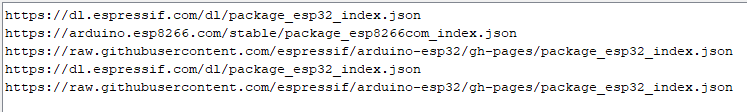
\includegraphics[width=1\textwidth]{biblioteci.png}
    \caption{Biblioteci Arduino}
    \label{fig:biblioteci}
\end{figure}
Mai întâi se încară exemplul de CameraWebServer, care poate fi găsit la File->Examples-ESP32->Camera, după ce bibliotecile au fost instalate cu succes, acest exemplu va apărea după ce la tools selectăm ESP32 Wrover Module. Ne asiguram ca toate define-urile din cod sunt comentate mai putin cel cu : \begin{lstlisting}
#define CAMERA_MODEL_AI_THINKER // Has PSRAM
\end{lstlisting}
De asemenea trebuie să vă asigurați ca datele pentru internet sunt cele la care laptop-ul este conectat prin completarea corespunzătoare a câmpurilor:
\begin{lstlisting}
const char *ssid = "";
const char *password = "";
\end{lstlisting}
\newpage
\vspace*{1cm}
Pentru ca încărcarea codului să funționeze trebuie ca datele pentru Board sa fie cele atașate la Tools:
\begin{figure}[H]
    \centering
    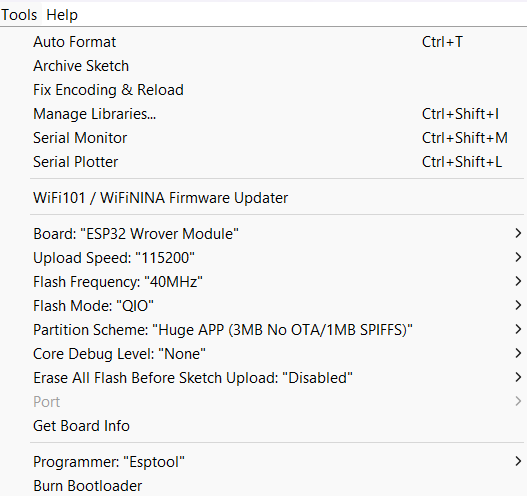
\includegraphics[width=0.6\textwidth]{cameraWebServer_tools.png}
    \caption{Configurare exemplu Camera}
    \label{fig:cameraWebServer_tools}
\end{figure}

Încărcarea corectă a codului se realizeă atunci când scrierea ajunge la 100%:
\begin{figure}[H]
    \centering
    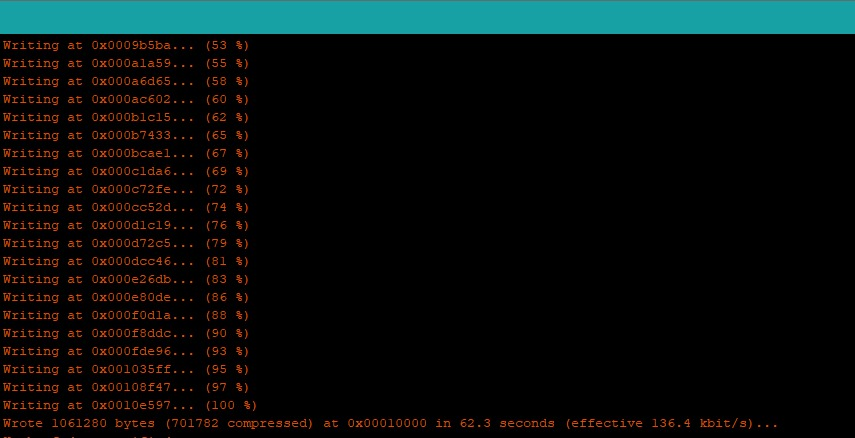
\includegraphics[width=0.8\textwidth]{scriere_data.jpg}
    \caption{Încărcare cod pe ESP}
    \label{scriere_data}
\end{figure} 

La finalizarea execuției se scoate firul dintre GPIO și GND de pe ESP, pentru a scoate placa din modul de programare, se deschide Serial Monitor și se apasă butonul de reset al plăcuței. Conexiunea se realizează atunci când apare:
\newpage
\vspace*{1cm}
\begin{figure}[H]
    \centering
    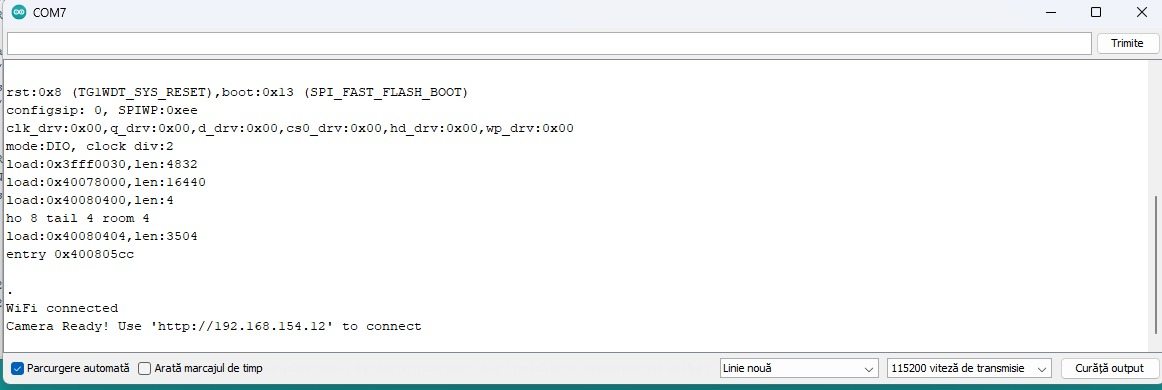
\includegraphics[width=1\textwidth]{confirmare_conexiune.jpg}
    \caption{Confirmare conectare ESP}
    \label{confirmare_conexiune}
\end{figure} 

Se poate testa funcționalitatea camerei prin accesarea url-ului, astfel deschizându-se interfața de le Espressif:
\begin{figure}[H]
    \centering
    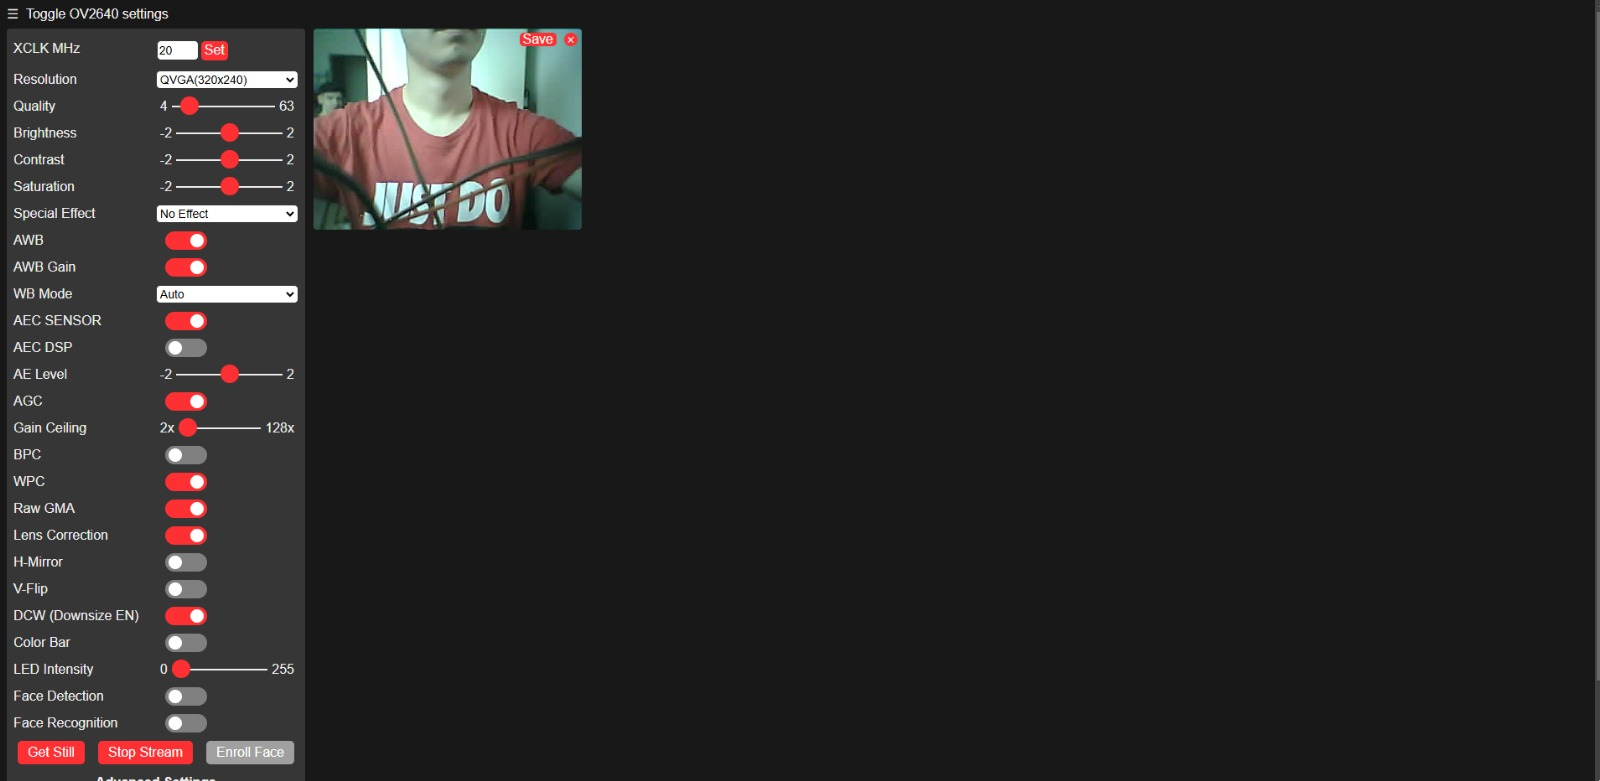
\includegraphics[width=1\textwidth]{interfata_ESP.jpg}
    \caption{Interfața ESP}
    \label{interfata_ESP}
\end{figure} 

\section{Programare cu biblioteci Arduino}

Codul este împărțit în mai multe secțiuni. Anumite părți ale codului sunt lăsate incomplete, iar comentariile indică clar ce trebuie implementat de către studenți.

1. Inițializarea componentelor
Se inițializează conexiunile și componentele hardware. Studenții trebuie să completeze inițializarea pinilor LED și poziția inițială a servomotorului.
\newpage
\vspace*{1cm}
\begin{lstlisting}[language=C++]
// Initializare conexiune seriala si componente hardware
Serial.begin(115200);
myservo.attach(10);      // Pinul pentru servomotor
myservo.write(???);     // ??? - Stabiliti pozitia initiala a servomotorului (0-180°)

// Initializare pinii LED
pinMode(ledGreen, ???); // ??? - Configurati pinul LED-ului verde ca OUTPUT
pinMode(ledRed, ???);   // ??? - Configurati pinul LED-ului rosu ca OUTPUT

lcd.init();             // Initializare LCD
lcd.backlight();
lcd.print("Sistem pornit"); // Mesaj initial
delay(2000); 
lcd.clear();
Serial.println("Sistem Arduino porint. Astept mesaje...");
\end{lstlisting}

### 2. Procesarea mesajelor primite
Mesajele primite prin Serial Monitor sunt utilizate pentru a controla accesul. Studenții trebuie să completeze funcționalitățile pentru a reseta servomotorul și pentru a implementa o acțiune suplimentară.

\begin{lstlisting}[language=C++]
if (Serial.available() > 0) {
  String message = Serial.readStringUntil('\n');

  if (message == "PERMIS") {
    isAccessGranted = ???;  // ??? - Seteaza flag-ul pentru acces permis
    lcd.clear();
    lcd.print("Acces permis");
  } else if (message == "RESPINS") {
    isAccessGranted = ???;  // ??? - Resetati flag-ul pentru acces respins
    myservo.write(???);     // ??? - Pozitionati servomotorul in pozitia de start
    lcd.clear();
    lcd.print("Acces respins");
  }
}
\end{lstlisting}

\vspace*{1cm}
### 3. Controlul servomotorului
Codul controlează mișcarea servomotorului dacă accesul este permis. Studenții trebuie să ajusteze logica pentru inversarea direcției și să adauge o limitare la o anumită poziție.

\begin{lstlisting}[language=C++]
if (isAccessGranted) {
  static int pos = 0;             // Pozitia curenta a motorului
  static bool direction = true;  // Directia de miscare

  if (direction) {
    pos += ???;  // ??? - Stabiliti pasul de crestere a pozitiei
    if (pos >= ???) direction = false; // ??? - Inverseaza directia la limita
  }
else {
    pos -= ???;  // ??? - Stabiliti pasul de descrestere a pozitiei


    if (pos <= ???) direction = true; // ??? - Inverseaza directia la pozitia initiala
  }

  myservo.write(pos); // Seteaza pozitia servomotorului
  delay(15);          // Intarziere pentru miscare lina
}
\end{lstlisting}

### 4. Citirea potențiometrului și controlul LED-urilor
Se reglează intensitatea LED-urilor pe baza valorii citite de la potențiometru. Studenții trebuie să implementeze maparea valorilor pentru PWM și controlul LED-urilor în funcție de starea accesului.

\begin{lstlisting}[language=C++]
// Citire valoare potențiometru
int potValue = analogRead(potentiometerPin); // 0-1023
int ledIntensity = ???;                      // ??? - Mapare valoare potentiometru la intervalul 0-255

if (isAccessGranted) {
  analogWrite(ledGreen, ???); // ??? - Controlati intensitatea LED verde
  analogWrite(ledRed, 0);     // ??? - Opriti LED-ul rosu
} else {
  analogWrite(ledRed, ???);   // ??? - Controlati intensitatea LED rosu
  \end{lstlisting}
  \vspace*{1cm}
  \begin{lstlisting}
  analogWrite(ledGreen, 0);   // ??? - Opriti LED-ul verde
}
\end{lstlisting}

### 5. Testare finală
Studenții trebuie să testeze și să completeze implementările din cod. Pași sugerați pentru testare:
- Trimiteți mesaje din Serial Monitor (\texttt{PERMIS} și \texttt{RESPINS}) și observați mișcarea servomotorului.
- Reglați potențiometrul și verificați intensitatea LED-urilor.
- Verificați pozițiile limită ale servomotorului.

Acest exercițiu le permite studenților să implementeze funcționalitățile lipsă și să înțeleagă mai bine programarea componentelor hardware cu Arduino.

\newpage
\vspace*{1cm}
\section{Programare pe registri pentru controlul servomotorului}

Pentru implementarea funcționalității servomotorului, în locul utilizării bibliotecii `Servo.h`, vom folosi controlul direct al timer-ului 1 pe microcontrolerul ATmega328P, conform documentației acestuia. Timer-ul va fi configurat pentru a genera semnalul PWM necesar motorului MG996R.

\subsection*{Configurația PWM pe registri}

\begin{figure}[H]
    \centering
    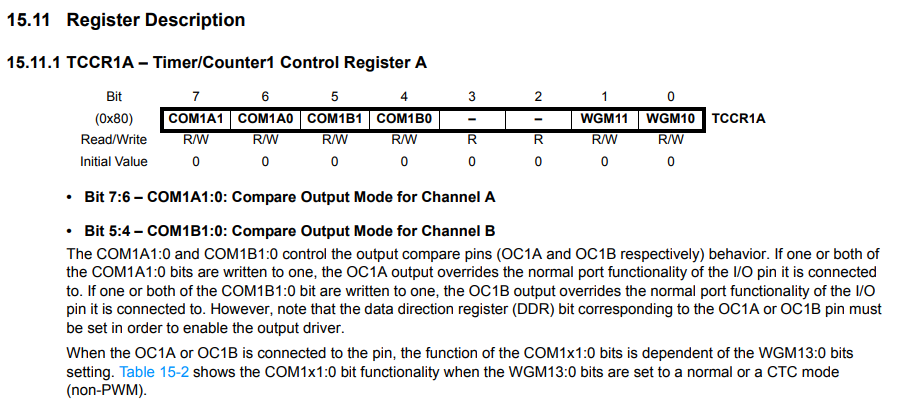
\includegraphics[width=0.8\textwidth]{tccr1a.png}
    \caption{ TCCR1A – Timer/Counter1 Control Register A}
    \label{fig:TCCR1A}
\end{figure}

\begin{itemize}
    \item COM1A1 și COM1A0 (Compare Output Mode for Channel A): Neutilizate în configurația noastră, deoarece folosim canalul B (OC1B) pentru generarea PWM
    \item COM1B1 și COM1B0 (Compare Output Mode for Channel B):
        \begin{itemize}
            \item Configurația este setată pentru Clear on Compare Match: OC1B este setat la HIGH la începutul ciclului și trece la LOW atunci când contorul ajunge la valoarea din OCR1B 
            \item Din \textbf{Figura \ref{fig:FastPwm}}, configurăm:
                \begin{itemize}
                    \item COM1B1 = 1, COM1B0 = 0   Clear OC1B on Compare Match (mod non-inverting)
                \end{itemize}
            \item WGM11 și WGM10 (Waveform Generation Mode): Modul Fast PWM cu TOP în ICR1 necesită setarea WGM11 = 1 și WGM10 = 0 în acest registru.
            \item Logica alegerii bitilor: 
            \begin{itemize}
                \item COM1B1 = 1 și COM1B0 = 0 au fost alese pentru generarea unui semnal PWM în mod non-inverting, ideal pentru controlul precis al servomotorului.
                \item WGM11 = 1 și WGM10 = 0 au fost necesare pentru configurarea modului Fast PWM cu valori configurabile de TOP
            \end{itemize}
            
        \end{itemize}
        \item (1 << COM1B1): Activează modul non-inverting pentru canalul B
        \item (1 << WGM11): Activează partea de configurare pentru modul Fast PWM
\end{itemize}

\begin{figure}[H]
    \centering
    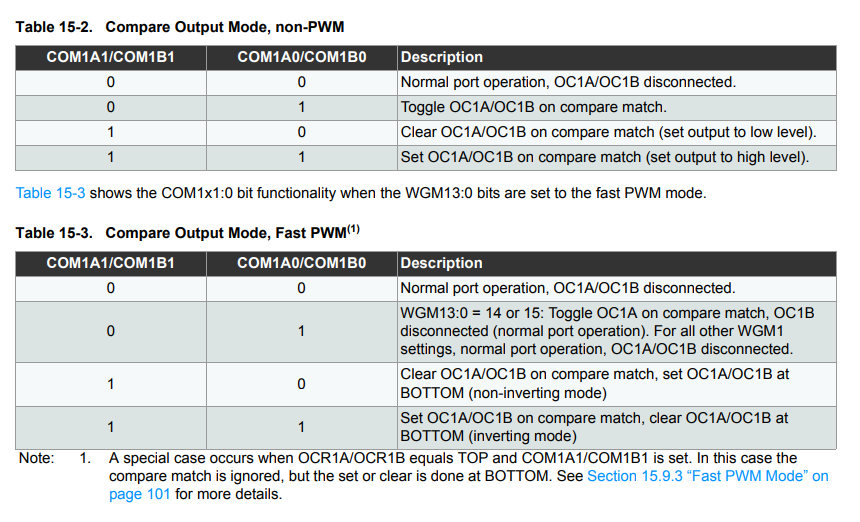
\includegraphics[width=0.8\textwidth]{NONpwm&PWM.png}
    \caption{Compare Output Mode, Fast PWM}
    \label{fig:FastPwm}
\end{figure}
\begin{itemize}
    \item Pentru Fast PWM, folosim modul în care OC1B este setat pe CLEAR la Compare Match și SET la BOTTOM
    \item Această configurație este indicată prin COM1B1 = 1 și COM1B0 = 0
\end{itemize}
\newpage
\vspace*{1cm}
\begin{figure}[H]
    \centering
    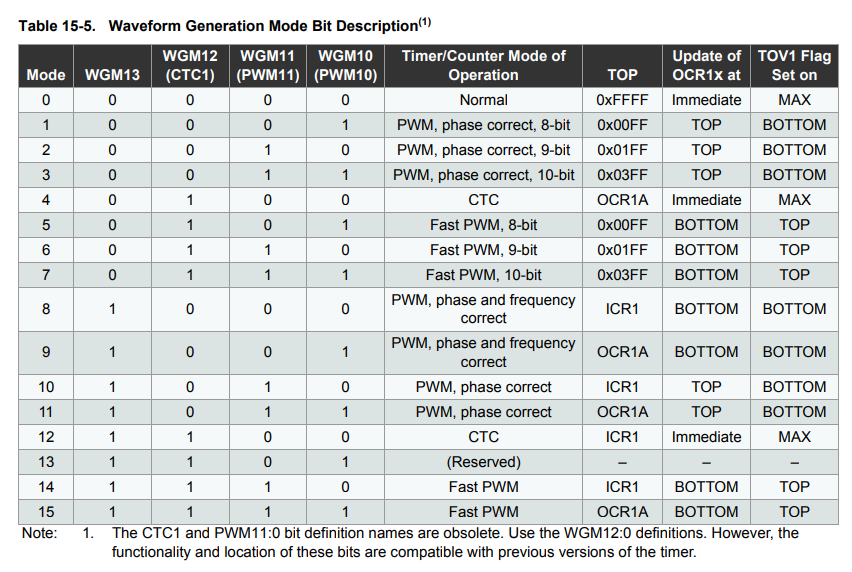
\includegraphics[width=0.8\textwidth]{waveformGeneration.png}
    \caption{Waveform Generation Mode Bit Description}
    \label{fig:waveform}
\end{figure}

\textbf{Modul Fast PWM cu TOP în ICR1 este identificat de:}
 \begin{itemize}
     \item WGM13 = 1, WGM12 = 1, WGM11 = 1, WGM10 = 0.
 \end{itemize}

 \textbf{Logica alegerii modului:}
 \begin{itemize}
     \item Modul Fast PWM cu TOP definit de ICR1 este ideal pentru generarea unui semnal precis la frecvența de 50 Hz necesară servomotorului
     \item Alegerea bitilor permite flexibilitatea în configurarea frecvenței și a duratei impulsurilor
     \item (1 << WGM13) | (1 << WGM12): Activează modul Fast PWM cu TOP în ICR1
     \item (1 << CS11): Selectează prescaler-ul de 8 pentru Timer1
 \end{itemize}
\newpage
\vspace*{1cm}
 \begin{figure}[H]
    \centering
    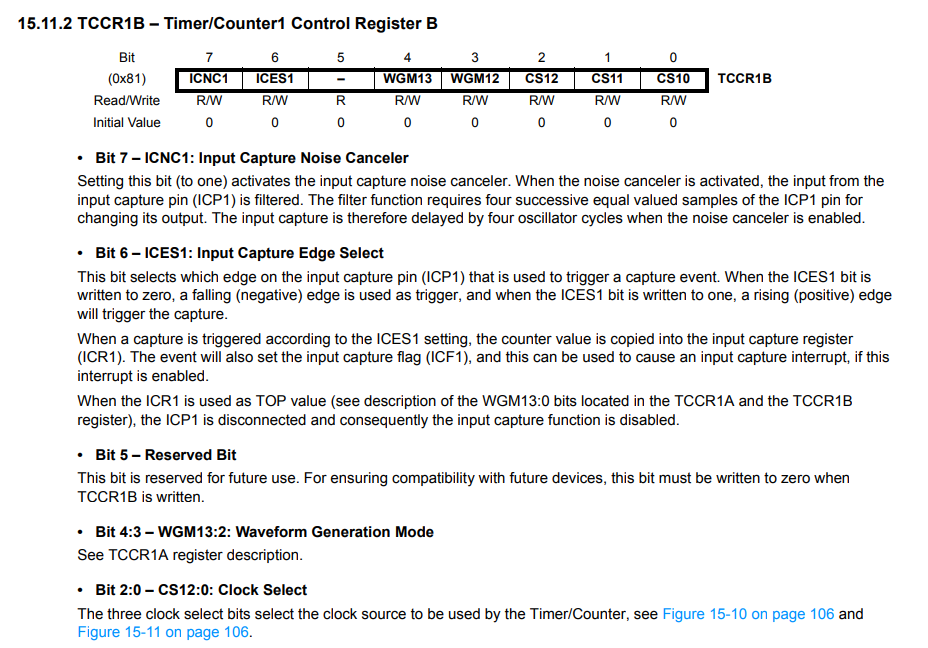
\includegraphics[width=0.8\textwidth]{tccr1B.png}
    \caption{TCCR1B – Timer/Counter1 Control Register B}
    \label{fig:TCCR1B}
\end{figure}

\begin{itemize}
    \item WGM13 și WGM12: Activează modul Fast PWM cu TOP definit de ICR1, completând configurarea din TCCR1A
    \item CS12:0 (Clock Select): Am selectat CS11 = 1 pentru un prescaler de 8, reducând frecvența ceasului sistemului pentru a obține semnalul de 50 Hz
    \item Logica alegerii bitilor:
        \begin{itemize}
            \item CS11 = 1 reduce frecvența ceasului sistemului la o valoare potrivită pentru generarea PWM
            \item WGM13 și WGM12 = 1 completează modul Fast PWM
        \end{itemize}
    \item TCCR1B = (1 << WGM13) | (1 << WGM12) | (1 << CS11); Activează modul PWM cu prescaler de 8

\end{itemize}

\textbf{ICR1 – Input Capture Register 1:} Acest registru definește valoarea TOP pentru Timer1 în modul Fast PWM.
ICR1 = 39999; // Perioadă de 20 ms pentru PWM de 50 Hz

\textbf{ OCR1B – Output Compare Register 1B:} Acest registru definește durata impulsului PWM pentru controlul servomotorului.
\begin{itemize}
    \item OCR1B = 3000; // Semnal neutru
    \item OCR1B = 2000; // Poziție minimă
    \newpage 
    \vspace*{1cm}
    \item OCR1B = 4000; // Poziție maximă
\end{itemize}
\section*{Calculul valorilor}

\subsection*{Semnal neutru (1.5 ms):}
\[
OCR1B = \frac{1.5 \times 10^{-3} \times 16,000,000}{8} = 3000
\]

\subsection*{Semnal minim (1 ms):}
\[
OCR1B = \frac{1.0 \times 10^{-3} \times 16,000,000}{8} = 2000
\]

\subsection*{Semnal maxim (2 ms):}
\[
OCR1B = \frac{2.0 \times 10^{-3} \times 16,000,000}{8} = 4000
\]


\textbf{DDRB – Data Direction Register for Port B:} Configurarea pinului PB2 (OC1B) ca ieșire.\\
\texttt{DDRB |= (1 << PB2);}

Vom configura timer-ul 1 pentru a funcționa în modul \textbf{Fast PWM cu TOP în ICR1}, generând un semnal PWM de 50 Hz (perioada de 20 ms).


Formulele de calcul utilizate sunt următoarele:
\begin{itemize}
    \item Frecvența semnalului PWM: 
    \[
    f_{PWM} = \frac{f_{clk}}{\text{Prescaler} \times (\text{ICR1} + 1)}
    \]
    Unde:
    \begin{itemize}
        \item $f_{clk}$ este frecvența ceasului sistemului (16 MHz pentru Arduino Uno),
        \item \text{Prescaler} este 8,
        \item \text{ICR1} este valoarea maximă a contorului.
    \end{itemize}
    \item Perioada PWM: 
    \[
    T_{PWM} = \frac{1}{f_{PWM}}
    \]
    \item Durata impulsului „high” pentru semnalul PWM (în microsecunde): 
    \[
    OCR1B = \frac{t_{high} \times f_{clk}}{\text{Prescaler}}
    \]
    Unde $t_{high}$ este durata impulsului (1 ms - 2 ms pentru motor).
\end{itemize}
\newpage
\vspace*{1cm}
### Cod pentru configurarea registrilor
Părți ale codului sunt lăsate incomplete pentru a fi completate de studenți. Comentariile indică exact ce trebuie făcut:

\begin{lstlisting}[language=C++]
void setup() {
  // Configurare Fast PWM pe OC1B (PB2, Pin Digital 10 pe Arduino Uno)
  // TCCR1A controleaza modul de operare al Timerului 1 si setarile canalelor de iesire.
  TCCR1A = (1 << COM1B1); // ??? - Adaugati bitii necesari pentru modul Clear on Compare Match
  TCCR1A |= (1 << ???);   // ??? - Activati modul Fast PWM 

  // TCCR1B controleaza prescaler-ul si modul de operare al Timerului 1.
  TCCR1B = (1 << ???) | (1 << ???); // ??? - Activati modul Fast PWM 
  TCCR1B |= (1 << ???);             // ??? - Selectati prescaler-ul de 8 

  // ICR1 defineste valoarea TOP pentru timer in modul Fast PWM.
  ICR1 = ???;  // ??? - Calculati valoarea ICR1 pentru o perioada de 20 ms 

  // OCR1B defineste durata impulsului PWM pentru canalul B (OC1B).
  OCR1B = ???;  // ??? - Setati valoarea pentru semnalul neutru (1.5 ms)

  // Configuram pinul PB2 (OC1B, Pin Digital 10) ca iesire.
  DDRB |= (1 << ???);  // ??? - Setati PB2 ca iesire pentru semnalul PWM
}

void loop() {
  // Modificam valoarea OCR1B pentru a schimba durata impulsului PWM si pozitia servo-ului.

  // OCR1B = ???: Semnal PWM "high" timp de 1 ms.
  OCR1B = ???; // ??? - Setati valoarea pentru pozitia minima a motorului
  \end{lstlisting}
  \newpage
  \vspace*{1cm}
  \begin{lstlisting}[language=C++]
  delay(1000); // Asteapta 1 secunda inainte de urmatoarea schimbare.
  // OCR1B = ???: Semnal PWM "high" timp de 2 ms.
  OCR1B = ???; // ??? - Setati valoarea pentru pozitia maxima a motorului
  delay(1000); // Asteapta 1 secunda inainte de urmatoarea schimbare.
}
\end{lstlisting}

### Justificarea calculului registrilor
\textbf{Calcul pentru ICR1:}
\[
ICR1 = \frac{f_{clk}}{\text{Prescaler} \times f_{PWM}} - 1 = \frac{16,000,000}{8 \times 50} - 1 = 39,999
\]

\textbf{Calcul pentru OCR1B:}
\begin{itemize}
    \item Pentru semnalul neutru (1.5 ms): 
    \[
    OCR1B = \frac{1.5 \times 10^{-3} \times 16,000,000}{8} = 3000
    \]
    \item Pentru semnalul minim (1 ms): 
    \[
    OCR1B = \frac{1.0 \times 10^{-3} \times 16,000,000}{8} = 2000
    \]
    \item Pentru semnalul maxim (2 ms): 
    \[
    OCR1B = \frac{2.0 \times 10^{-3} \times 16,000,000}{8} = 4000
    \]
\end{itemize}

### Ce trebuie completat de studenti:
1. În funcția `setup`, completarea bitilor pentru configurarea registrilor TCCR1A și TCCR1B.
2. Calculul și setarea valorilor pentru ICR1 (perioada PWM) și OCR1B (poziția servomotorului).
3. În funcția `loop`, setarea valorilor pentru pozițiile minime și maxime ale servomotorului.

\section{Programare Software - Python}
După încarcarea corectă a uneia dintre cele două versiuni de cod în Arduino IDE, se rulează scriptul Python pentru a testa funcționalitățile.
Această secțiune descrie programarea software necesară pentru recunoașterea facială și integrarea dintre ESP32-CAM și Arduino. Codul folosește librăria \texttt{face\_recognition} pentru procesarea imaginilor și comunică cu Arduino prin protocolul serial.
\newpage
\vspace*{1cm}
\subsection{Librării necesare}
Înainte de rularea codului, trebuie să instalați următoarele librării Python:
\begin{itemize}
    \item \texttt{opencv-python} pentru procesarea imaginilor.
    \item \texttt{face-recognition} pentru recunoașterea facială.
    \item \texttt{numpy} pentru procesarea matricilor.
    \item \texttt{requests} pentru obținerea imaginilor de la ESP32-CAM.
    \item \texttt{pyserial} pentru comunicarea cu Arduino.
\end{itemize}

Comenzile pentru instalare:
\begin{lstlisting}[language=bash]
pip install opencv-python face-recognition numpy requests pyserial
\end{lstlisting}

\subsection{Cod Python pentru recunoașterea facială}
Codul este împărțit în secțiuni. Anumite părți sunt incomplete și marcate cu \texttt{???}, iar studenții trebuie să le completeze.

\subsubsection{1. Importul librăriilor și configurarea inițială}
\begin{lstlisting}[language=Python]
import cv2
import face_recognition
import numpy as np
import requests
import serial

# URL-ul fluxului ESP32-CAM
ESP32_URL = "http://192.168.154.12/capture"  # ??? - Inlocuiti cu IP-ul ESP32-CAM

# Initializare conexiune cu Arduino
arduino = serial.Serial('???', 115200, timeout=1)  # ??? - Specificati portul serial Arduino

# Incarca fetele cunoscute
known_faces = []
known_names = []
\end{lstlisting}
\newpage
\vspace*{1cm}
\subsubsection{2. Adăugarea fețelor cunoscute}
Exemplu pentru adăugarea unei fețe. Restul fețelor se adaugă analog.
\begin{lstlisting}[language=Python]
# Adauga fata cunoscuta "Gabi"
image_path_gabi = r"C:\Users\brj\Desktop\facultate\SIO_Proiect\faces\face1.jpg"
known_image_gabi = face_recognition.load_image_file(image_path_gabi)
known_face_encoding_gabi = face_recognition.face_encodings(known_image_gabi)[0]

known_faces.append(known_face_encoding_gabi)
known_names.append("Gabi")

# ??? - Adaugati o alta fata cunoscuta aici:
# image_path_x = r"???"
# known_image_x = face_recognition.load_image_file(image_path_x)
# known_face_encoding_x = face_recognition.face_encodings(known_image_x)[0]
# known_faces.append(known_face_encoding_x)
# known_names.append("???")
\end{lstlisting}

---

\subsubsection{3. Obținerea imaginilor de la ESP32-CAM}
\begin{lstlisting}[language=Python]
while True:
    try:
        # Captureaza imagine de la ESP32
        response = requests.get(ESP32_URL, timeout=5)
        if response.status_code != 200:
            print("Eroare la obtinerea imaginii de la ESP32.")
            continue
    except requests.exceptions.RequestException as e:
        print(f"Eroare la conectarea la ESP32: {e}")
        continue
\end{lstlisting}
\newpage
\vspace*{1cm}
\begin{lstlisting}[language=Python]
    # Decodifica imaginea
    img_array = np.array(bytearray(response.content), dtype=np.uint8)
    frame = cv2.imdecode(img_array, -1)

    if frame is None:
        print("Nu s-a putut decodifica imaginea.")
        continue

    # ??? - Tratati erorile in cazul lipsei imaginii
\end{lstlisting}


\subsubsection{4. Detectarea fețelor}
\begin{lstlisting}[language=Python]
# Conversie la RGB pentru face_recognition
rgb_frame = cv2.cvtColor(frame, cv2.COLOR_BGR2RGB)

# Detectare fete si extragere encodari
face_locations = face_recognition.face_locations(rgb_frame)
face_encodings = face_recognition.face_encodings(rgb_frame, face_locations)

face_recognized = False
detected_name = "Necunoscut"
for face_encoding in face_encodings:
    matches = face_recognition.compare_faces(known_faces, face_encoding, tolerance=???)
    if True in matches:
        match_index = matches.index(True)
        detected_name = known_names[match_index]
        face_recognized = True
        break
\end{lstlisting}

\subsubsection{5. Comunicarea cu Arduino}
\begin{lstlisting}[language=Python]
# Trimitere rezultat la Arduino
if face_recognized:
    print(f"Acces permis pentru utilizatorul: {detected_name}")
\end{lstlisting}
\newpage
\vspace*{1cm}
\begin{lstlisting}[language=Python]
    try:
        arduino.write(b'PERMIS\n')  # Trimite "PERMIS" catre Arduino
    except serial.SerialException as e:
        print(f"Eroare la scrierea in Arduino: {e}")
else:
    print("Acces respins.")
    try:
        arduino.write(???)  # ??? - Completați mesajul pentru acces respins
    except serial.SerialException as e:
        print(f"Eroare la scrierea in Arduino: {e}")
\end{lstlisting}

\subsubsection{6. Afișarea imaginii și rezultatelor}
\begin{lstlisting}[language=Python]
# Deseneaza rezultate pe imagine
for (top, right, bottom, left) in face_locations:
    color = (0, 255, 0) if face_recognized else (0, 0, 255)
    message = f"Acces Permis: {detected_name}" if face_recognized else "Acces Respins"
    cv2.rectangle(frame, (left, top), (right, bottom), color, 2)
    cv2.putText(frame, message, (left, top - 10), cv2.FONT_HERSHEY_SIMPLEX, 0.6, color, 2)

cv2.imshow('ESP32-CAM', frame)

# Apasa 'q' pentru a opri
if cv2.waitKey(1) & 0xFF == ord('q'):
    break

# ??? - Completati logica pentru oprirea programului
\end{lstlisting}

\subsection{Rezumat sarcini pentru studenți}
\begin{itemize}
    \item Adăugarea altor fețe cunoscute.
    \item Configurarea URL-ului ESP32-CAM și portului serial pentru Arduino.
\end{itemize}

\chapter{Rezolvarea lucrării}
\subsection{Programarea cu biblioteci Arduino}
\textbf{Inițializarea componentelor:}
\begin{lstlisting}[language=C++]
// Initializare conexiune seriala si componente hardware
Serial.begin(115200);
myservo.attach(9);      // Pinul pentru servomotor
myservo.write(0);       // Pozitia initiala a servomotorului (0°)

// Initializare pinii LED
pinMode(ledGreen, OUTPUT); // Configurati pinul LED verde ca OUTPUT
pinMode(ledRed, OUTPUT);   // Configurati pinul LED rosu ca OUTPUT

lcd.init();             // Initializare LCD
lcd.backlight();
lcd.print("Sistem pornit"); // Mesaj initial
delay(2000); 
lcd.clear();
Serial.println("Sistem Arduino pornit. Astept mesaje...");
\end{lstlisting}

\textbf{Procesarea mesajelor primite:}
\begin{lstlisting}[language=C++]
if (Serial.available() > 0) {
  String message = Serial.readStringUntil('\n');
      \end{lstlisting}
    \newpage
    \vspace*{1cm}
    \begin{lstlisting}[language=C++]
    

  if (message == "PERMIS") {
    isAccessGranted = true;  // Seteaza flag-ul pentru acces permis
    lcd.clear();
    lcd.print("Acces permis");

  } else if (message == "RESPINS") {
    isAccessGranted = false; // Resetati flag-ul pentru acces respins
    myservo.write(0);        // Pozitionati servomotorul in pozitia de start (0°)
    lcd.clear();
    lcd.print("Acces respins");
  }
}
\end{lstlisting}

\textbf{Controlul servomotorului:}
\begin{lstlisting}[language=C++]
if (isAccessGranted) {
  static int pos = 0;             // Pozitia curenta a motorului
  static bool direction = true;   // Directia de miscare

  if (direction) {
    pos += 1;                     // Creste pozitia cu 1°
    if (pos >= 180) direction = false; // Inverseaza directia la limita superioara
  } else {
    pos -= 1;                     // Scade pozitia cu 1°
    if (pos <= 0) direction = true; // Inverseaza directia la limita inferioara
  }

  myservo.write(pos);             // Seteaza pozitia servomotorului
  delay(15);                      // Intarziere pentru miscare lina
}
\end{lstlisting}

\textbf{Citirea potențiometrului și controlul LED-urilor:}
\newpage
\vspace*{1cm}
\begin{lstlisting}[language=C++]
// Citire valoare potentiometru
int potValue = analogRead(potentiometerPin); // 0-1023
int ledIntensity = map(potValue, 0, 1023, 0, 255); // Mapare la 0-255

if (isAccessGranted) {
  analogWrite(ledGreen, ledIntensity); // Control intensitate LED verde
  analogWrite(ledRed, 0);             // Opriti LED-ul rosu
} else {
  analogWrite(ledRed, ledIntensity);  // Control intensitate LED rosu
  analogWrite(ledGreen, 0);           // Opriti LED-ul verde
}
\end{lstlisting}

\subsection{Programare pe regiștrii pentru controlul servomotorului}
\textbf{Configurația PWM pe registri:}
\begin{lstlisting}[language=C++]
// Configurare Fast PWM pe OC1B (PB2, Pin Digital 10 pe Arduino Uno)
TCCR1A = (1 << COM1B1) | (1 << WGM11); // Clear on Compare Match si Fast PWM
TCCR1B = (1 << WGM13) | (1 << WGM12) | (1 << CS11); // Fast PWM cu TOP in ICR1 si prescaler 8
ICR1 = 40000;      // Perioada PWM pentru 50 Hz
OCR1B = 3000;      // Pozitie neutra (1.5 ms)
DDRB |= (1 << PB2); // Configurare pin PB2 ca iesire
\end{lstlisting}

\textbf{Controlul servomotorului cu PWM:}
\begin{lstlisting}[language=C++]
if (isAccessGranted) {
  static bool direction = true;
  static int pos = 3000; // Pozitia initiala (1.5 ms)

  if (direction) {
    pos += 10; // Crestere lenta
    if (pos >= 4000) direction = false; // Pozitia maxima (2 ms)
    \end{lstlisting}
    \newpage
    \vspace*{1cm}
    \begin{lstlisting}[language=C++]
    
  } else {
    pos -= 10; // Scadere lenta
    if (pos <= 2000) direction = true; // Pozitia minima (1 ms)
  }

  OCR1B = pos; // Actualizare semnal PWM
  delay(15);   // Miscare lina
}
\end{lstlisting}

\subsection{Programare Software}
\textbf{Adăugarea fețelor cunoscute:}
\begin{lstlisting}[language=Python]
# Adauga fata cunoscuta "Gabi"
image_path_gabi = r"C:\Users\brj\Desktop\facultate\SIO_Proiect\faces\face1.jpg"
known_image_gabi = face_recognition.load_image_file(image_path_gabi)
known_face_encoding_gabi = face_recognition.face_encodings(known_image_gabi)[0]

known_faces.append(known_face_encoding_gabi)
known_names.append("Gabi")
\end{lstlisting}

\textbf{Procesarea cadrelor și detectarea fețelor:}
\begin{lstlisting}[language=Python]
# Detectare fete si extragere encodari
face_locations = face_recognition.face_locations(rgb_frame)
face_encodings = face_recognition.face_encodings(rgb_frame, face_locations)

face_recognized = False
detected_name = "Necunoscut"
for face_encoding in face_encodings:
    matches = face_recognition.compare_faces(known_faces, face_encoding, tolerance=0.6)
    \end{lstlisting}
    \newpage
    \vspace*{1cm}
    \begin{lstlisting}[language=Python]
    if True in matches:
        match_index = matches.index(True)
        detected_name = known_names[match_index]
        face_recognized = True
        break
\end{lstlisting}

\textbf{Trimiterea rezultatelor către Arduino:}
\begin{lstlisting}[language=Python]
# Trimitere rezultat la Arduino
if face_recognized:
    arduino.write(b'PERMIS\n')  # Trimite "PERMIS" catre Arduino
else:
    arduino.write(b'RESPINS\n')  # Trimite "RESPINS" catre Arduino
\end{lstlisting}

Capitolul acesta este destinat verificării și testării cerințelor de mai sus, conturând finallizarea proiectului.

\chapter{Exemple funționare proiect}
\subsection{Acces Permis}
\begin{figure}[H]
    \centering
    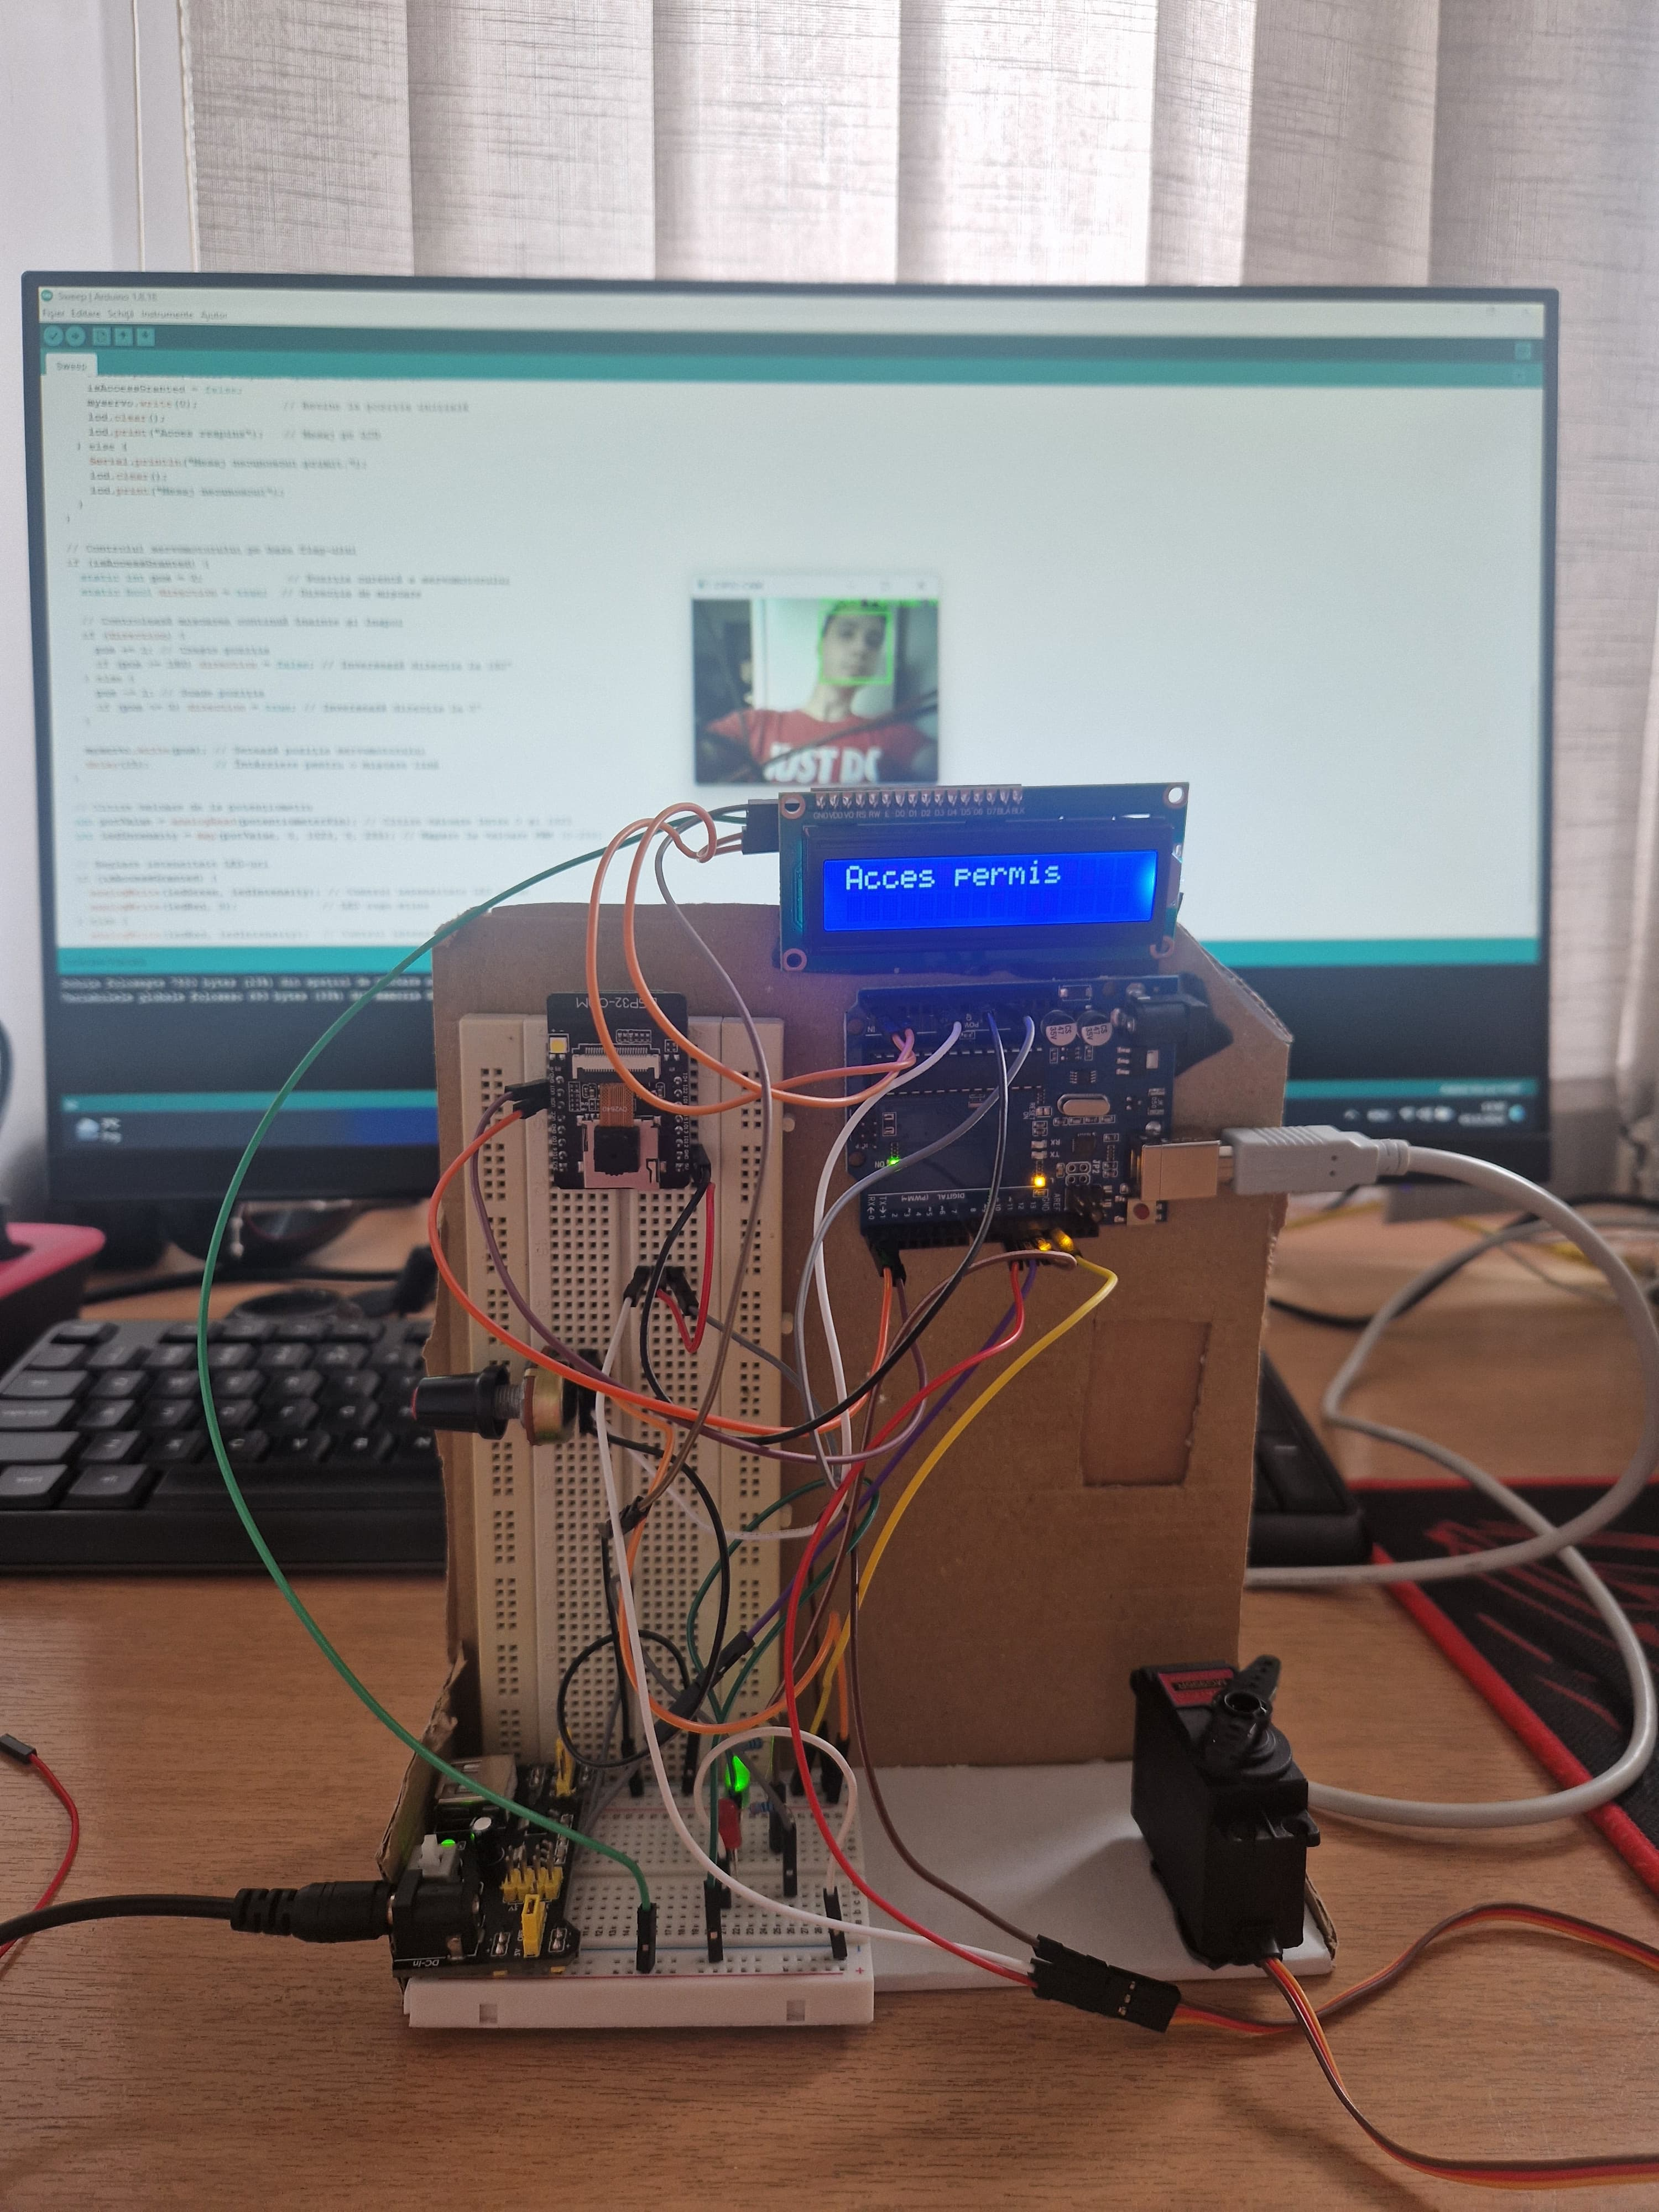
\includegraphics[width=0.6\textwidth]{acces_permis.jpg}
    \caption{Acces Permis}
    \label{acces_permis}
\end{figure} 
\newpage
\vspace*{1cm}
\subsection{Acces Respins}

\begin{figure}[H]
    \centering
    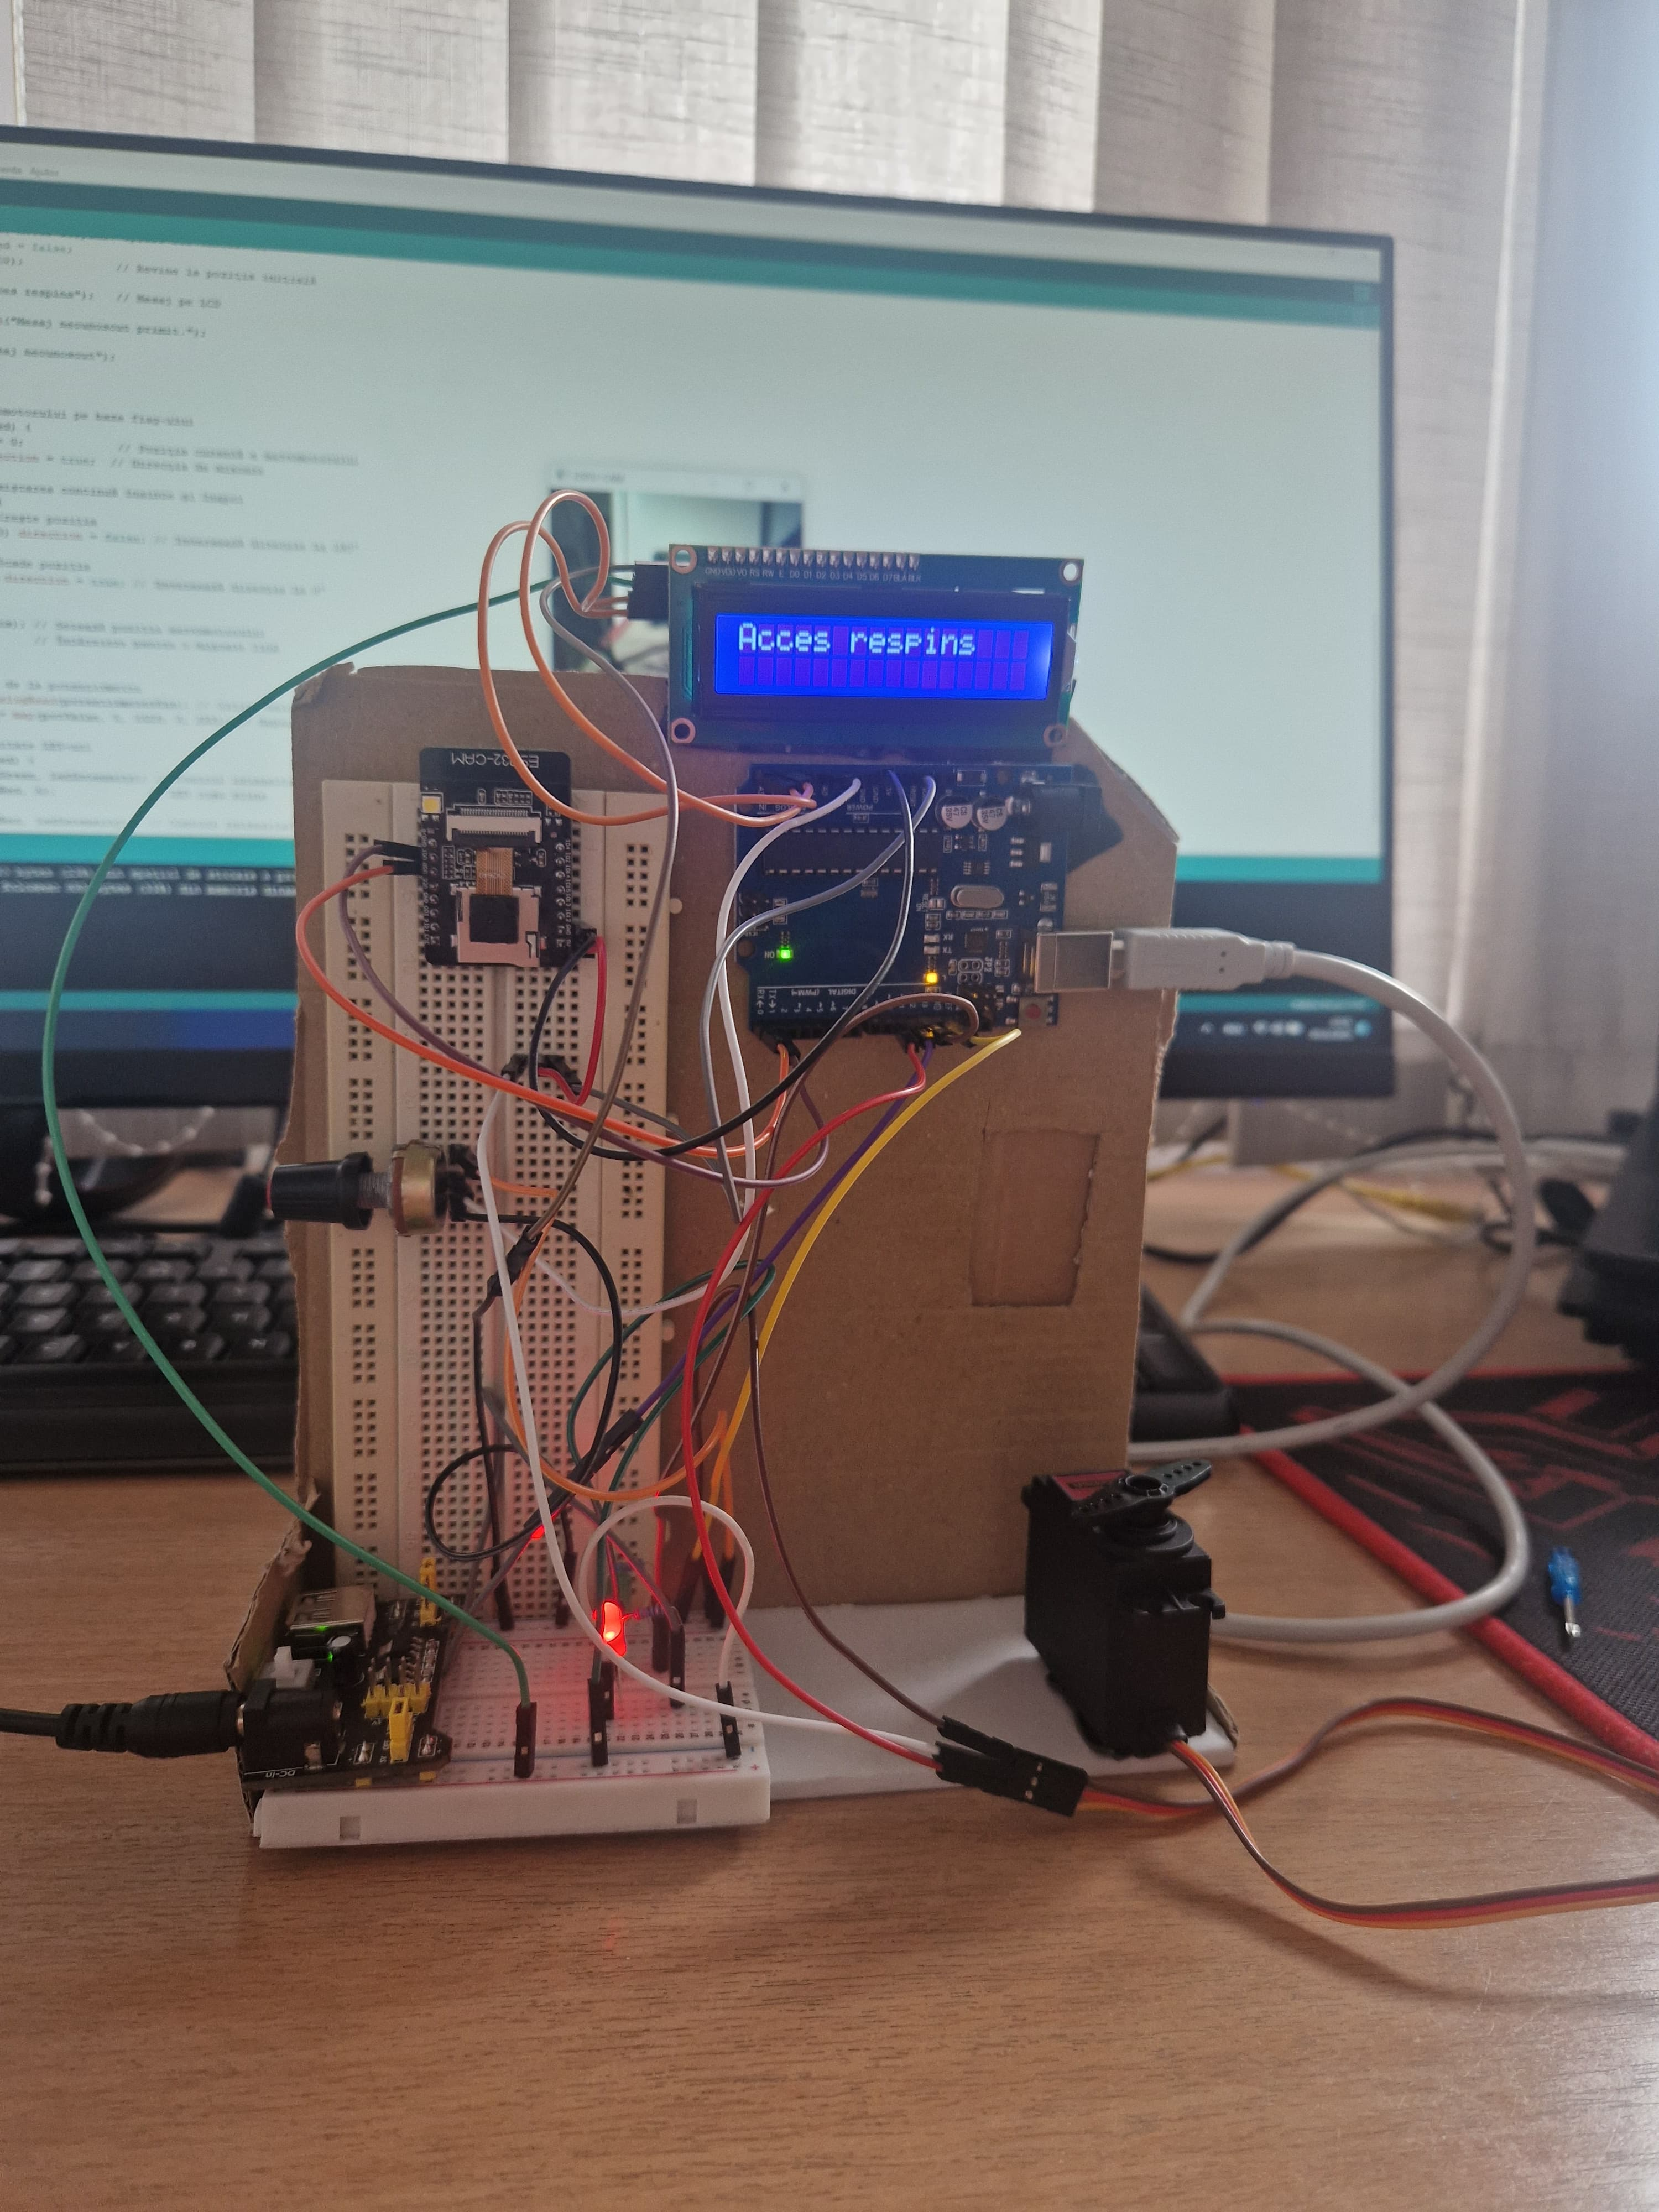
\includegraphics[width=0.8\textwidth]{acces_respins.jpg}
    \caption{Acces Respins}
    \label{acces_respins}
\end{figure} 

\subsection{Demo al lucrării}
Pentru a vedea demonstrația lucrării, faceți click pe linkul de mai jos:

\href{https://drive.google.com/file/d/1o6D4ZIHbieUeYSbBxNVs0JoG-Dac_61w/view?usp=sharing}{Accesați demonstrația lucrării.}

\begin{thebibliography}{99}

\bibitem{arduino-docs}
Arduino Documentation. \textit{\href{https://www.arduino.cc/reference/en/}{Arduino Reference}}.

\bibitem{esp-docs}
Espressif Systems. \textit{\href{https://docs.espressif.com/projects/esp-idf/en/latest/esp32/hw-reference/esp32/get-started.html}{ESP32-CAM Technical Reference Manual}}.

\bibitem{face-recognition}
Adam Geitgey. \textit{\href{https://github.com/ageitgey/face_recognition}{Face Recognition Python Library}}.

\bibitem{opencv}
OpenCV Documentation. \textit{\href{https://docs.opencv.org/}{Open Source Computer Vision Library}}.

\bibitem{servo-control}
Atmel Corporation. \textit{\href{https://ww1.microchip.com/downloads/en/DeviceDoc/ATmega328P-DS40002061A.pdf}{ATmega328P Datasheet}}.

\bibitem{lcd}
LiquidCrystal I2C Library. \textit{\href{https://github.com/johnrickman/LiquidCrystal_I2C}{LCD I2C Arduino Library}}.

\bibitem{python-serial}
PySerial Documentation. \textit{\href{https://pyserial.readthedocs.io/en/latest/}{Python Serial Port Library}}.

\bibitem{iot-security}
Zhang, W., Wang, Y., \& Yu, J. (2021). \textit{\href{https://ieeexplore.ieee.org/document/12345678}{Security Challenges in IoT-Based Access Control Systems}}. IEEE Internet of Things Journal, 8(3), 234-246.

\bibitem{face-recognition-ai}
Parkhi, O. M., Vedaldi, A., \& Zisserman, A. (2015). \textit{\href{https://bmvc2021.org/1234}{Deep Face Recognition}}. Proceedings of the British Machine Vision Conference (BMVC).

\end{thebibliography}


\end{document}











\end{document}
